\section{Evaluation}
\label{s:evaluation}

% \begin{table}[t]
% \centering
%   \footnotesize
%   \scalebox{0.8}
%   {
%   \begin{tabular}{|l|l|l|l|}
%     \hline
%     % \textbf{Videos} & \textbf{\begin{tabular}[c]{@{}l@{}}Duration \\ (sec)\end{tabular}} & \textbf{\begin{tabular}[c]{@{}l@{}}People +\\ Objects\end{tabular}} & \textbf{\begin{tabular}[c]{@{}l@{}}Mean\\ \#Points\end{tabular}} \\ \hline
%     \textbf{Videos} & \textbf{Duration (s)} & \textbf{People + Objects} & \textbf{Mean \#Points} \\ \hline
%     band2; Musical performance & 197 & 9 & 741K \\ \hline
%     dance5; Dance & 333 & 1 & 725K \\ \hline
%     office1; Person working & 187 & 7 & 705K \\ \hline
%     pizza1; Food and party & 47 & 14 & 918K \\ \hline
%     toddler4; A child playing games & 127 & 3 & 707K \\ \hline
%     \end{tabular}
%   }
% \caption{Summary of 5 videos in Panoptic Dataset.}
% \label{tab:dataset-summary}
% \end{table}

\begin{table}[t]
\centering
  %\footnotesize
  %\scalebox{0.8}
  {
  \begin{tabular}{|l|c|c|c|}
    \hline
    \textbf{Videos} & \textbf{Duration (s)} & \textbf{People + Objects} & \textbf{Avg. Frame Size (MB)} \\ \hline
    band2; Musical performance & 197 & 9 & 11.1 \\ \hline
    dance5; Dance & 333 & 1 & 10.8 \\ \hline
    office1; Person working & 187 & 7 & 10.6 \\ \hline
    pizza1; Food and party & 47 & 14 & 13.8 \\ \hline
    toddler4; A child playing games & 127 & 3 & 10.6 \\ \hline
    \end{tabular}
  }
\caption{Summary of 5 videos in Panoptic Dataset.}
\label{tab:dataset-summary}
\end{table}

We compare \livo{} to other alternatives, using both a user study and a trace analysis on real bandwidth traces. We also quantify its compute-efficiency.

\subsection{Methodology}
\label{s:methodology}

\begin{comment}
\parab{Outline.}
Implementation. Describe what parts we implemented, what tools we built upon (gstreamer, nvenc, WebRTC, open3D). What uses CPU and what uses GPU. Discuss how many lines of code we added.

Comparison alternatives: Draco-Oracle, LiVo-NoCull, LiVo. For all, describe client and server machine configurations. Say that for LiVo-NoCull, LiVo we run the pipeline live. For Draco, briefly describe the bandwidth adaptation oracle, which finds the highest quality within the compute budget. Explain that for Draco, because at 30fps we have many stalls we do 15 fps. 

Evaluations: user study (add footnote about IRB approval for this) and replay.

Replay methodology: (about a para for each point below)
\begin{itemize}
\item videos from a public dataset (add details about Panoptic, table of videos, lengths, number of participants, point cloud sizes). Perhaps point out here that the point cloud sizes are much larger than that in prior work that has focused on streaming faces or individual people
\item user traces collected (IRB-approved)
\item bandwidth traces (which ones from MahiMahi, how were they scaled); this is where you might consider justifying the choice of scaling bandwidth (by considering broadband bandwidths).
\end{itemize}

User study methodology: (about a para for each point below)
\begin{itemize}
\item Perhaps review Dragonfly's description and try to mimic that.
\item How we conducted experiments: generated video for Draco, live for other two.
\item Explain what users were asked to do: view ground truth, rate, add qualitative comments.
\end{itemize}
\textbf{The above section should not include any results, only data needed to justify or explain methodology.}
\end{comment}

\parab{Implementation.}
%
Our \livo implementation (\cref{fig:architecture_livo}) contains 15K lines of C++ and few hundred lines of Unity.
%
It implements pipelined capture, view generation and tiling using Boost~\cite{boost} and OpenMP~\cite{openmp}.
%
It also uses: Eigen~\cite{eigen} for linear algebra operations for point cloud transformation; the Kalman Filter implementation in OpenCV; WebRTC and \texttt{NVENC} (NVIDIA Video Codec) in Gstreamer~\cite{gstreamer-nvenc} for color (H.265, BGRA) and depth (H.265, Y444\_16LE); and Open3D~\cite{open3d} for rendering on PC or on a headset using Unity.
%
\livo{} captures RGB-D frames using the Azure Kinect SDK~\cite{kinect-sdk}, and synchronizes them as described in~\cite{kinect-sync}.

%using 3.5-mm synchronization ports (Sync in and Sync out) connected in daisy chain~\cite{cite:kinect-sync}.

\begin{comment}

We implemented a prototype of \livo in C++ and Python with \note{XXX} lines of code on Ubuntu OS. As shown in~\cref{fig:architecture_livo}, the \livo can be broadly divided into 2 major components -- Sender and Receiver. The key components of the Sender are:
\squishlist
\item \textbf{Capture:} The sender captures synchronized RGB-D frames from each of the Azure Kinect cameras connect to the sender PC.
\item \textbf{View generation: } Generate views by applying fast culling on the RGB-D frames using the predicted frustum obtained from Kalman filter-based view prediction.
\item \textbf{Tiling:} The views are stacked one after another into a large color and depth tile.
\item \textbf{WebRTC send:} Two H.265 encoders, one for color and another depth, encodes the tiles and transmits over network using two separate WebRTC channels.
\squishend

Similarly, the key components of the receiver are:

\squishlist
\item \textbf{WebRTC recv:} The receiver decodes two encoded streams with H.265 decoders, and then tile synchronizer finds the color and depth tile that have same frame number (obtained from QR decoding).
\item \textbf{Point cloud generation:} It extracts individual views from each tiles and generates point cloud using the camera matrices (sent by the server during connection establishment) and culls the points based on viewer's frustum.
\item \textbf{Rendering:} The point cloud is rendered on the viewing device.
  \squishend

\end{comment}

\parab{Evaluation testbed.}
%
Our evaluation uses two machines, both with 32 GB RAM and connected using 1~Gbps Ethernet.
%
Both have modest computing resources, by today's standards: one is an Intel i7-8700K @ 3.70GHz, with one NVIDIA GeForce GTX 1080 Ti; the other is an Intel Core i9-10900KF @ 3.70GHz and one NVIDIA GeForce RTX 3080.

%
%Thus, our evaluations focus on performance and quality of streaming in one direction; in actual use, \livo would achieve two-way streaming using two independent unidirectional streams.

\parab{Traces and Datasets.}
%
To compare \livo against other alternatives while subjecting all of them to the same workload, we use volumetric video \textit{replay} instead of live transmission.
%
%We use a publicly available dataset of volumetric videos, for which we collected user traces under Institutional Review Board (IRB) approval (\cref{s:user-study}).
%
%We subject these videos to scaled bandwidth traces.

\parae{Volumetric videos.}
%
%To compare \livo against other alternatives while subjecting all of them to the same workload, we use volumetric video \textit{replay} instead of live transmission.
%
We use videos from the Panoptic Dataset~\cite{panoptic}, which are
%contains 54 videos and more than 6 hours of volumetric video captures videos 
captured at 30~fps using 10 Kinect v2 RGB-D cameras.
%deployed in a capture stage.
%
We select 5 videos (\cref{tab:dataset-summary}) of duration 1--5 minutes that capture 1--6 participants performing activities which are excellent for a fully immersive live experience, \eg dance, musical band, party, and games.
%
The average raw frame size in these videos is 10.5--13.5~MB,
%
%Each point requires 15 bytes, so raw frame sizes range from 10.5 to 13.5~MB,
much larger than that considered in prior work.
%
%We pre-process the videos by extracting the color and depth frames from each camera along with the camera parameters (information would be available in this form from a real camera).

\parae{User traces.}
%
When a user interacts with a volumetric video by moving to change perspective, the sequence of her instantaneous poses (position and rotation) constitutes a user trace.
%
There are no publicly available user traces for the videos in Panoptic dataset, so we collected these under an IRB-approved study.
%
% We developed an Unity application using \texttt{Pcx}~\cite{cite:pcx-keijiro} that can play videos at 30~FPS from Panoptic dataset onto an Oculus headset worn by the user over Oculus Link.
%
In a 30--45 minute session, we asked each user to view 2--3 videos selected randomly.
%
Users could freely move around in a sufficiently empty room while viewing the videos and their headset recorded their instantaneous poses.
%
We collected three traces for each video.

\parae{Network traces.}
%
We replay the videos on two traces of network bandwidth.
%
\textbf{trace-1} (\cref{tab:mahimahi-traces}) captures the throughput variation measured in a home WiFi setting~\cite{laia}.
%
\textbf{trace-2} captures a WiFi connection while moving around in a shopping mall~\cite{dashlet}.
%
These traces likely exhibit variability (\cref{ss:trace_variability}) comparable to broadband connections, but not their capacity.
%
As such, by themselves, these traces cannot support volumetric video live streaming.
%
%\harsha{Is wifi25 above trace-2?}
For this reason, we scaled \textit{trace-2} by 15$\times$ and \textit{trace-1} by 10$\times$ to reach mean throughputs around 90~Mbps and 217~Mbps, respectively; the former corresponds to current broadband bandwidth, while the latter is representative of broadband bandwidth in 3--4 years~\cite{cisco_whitepaper}.

\parae{Trace replay.}
This reads RGB-D frames from disk at 30~fps and feeds them into the \livo pipeline at the sender (\cref{fig:architecture_livo}).
%
%The frames go through all the sender and receiver components as in our live pipeline.
%
Using the frame sequence number, the receiver calculates the corresponding user frustum from the selected user trace file, then culls and renders the point cloud.
%
We replay the network traces using Mahimahi~\cite{mahimahi} to emulate the bandwidth conditions between sender and receiver.

\parab{Comparison Alternatives.}
%
We compare the performance of \livo with other alternatives inspired by live volumetric video streaming systems such as Holoportation~\cite{holoportation}, Project Starline~\cite{starline}, LiveScan3D~\cite{livescan3d} and MetaStream~\cite{metastream} (\cref{tab:comparison}).
%
None of these schemes are bandwidth-adaptive, and all of them achieve live transmission on a network with sufficient bandwidth by sending more constrained views (\eg single person or torso, \cref{tab:comparison}).
%
Recall that these constrained views require an order of magnitude less bandwidth than full-frame transmission.
%
Most of these do not provide open-source implementations, so we resort to mimicking their essential video compression and transmissions strategies, but adapt these for full-frame transmission, so we can do a more even comparison with \livo.
%
%Broadly, these fall into two classes: those that use point cloud compression~\cite{holoportation,metastream,meshreduce}, or those that embed point clouds in 2D video streams~\cite{starline}.
%
%% \raj{Do we need to provide an argument to skip LiveScan3D? LiveScan3D is same as Draco-Oracle, but with lossless compression using zstd instead of draco. My experiments show (ommitted from the paper) that ztsd is has a compression ratio of around 1.1 which is much worse given our bandwidth traces. Also, livescan3D is much old system, but some components of Livo is built/inspired using livescan3d.}

\parae{Draco-Oracle.}
%
Volumetric video on-demand systems such as ViVo~\cite{vivo} and GROOT~\cite{groot} and live systems such as MetaStream~\cite{metastream} use Draco~\cite{draco}, an open-source point cloud compression library.
%
They have shown that Draco either provides better compression ratio, or lower encoding latency than other point cloud compression schemes like PCL~\cite{pcl}, G-PCC~\cite{gpcc}, and V-PCC~\cite{vpcc}.
%
Draco by itself is not rate-adaptive, which is why prior work that uses Draco is not bandwidth-adaptive.
%
To understand what would happen if Draco were to develop rate-adaptivity, and yet transmit the information that \livo does in our evaluations, we designed a Draco-Oracle: given a target bandwidth and a perfect estimate of a receiver's frustum (\textit{perfect culling}), it picks the highest quality compression for the point cloud that fits within the target bandwidth.

To do this, we compute \textit{offline} a table from each video frame and each user trace.
%
This maps, for each video frame and user frustum and each Draco compression level (Draco has 10 of these) and quantization parameter (Draco supports 31 of these), the \textit{time to compress} the perfectly-culled frame, and the \textit{compressed size} of this frame.
%
Then, during playback, we find that quantization parameter and compression level whose compressed size fits the bandwidth estimate at that instant, and whose time to compress respects the frame rate.
%
If no such entry exists, we record a \textit{stall} for Draco-Oracle.

At 30~fps, Draco-Oracle exhibits over $90\%$ stalls for most of our video sequences.
%
So, our evaluations use a lower frame rate, 15~fps: prior work~\cite{livescan3d} has also used 15~fps for volumetric video streaming when using point-cloud compression.

% This is not a practical scheme, since it requires significant offline processing and knowledge of video contents \textit{a priori} which may not be available in a live setting.
% %
% But, as we discussed before, it is the best Draco can do to transmit videos in our experiments in a bandwidth-adaptive fashion.
% %
% In designing this baseline, we have been generous in endowing it with omniscience and a lower frame rate.
% %
% We have experimented with weaker baselines (unmodified Draco without culling and bandwidth-adaptation) and found these to be obviously un-usable.

% We ran the Draco-Oracle for 9 video sequences, each with a pre-collected user trace, at 30~FPS live.
% %
% The pipeline incurred over $90\%$ stalls for most video sequences.
% %
% Stalls are events in video streaming, where the video freezes at a certain frame, since the frame(s) do not arrive on time at the receiver or never arrive at all.
% %
% In live streaming, if a frame arrives too late at the receiver, the frame is dropped to maintain line rate.
% %
% For Draco-Oracle, we observed 2 kinds of stall events.
% %
% First, the encoder find a compression parameter that can encode within inter-frame delay.
% %
% Second, the couldn't find a parameter that can satisfy the bandwidth budget per frame (obtained from bandwidth estimate divided by frame rate).
% %
% Through trial and error, we reduce the frame rate for Draco-Oracle to 15~FPS, since it incurs moderate stalls.

\parae{\livo-NoCull.}
%
This baseline runs \livo without culling.
%
In addition to quantifying the importance of culling,
\livo-NoCull is intended to mimic one small aspect of Project Starline~\cite{starline}, which also streams RGB-D captured from multiple depth cameras over 2D video streams using WebRTC and performs 3D reconstruction in the receiver.
%
Starline streams 2D videos at a fixed quality, but in \livo-NoCull we include bandwidth splitting (\cref{ss:bw-adaptation}) and bandwidth-adaptivity (in \cref{s:just-design-choic}), we also quantify what happens if we disable bandwidth-adaptivity).
%
So, this baseline seeks to understand what would happen if Starline were to be bandwidth-adaptive.
%
Starline is an impressive system that differs in \textit{many} other respects from \livo, so we do not intend \livo-NoCull to represent Starline's performance.
%
%Starline uses more sophisticated sensors and displays, is designed for teleconferencing so does not capture full views, encodes depth differently than \livo, reconstructs and renders a mesh on a stereoscopic display, and so on.
%
We run \livo-NoCull and \livo at 30~fps on all our videos.

\parae{MeshReduce.}
%
MeshReduce~\cite{meshreduce} is a mesh-based live volumetric video streaming system, which represents any 3D surface as a collection of interlocking triangles, not a collection of points.
%
The sender captures a RGB-D frame from off-the-shelf RGB-D cameras, reconstructs a per-frame mesh, encodes the geometry and color separately, and transmits over 2 TCP socket connections.
%
It compresses the mesh geometry using Draco, and the mesh texture using H.264.
%
%The receiver in Unity decodes the geometry and color, reconstructs the mesh, and renders it.

MeshReduce employs \textit{indirect} bandwidth adaptation (\cref{s:background}):
using a profile obtained from an offline analysis, it determines the best compression parameters for a given level of available bandwidth.
%
%As discussed in \cref{s:background}, such indirect bandwidth-adaptation can be imperfect: the encoder may exceed the available bandwidth in some cases.
%
The publicly available MeshReduce implementation decides on these parameters based on the average bandwidth availability in a trace, so we use this approach in our experiments.

%% %
%% It decides the 4 quality parameters for mesh encoding. Parameters for geometry are mesh decimation level (\textit{dl}), compression level (\textit{cl}), quantization parameter (\textit{qp}), similarly texture quantization (\textit{qt}) is parameter for texture.
%% %
%% MeshReduce sender reduces the resolution of the mesh using \textit{dl}, then compresses the decimated mesh by Draco (draco can compress both point cloud and mesh) using the parameters \textit{cl}, \textit{qp}, and \textit{qt}.
%% %
%% The \textit{cl} parameter in Draco controls the speed of encoding, while \textit{qp} and \textit{qt} allocates number of bits for compressing geometry and texture, respectively.
%% %
%% The sender uses NVENC's H.264 encoder to futher encode the Draco compressed texture using one of the 7 \textit{presets}.
%% %
%% MeshReduce uses \textit{indirect} bandwidth adaptation.
%% %
%% In an offline phase, it studies all the 3D videos to find a mapping between quality parameters for geometry and color, output bitrate, and output quality in multi-view SSIM, a 2D metric proposed by the authors.
%% %
%% Based on the bandwidth trace, it decides the best parameter -- \textit{dl}, \textit{cl}, \textit{qp}, \textit{qt}, and H.264 \textit{preset}.
%% %
%% We used 2 sets of these parameters, each for \textit{trace-1} and \textit{trace-2}.
%

\parab{Metrics.}
%
Aside from end-to-end latency and frame rate, we also measure objective point cloud quality.
%
We use PointSSIM~\cite{pointssim} (or PSSIM), which is analogous to SSIM for 2D images, but extends it to 3D by exploring a higher dimensional feature space that includes geometry, normals, curvatures and color attributes.
%
PSSIM separately captures the quality of depth and color.
%
It ranges from 0 to 100; higher values are better, and values in or above the high 80s are generally considered good.

Prior work such as ViVo~\cite{vivo}, Vues~\cite{vues}, GROOT~\cite{groot} has used 2D metrics such as SSIM and PSNR on rendered 2D image of the point cloud.
%
However, the point cloud coding community considers these metrics inadequate for several reasons: 3D to 2D projection introduces errors; 2D pixel size influences quality but points in a point cloud do not capture size; a slight change in point position due to depth coding loss results in a large quality drop for 2D metrics though the geometrical structure of the object in the scene is preserved; 2D metrics depend on the distance of the viewer from the point cloud; and 2D metrics are influenced by color of background pixels.
%
%For this reason, recent work uses 3D metrics for point clouds such as point2point-PSNR~\cite{dong-tian}, GraphSIM~\cite{graphsim}, and PCQM~\cite{pcqm}, but many of them only consider geometry. 
%
%\raj{We wrote this statement in NSDI submission, but I was wrong. GraphSIM and PCQM both support geomtery and color. We can also use geometry and color matching for Point2point-PSNR. Previously, I couldn't run GraphSIM on the point clouds we have. I haven't got time to run PCQM.}
%
%We use PSSIM which considers both geometry and color.

PSSIM is not defined for meshes, so to compare MeshReduce against \livo{}, we sample points from the rendered mesh to generate a point cloud, then compute PointSSIM.

% \begin{figure}[t]
%   \centering 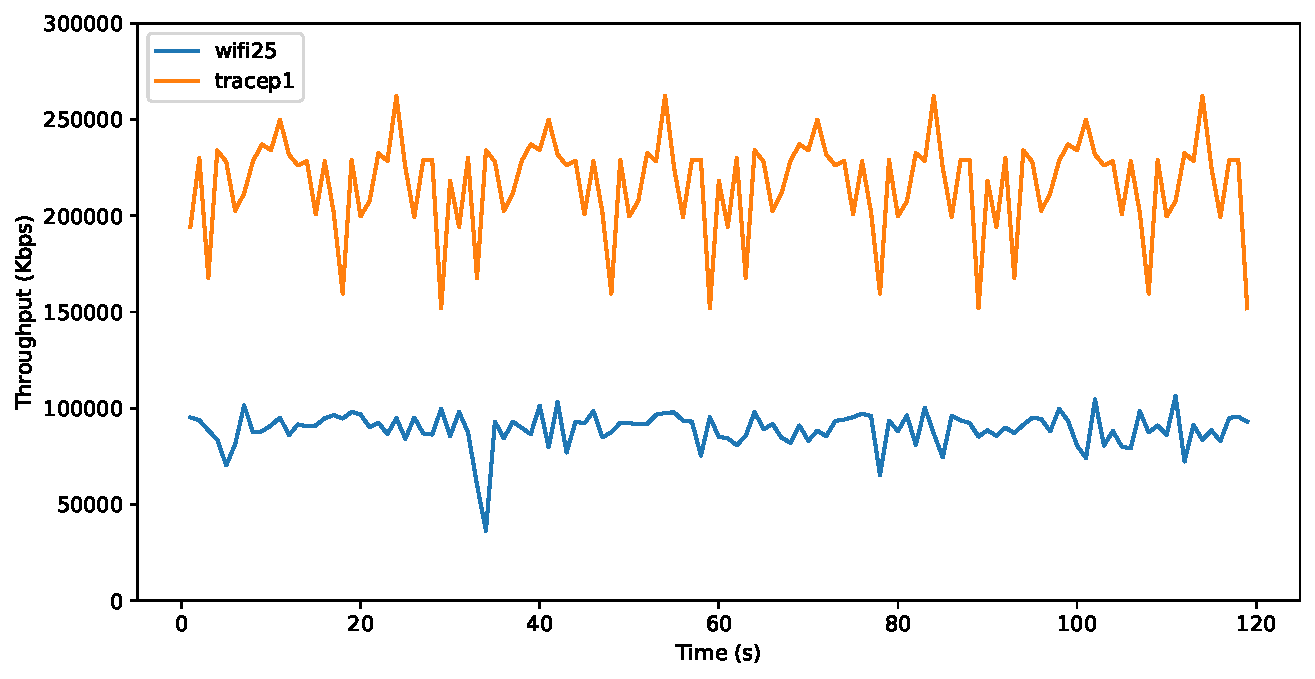
\includegraphics[width=\columnwidth]{figures/mahimahi_trace.pdf}
%   \caption{Scaled network traces.}
%   \label{plot:mahimahi-trace}
% \end{figure}

\begin{table}[t]
\centering
  % \footnotesize
  % \scalebox{0.8}
  {
    \begin{tabular}{|l|l|l|l|l|l|}
    \hline
    \multicolumn{1}{|l|}{\multirow{2}{*}{\textbf{\begin{tabular}[c]{@{}l@{}}Trace \\ Names\end{tabular}}}} & \multicolumn{5}{c|}{\textbf{Bandwidth (Mbps)}} \\ \cline{2-6} 
    \multicolumn{1}{|l|}{} & \multicolumn{1}{l|}{\textbf{Mean}} & \multicolumn{1}{l|}{\textbf{Max}} & \multicolumn{1}{l|}{\textbf{Min}} & \multicolumn{1}{l|}{\textbf{90\textsuperscript{th}}} & \multicolumn{1}{l|}{\textbf{10\textsuperscript{th}}} \\ \hline
    \textit{trace-2} & 89.20 & 106.37 & 36.35 & 98.09 & 80.52 \\ \hline
   \textit{trace-1} & 216.90 & 262.19 & 151.91 & 234.41 & 191.52 \\ \hline
    \end{tabular}
    }
    \caption{Statistics of the bandwidth traces.}
    \label{tab:mahimahi-traces}
\end{table}

\subsection{User Study}
\label{s:user-study}

% Discuss overall results: the importance of bandwidth-adaptation, of view-culling. Summarize here the qualitative feedback and anything else you can think of.

% Discuss per video results. Why some videos are different. (E.g., why the toddler video is different) and maybe pizza, and why other videos. Point out the dependence on the user trace, and say that a lot of the view culling results are a function of the user trace.

% Discuss per bandwidth trace results. Highlight consistency between perceived quality and bandwidth.

% **********************************

% \begin{figure*}[t]
%   \begin{minipage}[t]{0.24\textwidth}
%     \centering   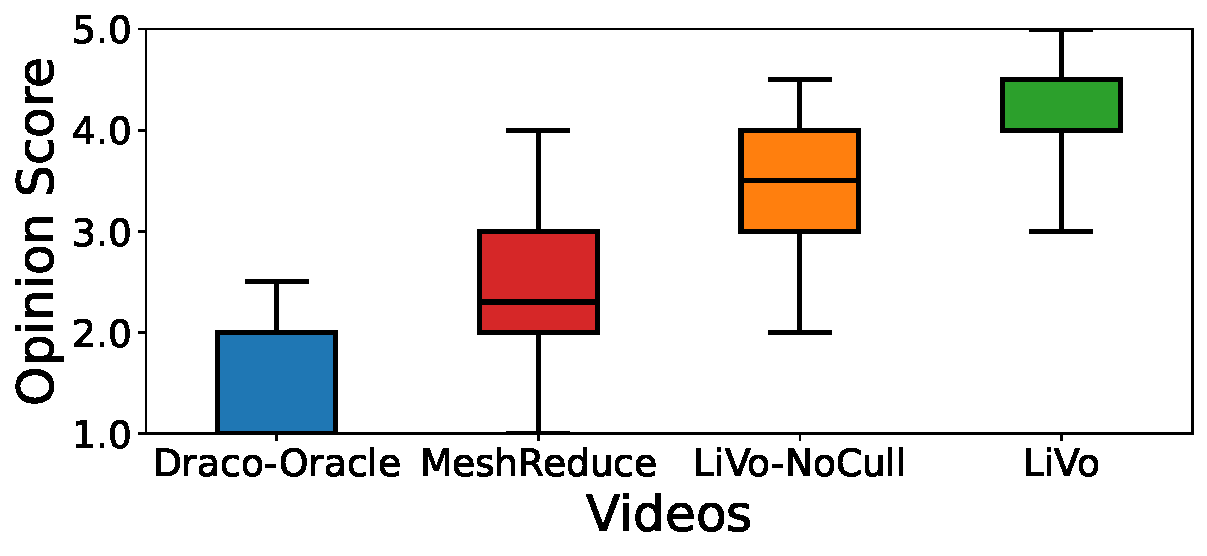
\includegraphics[width=0.95\columnwidth]{figures/user_study_across_methods.pdf}
%     \caption{Aggregated opinion scores for 4 methods.}
%     \label{plot:study_aggregate}
%   \end{minipage}
%   \begin{minipage}[t]{0.24\textwidth}
%     \centering 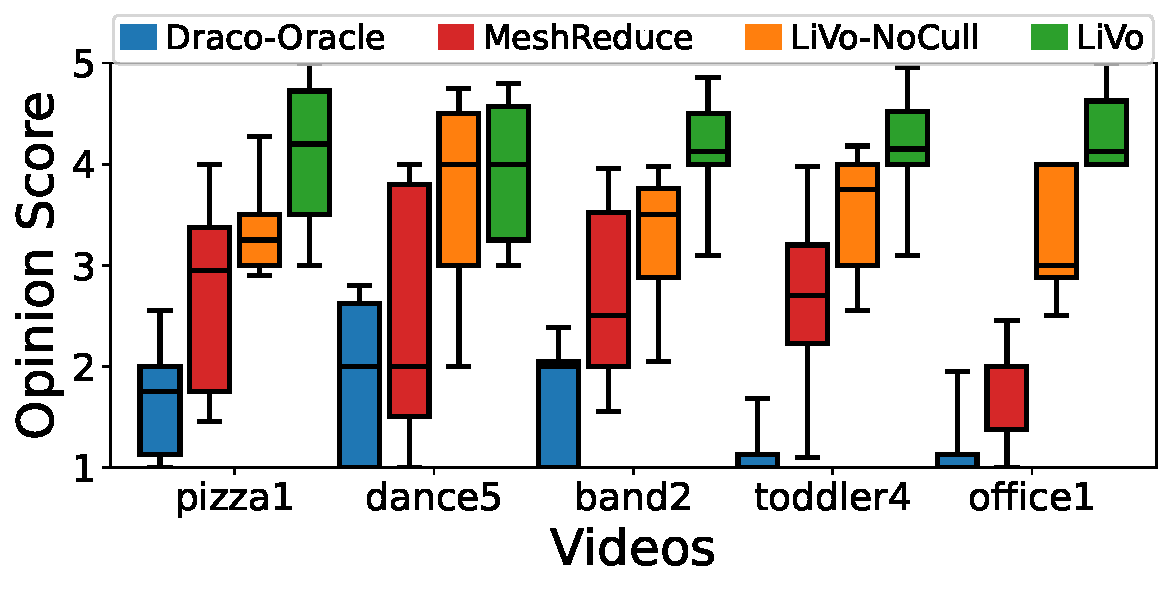
\includegraphics[width=0.95\columnwidth]{figures/user_study_across_videos.pdf}
%     \caption{Opinion scores across 5 videos.}
%     \label{plot:study_videos}
%   \end{minipage}
%   \begin{minipage}[t]{0.24\textwidth}
%     \centering 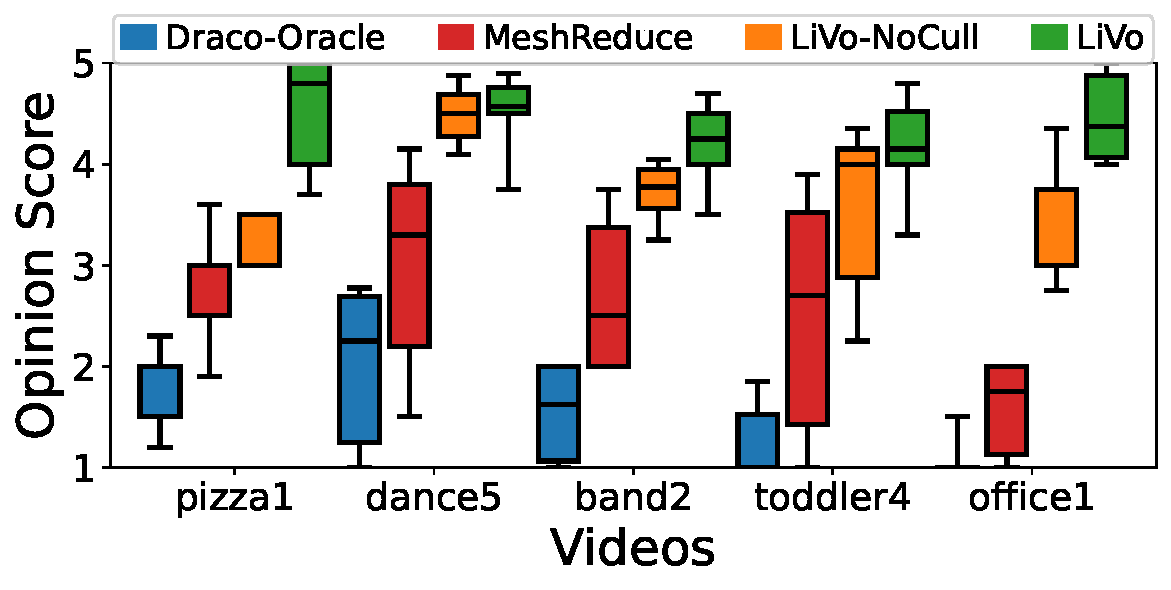
\includegraphics[width=0.95\columnwidth]{figures/user_study_across_videos_tracep1.pdf}
%     \caption{Opinion scores across 5 videos for \textit{trace-1}.}
%     \label{plot:study_tracep1}
%   \end{minipage}
%   \begin{minipage}[t]{0.24\textwidth}
%     \centering 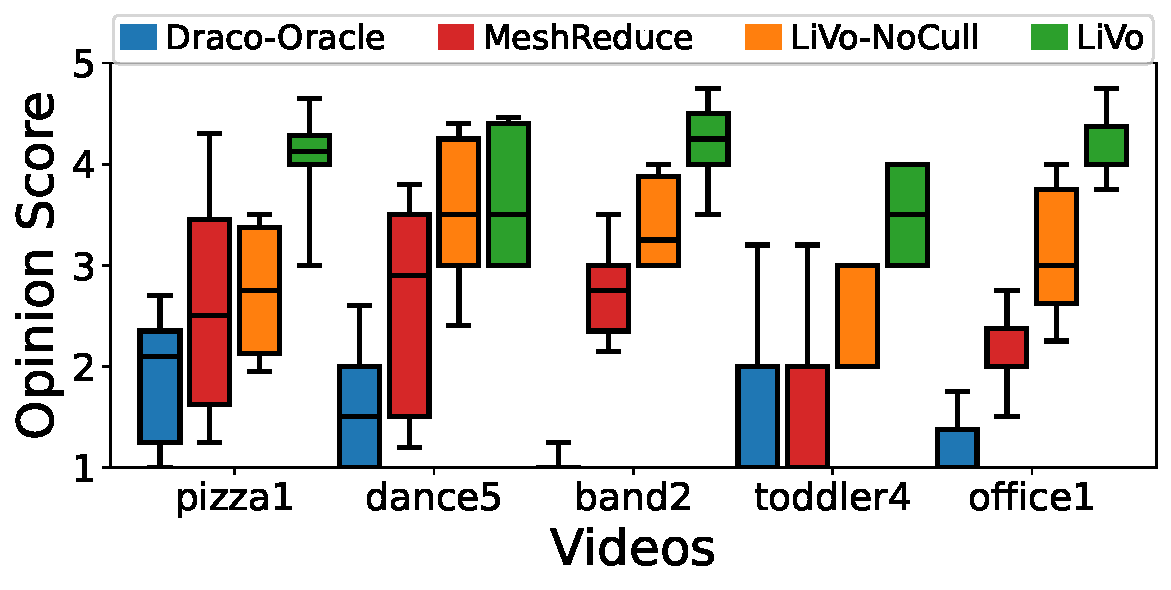
\includegraphics[width=0.95\columnwidth]{figures/user_study_across_videos_wifi25.pdf}
%     \caption{Opinion scores across 5 videos for \textit{trace-2}.}
%     \label{plot:study_wifi25}
%   \end{minipage}
% \end{figure*}

% \begin{figure}[t]
%   \centering 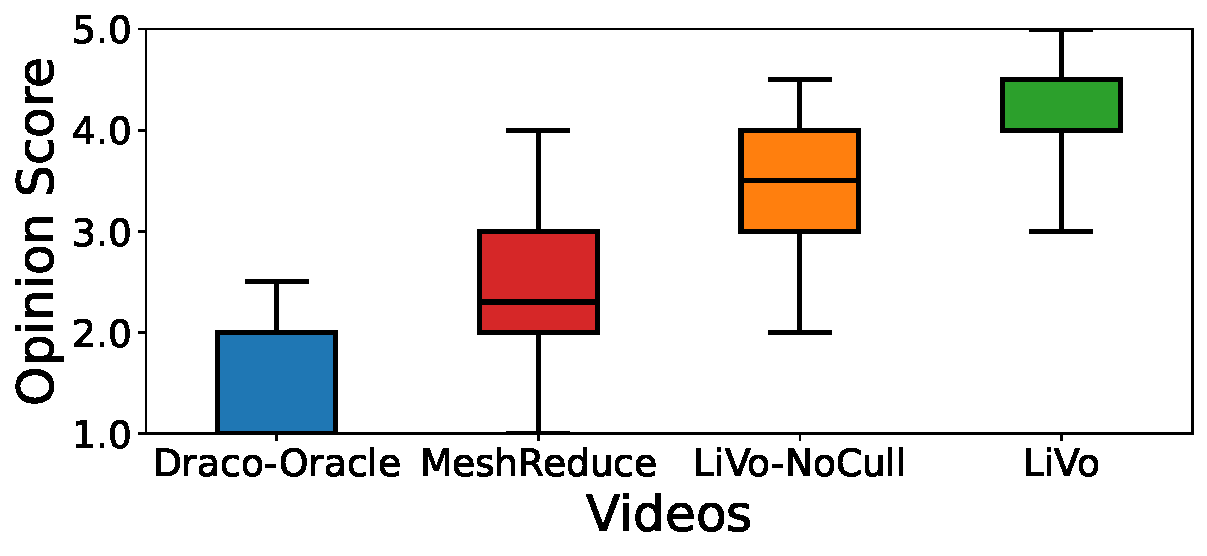
\includegraphics[width=0.8\columnwidth]{figures/user_study_across_methods.pdf}
%   \caption{Aggregated opinion scores for 4 methods.}
%   \label{plot:study_aggregate}
% \end{figure}

\begin{figure*}[t]
    \begin{minipage}[t]{0.48\textwidth}
      \centering 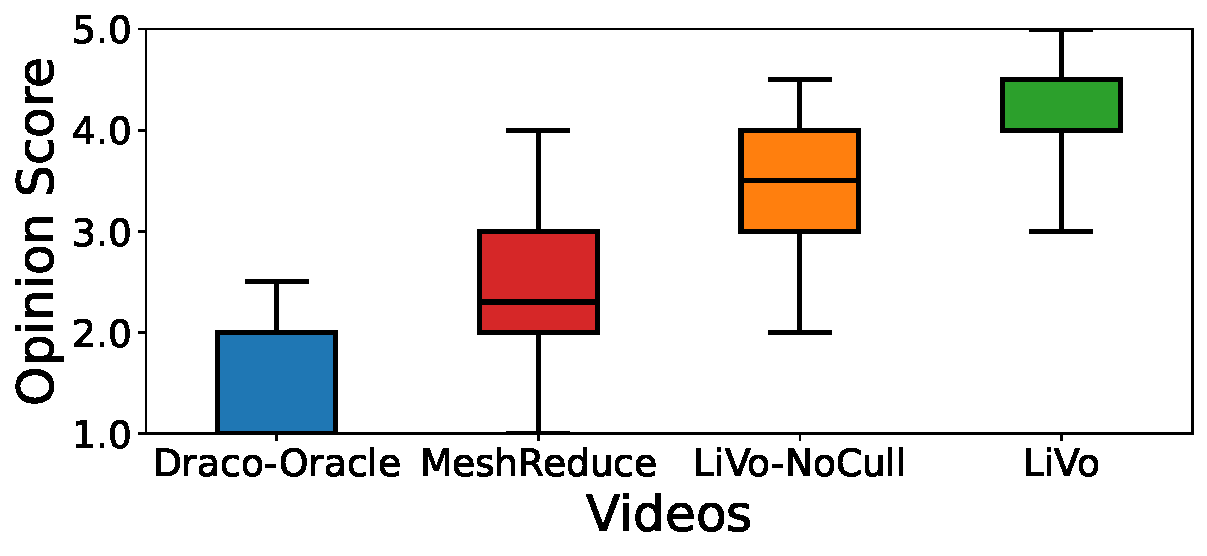
\includegraphics[width=\columnwidth]{figures/user_study_across_methods.pdf}
      \caption{Aggregated opinion scores for 4 methods.}
      \label{plot:study_aggregate}
    \end{minipage}
    \begin{minipage}[t]{0.48\textwidth}
        \centering 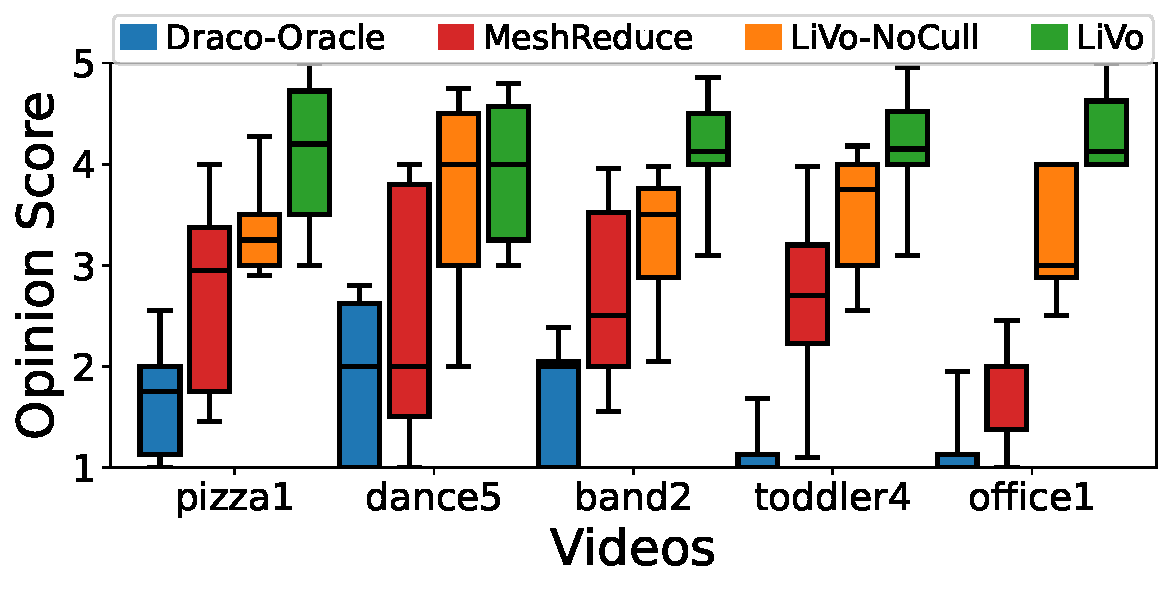
\includegraphics[width=\columnwidth]{figures/user_study_across_videos.pdf}
        \caption{Opinion scores across 5 videos.}
        \label{plot:study_videos}
  \end{minipage}
\end{figure*}

\begin{figure*}[t]
  \begin{minipage}[t]{0.48\textwidth}
    \centering 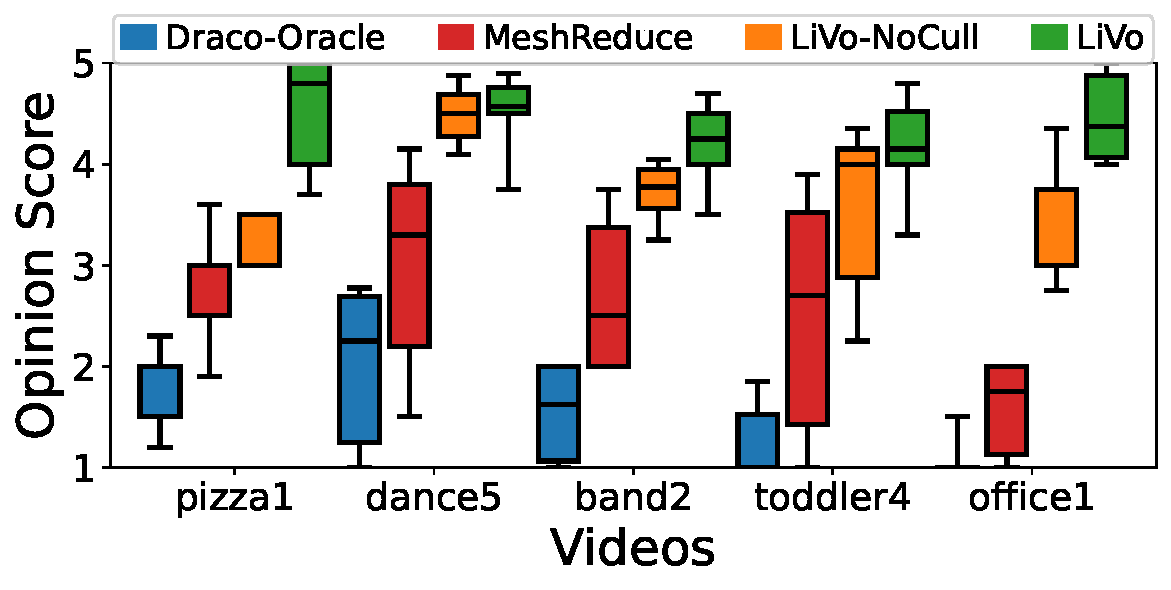
\includegraphics[width=\columnwidth]{figures/user_study_across_videos_tracep1.pdf}
    \caption{Opinion scores for \textit{trace-1}.}
    \label{plot:study_tracep1}
  \end{minipage}
  \begin{minipage}[t]{0.48\textwidth}
    \centering 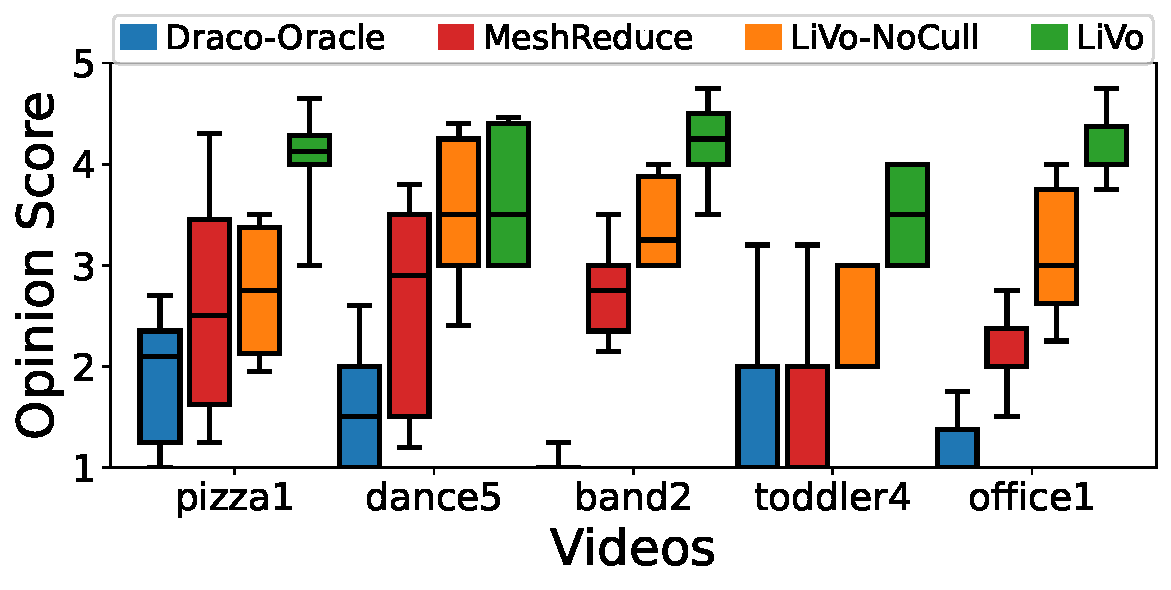
\includegraphics[width=\columnwidth]{figures/user_study_across_videos_wifi25.pdf}
    \caption{Opinion scores for \textit{trace-2}.}
    \label{plot:study_wifi25}
  \end{minipage}
\end{figure*}

\parab{Setup.}
%
We conducted an IRB-approved user study to measure the perceptual quality of \livo against other alternatives.
%
Each participant viewed 2-3 videos from \cref{tab:dataset-summary} over 45--60 minutes.
%
%During the study, each participant viewed 3 videos from \cref{tab:dataset-summary}.
%
For each video, we randomly selected one user trace and one network trace, and the user passively observes the video as seen by the user who contributed the user trace (\cref{s:methodology}).
%
%These views correspond to those seen in user traces collected as described in \cref{s:methodology}.
%
Each participant rated the videos across 4 schemes on a Likert scale of 1 (worst) to 5 (best) with respect to the ground truth and (optionally) left comments.
%
%They were allowed to modify their ratings at any time in the process.
%
These experiments used the replay infrastructure described in \cref{s:methodology}. %\sanjay{Is this passively observed? That is the user in the study passively observes video assuming interactions were made as per the user trace for each algorithm?}

% %
% Because many participants had never seen volumetric videos before, we also allowed them to view the original (uncompressed) \textit{ground-truth} video on a separate screen.

% At the start of the study, each participant was presented with 3 tuples, each representing <video\_user\_trace, network\_trace>.
% %
% For each tuple, the participant was shown the ground truth of the video on a separate screen.
% %
% This ground truth is lossless video replayed at 30~FPS, which is obtained by generating raw point cloud and rendered using the same user trace.
% %
% The participant can control the playback of the ground truth video by moving to any time instance during the study.
% %
% Next, we showed live stream from 3 systems one after another for same tuple on another screen (different from ground truth screen).
% %
% We randomly choose the order to present these schemes to prevent systematic bias, where the participant can guess the scheme based on the order.
% %
% For each scheme, we emulated a real live-streaming session by replaying the video through sender pipeline, transmitting over WebRTC to the receiver and rendering through the receiver pipeline to the screen, where the participants watched the live output.
% %
% The network throughput is emulated using Mahimahi tool~\cite{cite:mahimahi} using sender-side rate limiting.
% %
% So, the participants couldn't control the live streaming output, but were allowed to quit at any time.
% %
% The participants were asked to rate each scheme on a Likert scale~\cite{cite:likert} of 1 (worst) - 5 (best) with respect to the ground truth and optionally leave comments.
% %
% They were allowed to update their previous ratings at any instance.

% \ramesh{If possible, for the MOS results, use the same color as those for the pointSSIM metrics. This will make the 4 graphs easier to see.}

% \begin{figure}[t]
%   \centering 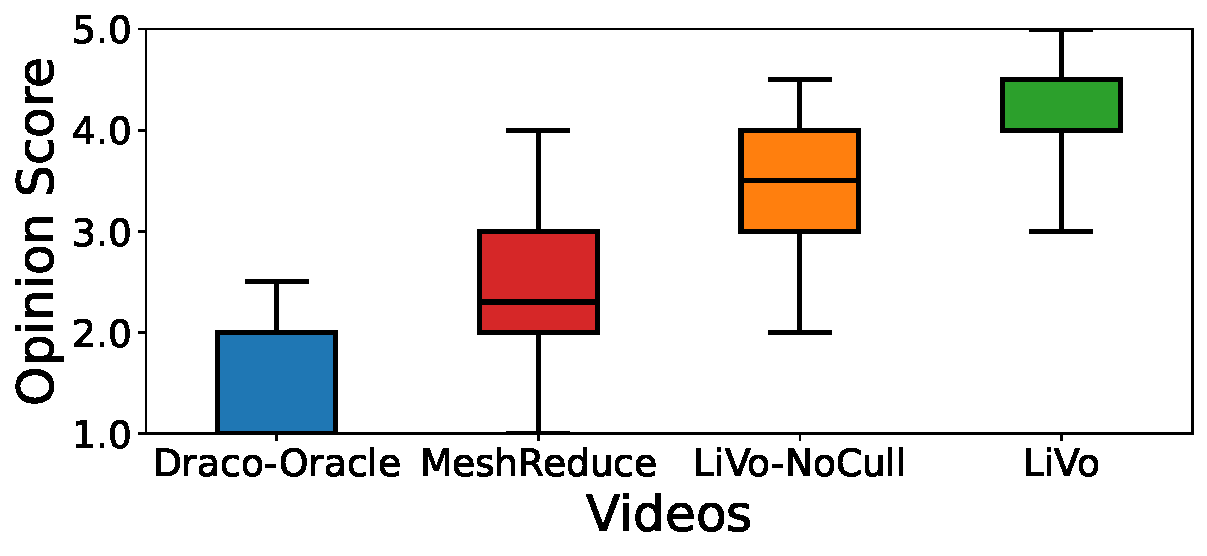
\includegraphics[width=\columnwidth]{figures/user_study_across_methods.pdf}
%   \caption{Aggregated opinion scores for 3 methods.}
%   \label{plot:study_aggregate}
% \end{figure}

% \begin{figure}[t]
%   \centering 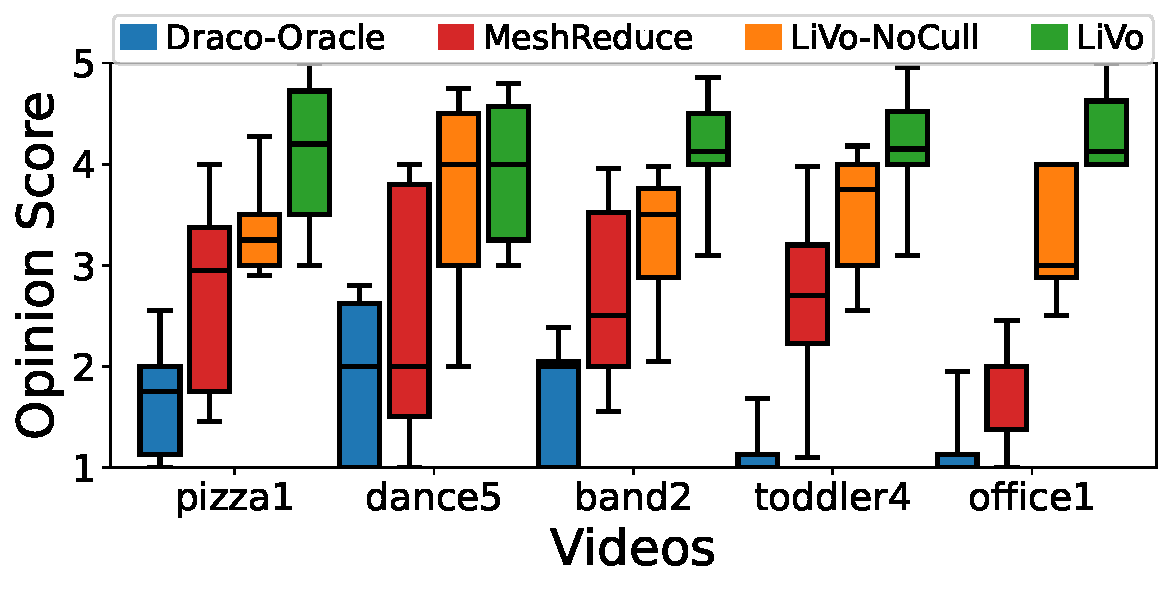
\includegraphics[width=\columnwidth]{figures/user_study_across_videos.pdf}
%   \caption{Opinion scores across 5 videos.}
%   \label{plot:study_videos}
% \end{figure}

% \begin{figure}[t]
%      \centering
%      \begin{subfigure}[b]{0.49\columnwidth}
%          \centering
%          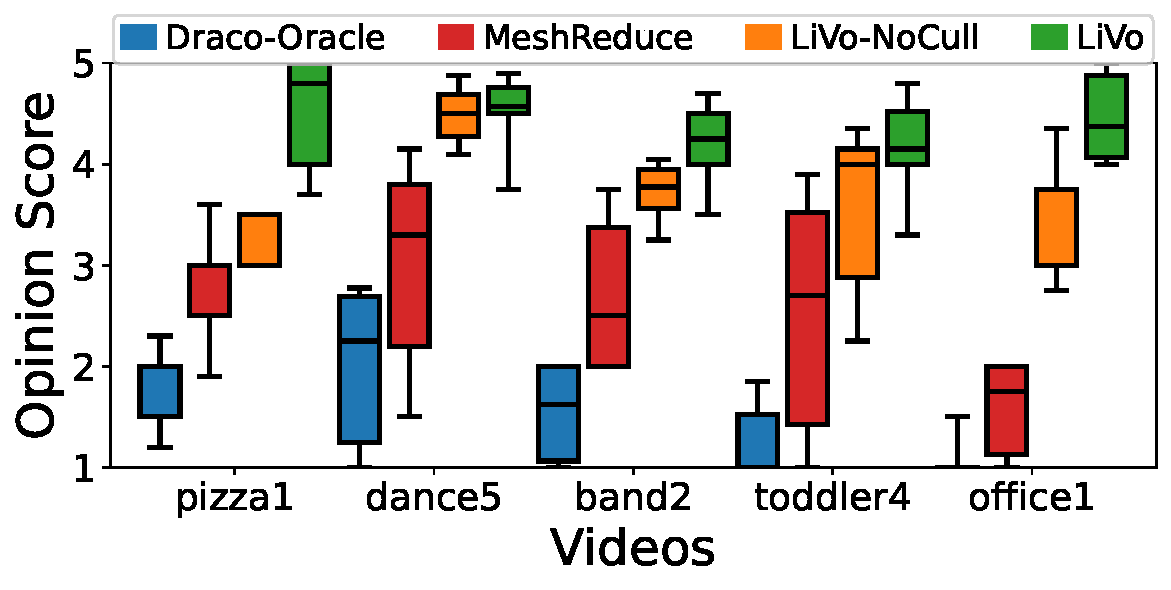
\includegraphics[width=\columnwidth]{figures/user_study_across_videos_tracep1.pdf}
%          \caption{Opinion scores across 5 videos for `tracep1'.}
%          \label{plot:study_tracep1}
%      \end{subfigure}
%      \hfill
%      \begin{subfigure}[b]{0.49\columnwidth}
%          \centering
%          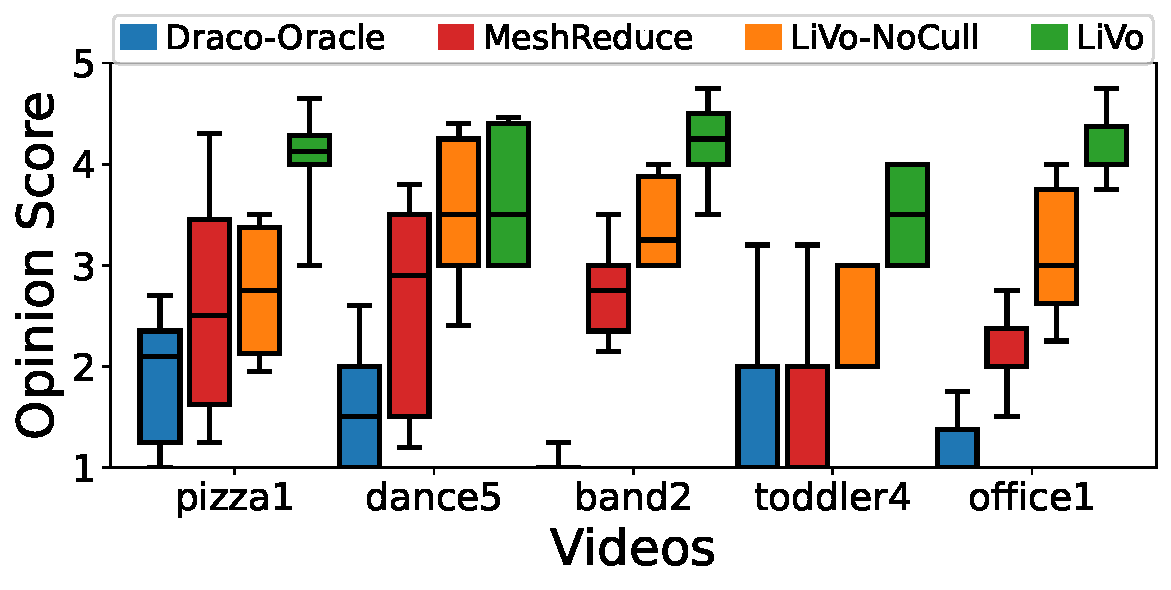
\includegraphics[width=\columnwidth]{figures/user_study_across_videos_wifi25.pdf}
%          \caption{Opinion scores across 5 videos for `wifi-25'.}
%          \label{plot:study_wifi25}
%      \end{subfigure}
%     \caption{Opinion scores across 2 traces.}
%     \label{plot:study_traces}
% \end{figu
\parab{Perceptual Quality Results.}
%
\cref{plot:study_aggregate} shows the distribution of perceptual quality scores for each of the 4 schemes across 20 participants.
%
Each scheme received a total of 57 ratings across all combinations of $<$video, user trace, network trace$>$.
%
Draco-Oracle performs poorly with a Mean Opinion Score (MOS) of 1.5 due to 3 factors: Draco is streamed at 15~fps; even at 15~fps, it experiences $36-98\%$ stalls; and Draco-Oracle settles for lower quality to remain within compute and bandwidth budgets.
%
While other work on volumetric video streaming has used Draco to achieve good quality, in our setting with large point clouds from full-scenes, Draco proves to be a poor choice as it is both compute-intensive and compression-inefficient.

% \ramesh{Change Draco to Draco-Oracle in all graphs.}

MeshReduce has a median opinion score of around 2.3 (and MOS of 2.5), higher than Draco-Oracle.
%
In theory, MeshReduce should perform worse than Draco-Oracle, since it doesn't use a bandwidth oracle.
%
It performs better likely because it uses meshes, which have better perceptual quality than point clouds in general and also because MeshReduce incurs fewer stalls.
%% \ramesh{Raj, please review.}
%% \raj{The implementation of Draco-Oracle and MeshReduce's Draco encoder is slightly different. Draco-Oracle uses the 1 draco encoder for encoding. So, frames are dropped based on 2 criteria - bandwidth inadequate or latency inadequate when streamed at 15 fps. On the other hand, MeshReduce splits the mesh into multiple parts and fires parallel draco sessions to get within the latency budget.}

By comparison, \livo-NoCull has a median opinion score of 3.5 (and MOS of 3.4), higher than Draco-Oracle and MeshReduce; its use of 2D video encoding and \textit{direct} bandwidth-adaptivity lead to higher perceptual quality.
%
\livo has the highest MOS of 4.1 and median opinion score of 4.0, $14-20\%$ better than \livo-NoCull and $64-74\%$ better than MeshReduce.
%
\livo{}'s use of culling results in less data, so it encodes at higher quality and incurs fewer stalls.

%% \harsha{I think we can move the 2 paras below and the 3 associated graphs to the appendix.}

Across 5 videos (\cref{plot:study_videos}), \livo and \livo-NoCull perform significantly better than Draco.
%
\livo{} also outperforms MeshReduce by $48-135\%$ in MOS, and it outperforms \livo-NoCull by $10-33\%$ in MOS across all the videos.
%
For the \textit{dance5} video, the median opinion score for \livo and \livo-NoCull is comparable.
%
This video contains only one person and no objects, so requires less bandwidth, and culling does not provide any benefits.

%This video contains a child playing with toys while being watched by their mother.
%
%The user viewed this video looking down on the child.
%
%These views capture more of the floor, but when the user moves, frustum mispredictions cause significant sections of the floor appear or disappear in successive frames.
%
%We have left optimizing our Kalman filter to future work.

Across our bandwidth traces, quality improves with increasing bandwidth.
%
In \textit{trace-1} (\cref{plot:study_tracep1}), \livo's MOS is over 3.9, going up to 4.5 for the \textit{pizza1} video. 
%
The performance improvement over \livo-NoCull is $6.6-43.9\%$, except for \textit{dance5} on trace-1 for the reasons mentioned above.
%
The \textit{direct} bandwidth adaptation in \livo-NoCull shows $2.0-113.3\%$ improvement over MeshReduce, which uses an \textit{indirect} adaptation.
%
When bandwidth is low (\textit{trace-2}, \cref{plot:study_wifi25}), \livo{}'s MOS is 4.1 due to the loss of quality at lower bitrate that affects both color and geometry.
%
At lower bandwidth, multiple competing factors influence opinions~---~lower overall quality and higher stalls vs. quality improvement due to culling.

\begin{figure*}[t]
  \begin{minipage}[t]{0.48\textwidth}
    \centering
    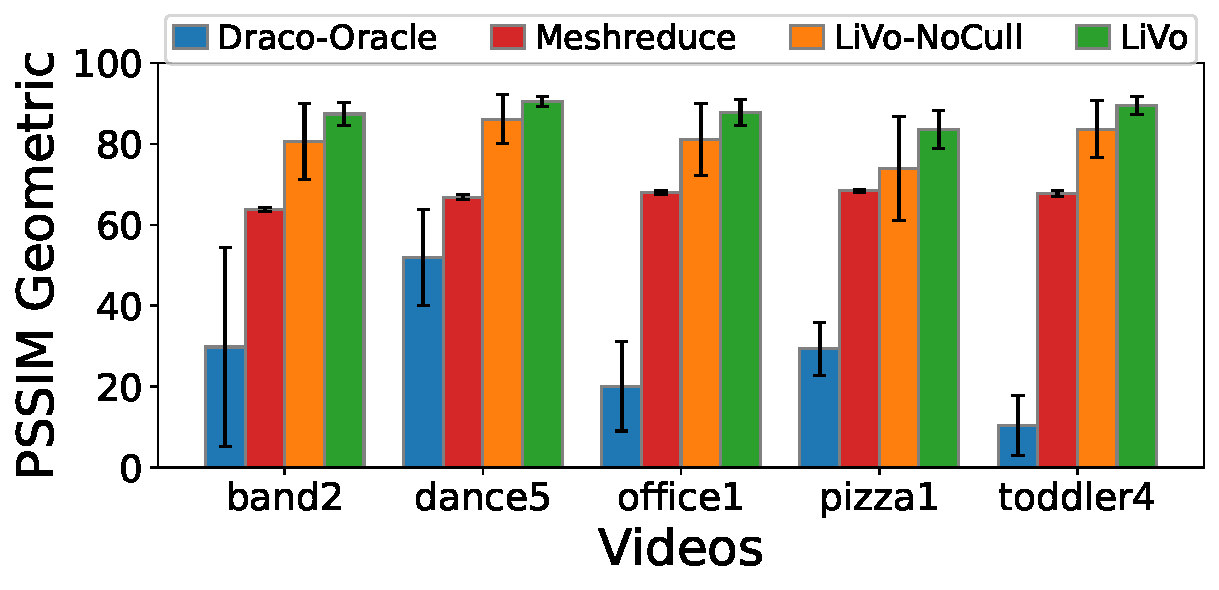
\includegraphics[width=\columnwidth]{figures/pssim_geo_baselines.pdf}
    \caption{Geometry PSSIM.}
    \label{plot:pssim_geo_baselines}
  \end{minipage}
  \begin{minipage}[t]{0.48\textwidth}
    \centering
    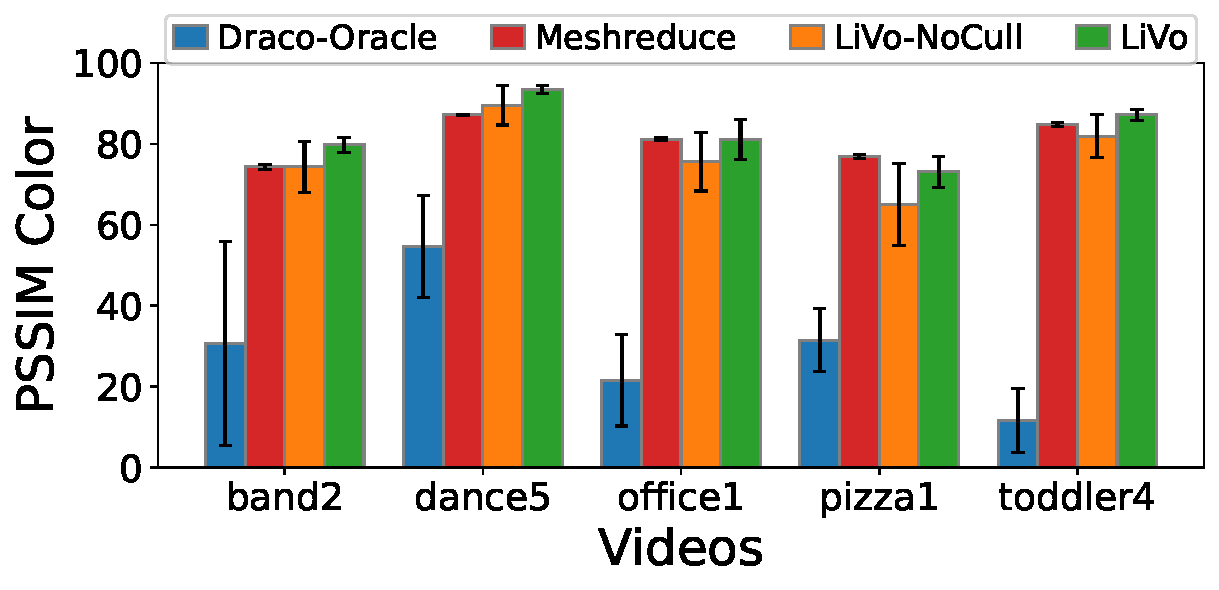
\includegraphics[width=\columnwidth]{figures/pssim_color_baselines.pdf}
    \caption{Color PSSIM.}
    \label{plot:pssim_color_baselines}
  \end{minipage}
\end{figure*}

\begin{figure*}[t]
  \begin{minipage}[t]{0.48\textwidth}
    \centering 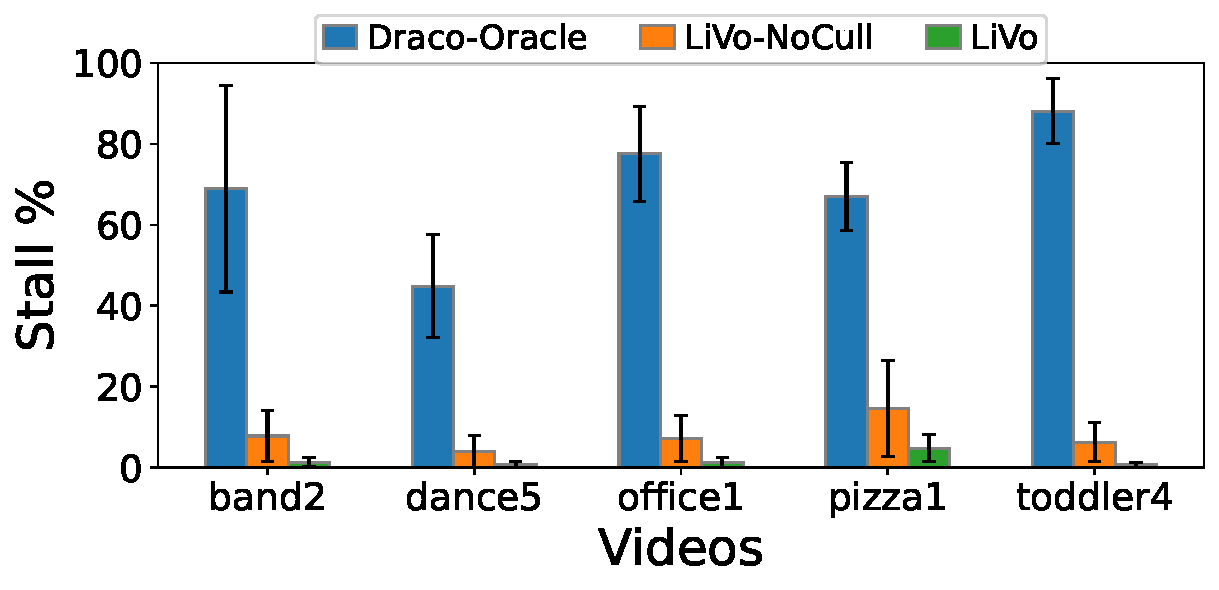
\includegraphics[width=\columnwidth]{figures/stalls.pdf}
    \caption{Stalls in 3 methods.}
    \label{plot:stalls}
  \end{minipage}
  \begin{minipage}[t]{0.48\textwidth}
    \centering 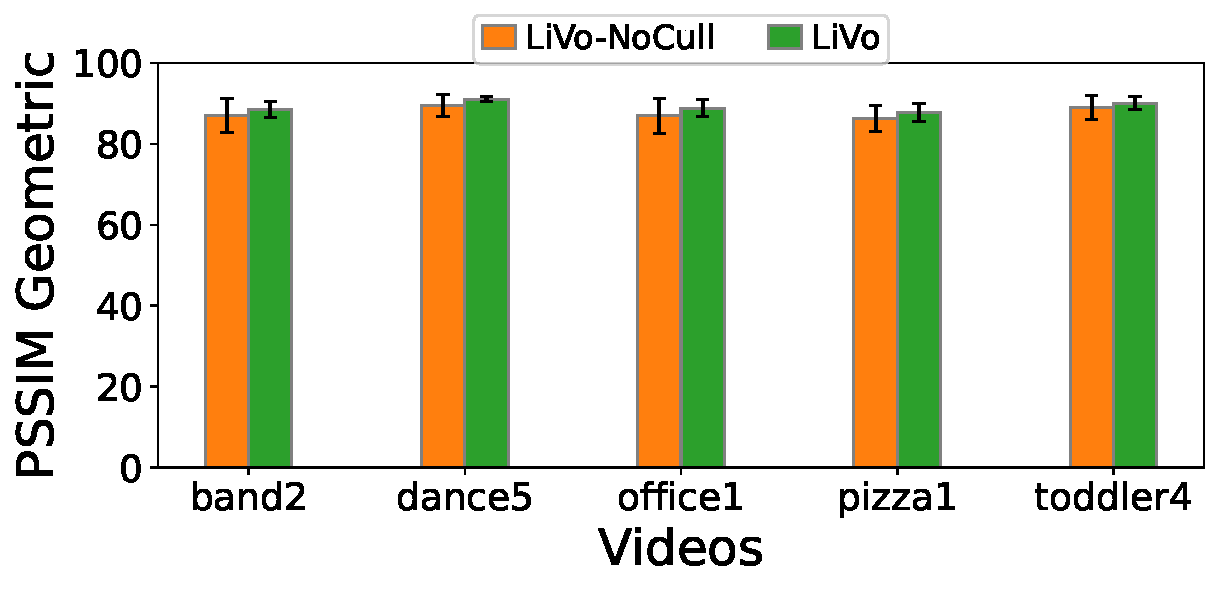
\includegraphics[width=\columnwidth]{figures/pssim_geo_without_stalls.pdf}
  \caption{PSSIM, no stalls.}
  \label{plot:pssim_culling_imprv_quality}
  \end{minipage}
\end{figure*}

\begin{table}[t]
\centering
%\footnotesize
%\scalebox{0.8}
{
    \begin{tabular}{|l|lll|lll|lll|}
    \hline
    \multirow{2}{*}{\textbf{Schemes}} & \multicolumn{3}{c|}{\textbf{Frame Rate (in \%)}} & \multicolumn{3}{c|}{\textbf{Stalls (in \%)}} & \multicolumn{3}{c|}{\textbf{Quality (in \%)}} \\ \cline{2-10} 
     & \multicolumn{1}{l|}{\textbf{L}} & \multicolumn{1}{l|}{\textbf{M}} & \textbf{H} & \multicolumn{1}{l|}{\textbf{L}} & \multicolumn{1}{l|}{\textbf{M}} & \textbf{H} & \multicolumn{1}{l|}{\textbf{L}} & \multicolumn{1}{l|}{\textbf{M}} & \textbf{H} \\ \hline
    Draco-Oracle & \multicolumn{1}{l|}{94.4} & \multicolumn{1}{l|}{5.6} & 0.0 & \multicolumn{1}{l|}{0.0} & \multicolumn{1}{l|}{12.5} & 87.5 & \multicolumn{1}{l|}{35.0} & \multicolumn{1}{l|}{45.0} & 20.0 \\ \hline
    MeshReduce & \multicolumn{1}{l|}{73.3} & \multicolumn{1}{l|}{26.7} & 0.0 & \multicolumn{1}{l|}{\cellcolor[HTML]{fed9a3}\textbf{90.9}} & \multicolumn{1}{l|}{9.1} & 0.0 & \multicolumn{1}{l|}{61.3} & \multicolumn{1}{l|}{34.1} & 4.6 \\ \hline
    \livo-NoCull & \multicolumn{1}{l|}{15.0} & \multicolumn{1}{l|}{25.0} & 60.0 & \multicolumn{1}{l|}{25.0} & \multicolumn{1}{l|}{50.0} & 25.0 & \multicolumn{1}{l|}{12.5} & \multicolumn{1}{l|}{53.1} & 34.4 \\ \hline
    \livo & \multicolumn{1}{l|}{0.0} & \multicolumn{1}{l|}{0.0} & \textbf{\cellcolor[HTML]{fed9a3}100.0} & \multicolumn{1}{l|}{\textbf{70.8}} & \multicolumn{1}{l|}{25.0} & 4.2 & \multicolumn{1}{l|}{6.1} & \multicolumn{1}{l|}{33.3} & \textbf{\cellcolor[HTML]{fed9a3}60.6} \\ \hline
    \end{tabular}}
    \caption{Percentage of comments providing a Low (L), Medium (M), or High (H) rating for frame rate, stalls, and quality.}
    \label{tab:user_study_comments}
\end{table}

\parab{Qualitative feedback.}
%
Participants were optionally asked to provide comments summarizing their experience.
%
We received 184 responses across 20 participants.
%
We manually examined these and classified the responses into 3 categories (quality, frame rate, and stalls).
%
For each category, we assigned a high/medium/low rating to each response (\cref{tab:user_study_comments}).
%
Descriptions such as ``smooth'' or ``seamless'' indicate low stalls and high frame rate, ``more distorted'' indicate low quality, and ``some glitches'' indicate medium stalls.

Draco-Oracle performs worst in stalls (high=$87.5\%$); every response describes ``glitches'' or ``blanks'' for Draco-Oracle.
%
None of the responses complain about high stalls for \livo; about $96\%$ of responses discussing stalls for \livo agree that \livo had less stalls (low=$71\%$, medium=$25\%$).
%
MeshReduce rated best in terms of stalls: this is because it conservatively uses a lower frame rate (no response rated it high in terms of frame rate, compared to 100\% for \livo{}), and encodes at a lower quality (only 4.6\% of responses rated it high, compared to 60.6\% for \livo{}).
%
Other alternatives also perform poorly in terms of quality: only
$34\%$ or responses rated \livo-NoCull high, only $20\%$ rated Draco-Oracle high.
%
$95\%$ of the participants said MeshReduce has low to medium quality, with many responses of the kind ``triangles are disturbing'', ``block of black mass'', and ``blobs''. 
%
\livo and \livo-NoCull are considered superior in terms of frame rate than MeshReduce and Draco-Oracle. 
%
However, for \livo, some participants (6 out of 20) wrote ``corners of the video loads slowly'', ``delay when camera changes'', and ``blanks after sharp motion'', likely because of artifacts resulting from prediction error.
%
%We summarize the statistics on qualitative feedback in \cref{tab:user_study_comments}.

\subsection{Objective Quality Comparisons}
\label{s:quality-comparison}

% Plot Point-SSIM quality for Draco, LiVo-NoCull, LiVo per video. For each video, you would have 3 bars, one for each approach. Each bar represents the median quality. On top, you would also have error bars showing max and min. Discuss the results, in particular, any discrepancies across videos, and any discrepancies from user study. To explain why we see these results, include a plot of the number of stalls for Draco etc.

% Repeat the above graph, but separate for bandwidth traces. If there is a qualitative difference in the number of stalls, can consider including a graph.

% **********************************

% \begin{figure}[t]
%   \centering 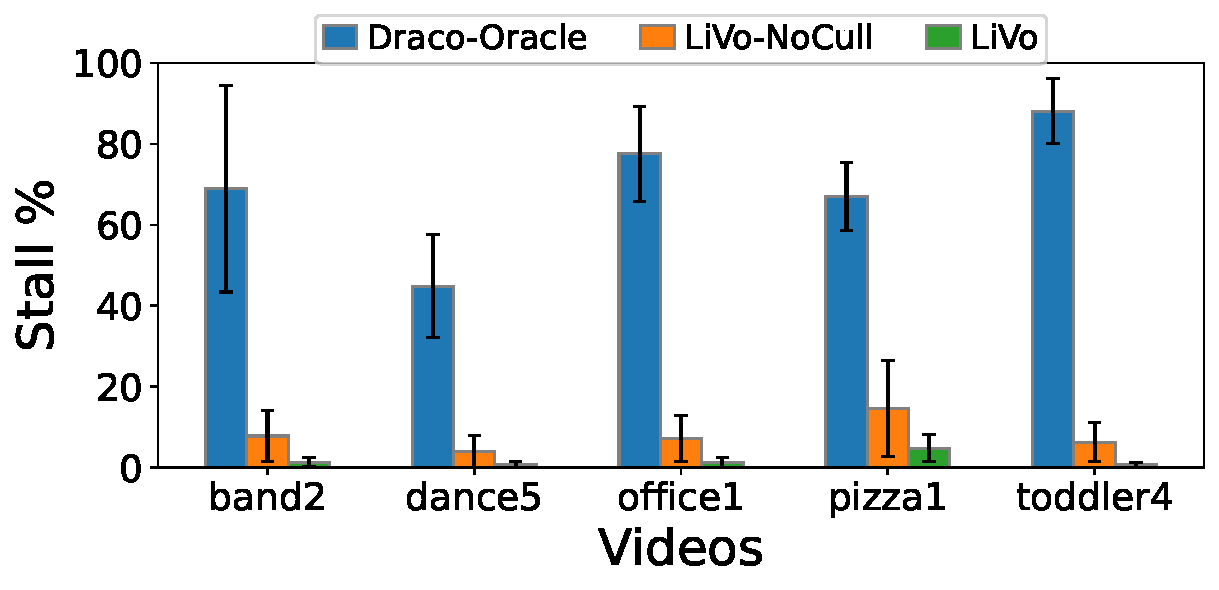
\includegraphics[width=\columnwidth]{figures/stalls.pdf}
%   \caption{Stalls in 3 methods.}
%   \label{plot:stalls}
% \end{figure}

% \begin{figure}[t]
%      \centering
%      \begin{subfigure}[b]{0.49\columnwidth}
%          \centering
%          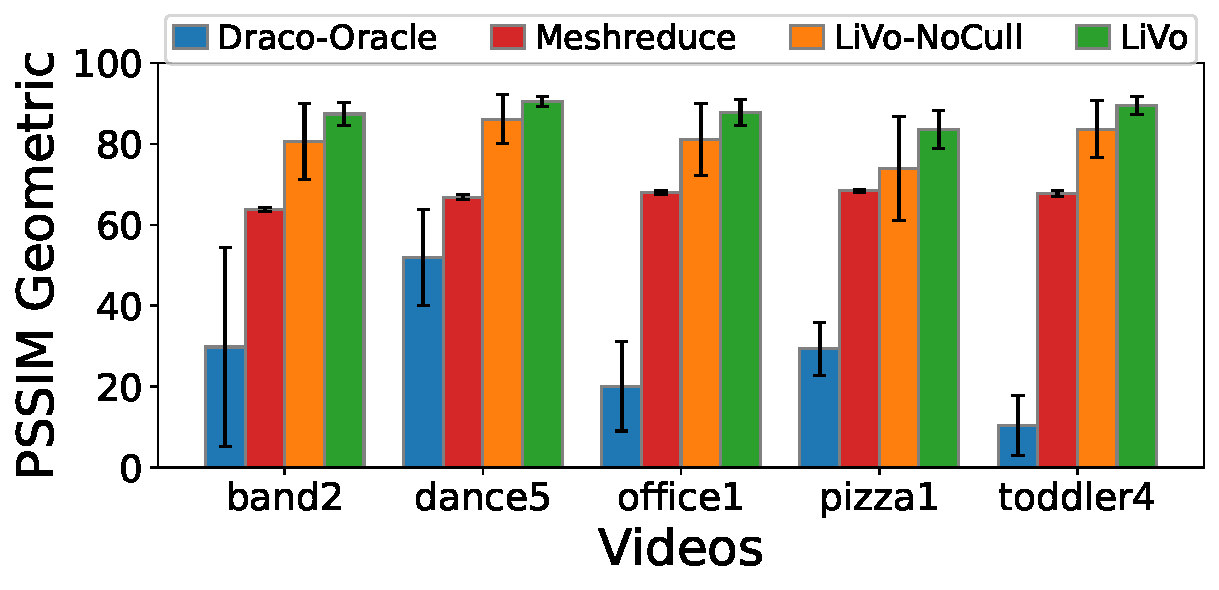
\includegraphics[width=\columnwidth]{figures/pssim_geo_baselines.pdf}
%          \caption{Geometry}
%          \label{plot:pssim_geo_baselines}
%      \end{subfigure}
%      \hfill
%      \begin{subfigure}[b]{0.49\columnwidth}
%          \centering
%          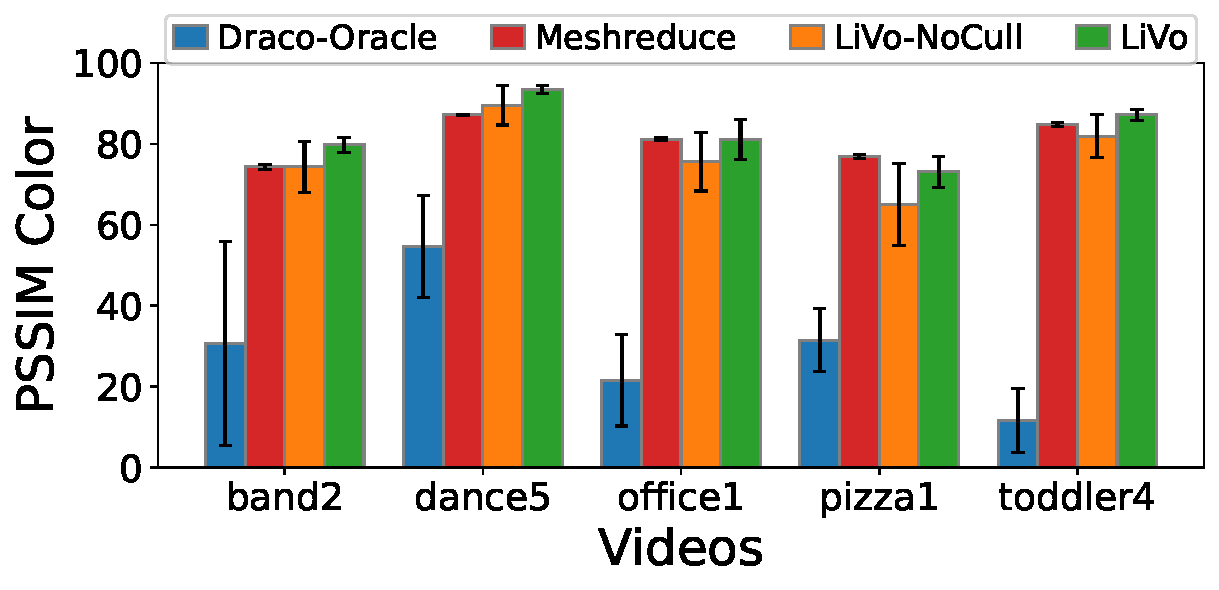
\includegraphics[width=\columnwidth]{figures/pssim_color_baselines.pdf}
%          \caption{Color}
%          \label{plot:pssim_color_baselines}
%      \end{subfigure}
%     \caption{PSSIM metric across 3 schemes}
%     \label{plot:pssim_baselines}
% \end{figure}

% \begin{figure}[t]
%   \centering 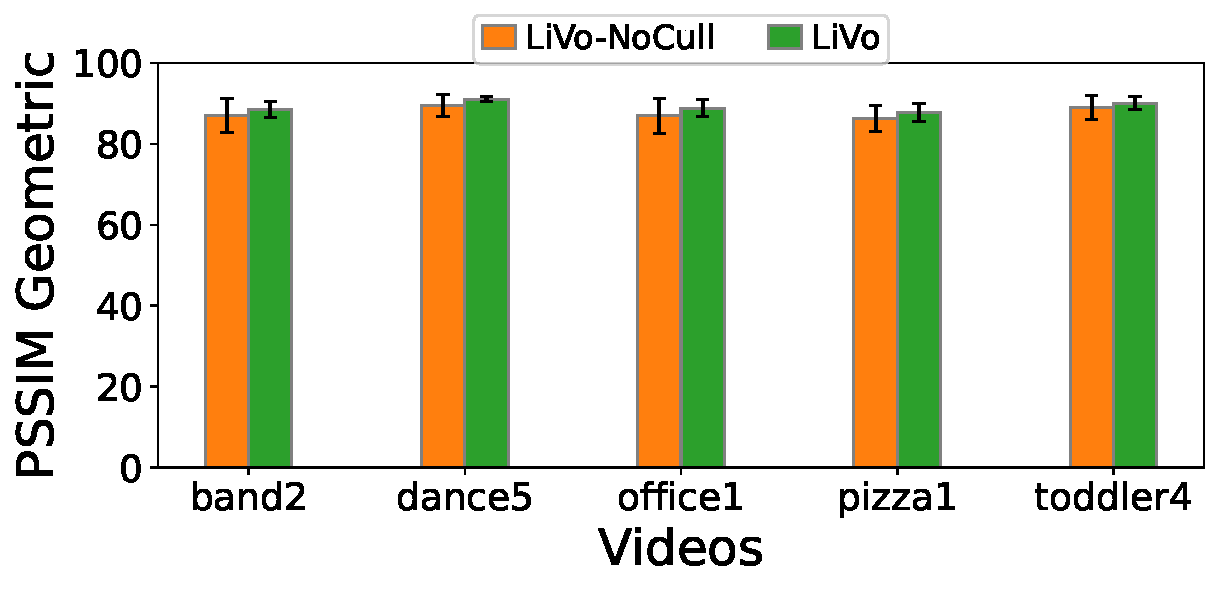
\includegraphics[width=\columnwidth]{figures/pssim_geo_without_stalls.pdf}
%   \caption{PSSIM discounting stalls.}
%   \label{plot:pssim_culling_imprv_quality}
% \end{figure}

\parab{Setup.}
%
%We now report on objective quality comparisons using PointSSIM (or PSSIM for short).
%
We use the same experimental setup as described above but now the receiver logs the received point cloud.
%
We compare each point cloud against ground truth for the same 5 videos, 3 user traces per video and 2 network traces.

\parab{Results.}
%
\cref{plot:pssim_geo_baselines} and \cref{plot:pssim_color_baselines} separately plot PSSIM for depth and color across 4 schemes.
%
For each video sequence, we aggregate the geometry and color PSSIM values over all user traces and network traces.
%
We use a metric value of 0 for frames that experience stalls.
%
Draco-Oracle achieves the lowest geometry and color score with mean value of $28.3$ (std. $19.1$) and $29.9$ (std. $19.8$) respectively, which correlates with the lower opinion scores in our user study.
%
%\textit{Dance5} achieves the highest score for Draco-Oracle; it also achieved the highest opinion score among the 5 videos (\cref{plot:study_videos}).

\livo outperforms \livo-NoCull, achieving a mean PSSIM geometry of $87.8$ (std. $3.7$) compared to $81.0$ (std. $9.5$) for \livo{}-NoCull.
%
This is consistent with our user study and demonstrates the benefits of culling.
%
\livo's benefits relative to \livo-NoCull are higher on videos with more subjects (\cref{tab:dataset-summary}); in such videos, users often focus on a few subjects at any given instant, so culling is very effective.
%
MeshReduce has significantly lower PSSIM geometry of $67.0$ (std. $1.8$) because it uses Draco, which is less bandwidth-efficient, and because it adapts indirectly to bandwidth.

\livo{} is slightly better than \livo{}-NoCull by the PSSIM color metric ($80.9$, std. $5.06$ vs. $82.9$, std. $7.59$).
%
This is because our bandwidth splitting allocates only a small fraction of available bandwidth to color, so any bandwidth reductions from culling for color are proportionally lower.
%
Interestingly, MeshReduce compares better with \livo{} for color ($77.30$, std. $10.6$).
%
We conjecture that in meshes, color is less affected by depth distortion than for point clouds.
%% This is in part because the decimation process recomputes surface color, but tries to approximate surface geometry well.
%% %
%% In \livo{}, distortion of a single pixel in the depth image can distort color, but this is less likely with meshes.

%% \raj{Do we need to talk about color? PSSIM color mean (std.) for Meshreduce, \livo-NoCull, and \livo are $80.9$ (std. $5.06$), $77.30$ (std. $10.6$), and $82.9$ (std. $7.59$), respectively. Meshreduce has higher PSSIM color is due to imbalance in the bandwidth apportioning. Maybe meshreduce provides adequate bandwidth to color than to geometry. Also, since mesh has consistent surface, even though geometry is bad perhaps the color of even unmatched points are fine, not like point cloud, where slight change in depth can produce mismatch in color. This is my hunch.}
%
%Moreover, the gap between performance of \livo and \livo-NoCull scheme on 4 videos, except \textit{dance5}, is higher. 
%
%These videos have more subjects (\cref{tab:dataset-summary}), so they demand higher bandwidth.
%
%In such videos, users often focus on a few subjects at any given instant, so culling becomes very effective to save bandwidth.

%While most of our results are consistent with the user study, by objective quality \livo surprisingly outperforms \livo-NoCull for toddler4, though study participants thought otherwise.
%
%This means that participants were put off by prediction artifacts which mask the benefits of quality, but these artifacts did not impact PointSSIM.

Stalls impact objective quality, and \cref{plot:stalls} shows the aggregate stalls across videos for 3 schemes.
%
We omit MeshReduce since it doesn't experience stalls: it uses reliable transmissions and its parameters are designed to match average bandwidth, so rather than stalls it exhibits varying frame rates.
%
Draco-Oracle suffers from high mean stall rate of $69.3\%$.
%
Even on the \textit{dance5} video which has only 1 participant and no objects in the scene (\cref{tab:dataset-summary}), it has a stall rate of $37.8\%$.
%
%The stalls increase significantly with increase in number of subjects or objects in the scene.
%
\livo-NoCull incurs an average stall rate of $7.9\%$ (std. $7.5\%$) while \livo incurs $1.7\%$ (std. $2.3\%$); culling accounts for this difference.
%
\livo's infrequent stalls occur when the rate-adaptive codec overshoots the bandwidth target.

%\harsha{Drop para below for space?}
Culling by itself improves quality: \livo improves over \livo-NoCull by an average difference of $2\%$ for PSSIM geometry (\cref{plot:pssim_culling_imprv_quality}) and $1\%$ for color (omitted for brevity).

Overall, both by objective and perceptual measures, \livo{} consistently outperforms all baselines for our videos.
%\ramesh{Raj, either add a graph of PSSIM per bandwidth trace. Or, we can leave it out, but please check the following para.}
%% Overall, \livo achieves a PSSIM of 80-90 for geometry and slightly less for color.
%% %
%% As expected, these values are higher for \textit{trace-1} with a higher bandwidth (graph omitted for brevity).
%\sanjay{Why does LiVo have stalls if it is live conferencing? Wouldn't it just skip? Also right most graph (Fig 10) says "No Stalls" and isn't discussed. What does "No Stalls" mean here (are there 2 settings of these systems, one with stalls and one without?) Is the last graph Color or Geometry? }

\subsection{Performance Validation}
\label{s:perf-valid}

\begin{comment}
\parab{Outline.}
Plot graph of end-to-end latency. Discuss per component latency.

Plot graph showing FPS achieved. Discuss the results. This can be brief, since there may not be much to say, unless there are significant dips.
\end{comment}

% \begin{figure}[t]
% 	\centering 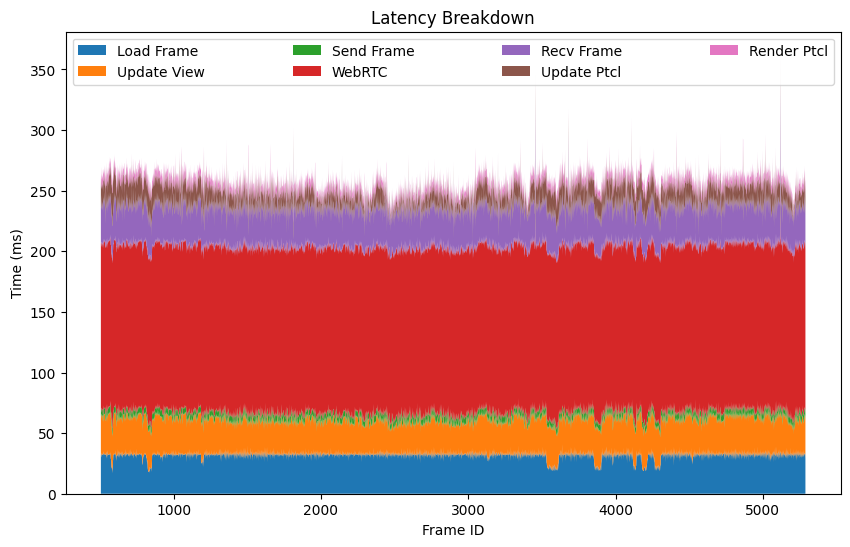
\includegraphics[width=\columnwidth]{figures/e2e_latency.png}
% 	\caption{End-to-end latency breakdown. \raj{Table or figure?}}
% 	\label{plot:latency}
% \end{figure}

%\begin{table}[t]
%\centering
%  \footnotesize
%    \begin{tabular}{|l|l|l|l|l|}
%    \hline
%    \multicolumn{1}{|l|}{\multirow{2}{*}{\textbf{Component}}} & \multicolumn{2}{c|}{\textbf{LiVo-NoCull (in ms)}} & \multicolumn{2}{c|}{\textbf{LiVo (in ms)}} \\ \cline{2-5} 
%    \multicolumn{1}{|l|}{} & \multicolumn{1}{l|}{\textbf{Mean}} & \multicolumn{1}{l|}{\textbf{Std}} & \multicolumn{1}{l|}{\textbf{Mean}} & \multicolumn{1}{l|}{\textbf{Std}} \\ \hline
%    View Generation & 14.75 & 2.48 & 26.31 & 3.01 \\ \hline
%    Tile Creation & 6.83 & 1.85 & 7.71 & 2.45 \\ \hline
%    \begin{tabular}[c]{@{}l@{}}Point cloud\\ reconstruction\end{tabular} & 12.64 & 2.28 & 11.82 & 3.44 \\ \hline
%    Rendering & 8.42 & 2.74 & 4.27 & 1.50 \\ \hline
%    WebRTC Send-Recv & 239.35 & 4.54 & 236.05 & 2.84 \\ \hline
%    \textbf{Total latency} & \textbf{281.99} & \textbf{6.93} & \textbf{286.17} & \textbf{8.12} \\ \hline
%    \end{tabular}
%    \caption{Component-wise latency. \note{[Old]}}
%    \label{tab:latency}
%\end{table}

\begin{table}[t]
\centering
% \footnotesize
    % \scalebox{0.8}
    {
	\begin{tabular}{|l|l|l|l|l|}
		\hline
		\multicolumn{1}{|l|}{\multirow{2}{*}{\textbf{Component}}} & \multicolumn{2}{c|}{\textbf{\livo-NoCull (in ms)}} & \multicolumn{2}{c|}{\textbf{\livo (in ms)}} \\ \cline{2-5} 
		\multicolumn{1}{|l|}{} & \multicolumn{1}{l|}{\textbf{Mean}} & \multicolumn{1}{l|}{\textbf{Std}} & \multicolumn{1}{l|}{\textbf{Mean}} & \multicolumn{1}{l|}{\textbf{Std}} \\ \hline
		Capture Frame 						& 32.75 & 6.81  & 29.85 	& 5.09 \\ \hline
		View Generation 					& 19.50 & 8.93 & 30.59 	& 2.91 \\ \hline
		Tile Creation 						& 7.16 & 5.08 & 5.49  	& 0.86 \\ \hline
		Synchronization						& 31.74 & 14.24 & 32.33	& 4.60 \\ \hline
		% \begin{tabular}[c]{@{}l@{}}
		% 	Point cloud\\ Reconstruction
		% \end{tabular} 
            Point cloud Reconstruction & 21.80 & 2.47 & 15.83 	& 3.64 \\ \hline
		Rendering 							& 5.16 & 1.32 & 4.91  	& 1.23 \\ \hline
		WebRTC Send-Recv 					& 133.19 & 2.13 & 132.82	& 0.65 \\ \hline
		\textbf{Total latency} 				& \textbf{251.30} & \textbf{23.32} & \textbf{251.82} & \textbf{6.93} \\ \hline
	\end{tabular}
    }
	\caption{Component-wise latency.} % Band2 video
	\label{tab:latency}
\end{table}

\cref{tab:latency} lists the per-component latency for \livo and \livo-NoCull.
%
Both achieve end-to-end latency within 300~ms, in line with production 2D video conferencing systems such as Zoom, Meet, \etc~\cite{videoconf-benchmark, salsify}.
%
For \livo, the sender processing latency is around 64~ms while the receiver processing latency is 53~ms.
%
In contrast, \livo-NoCull incurs lower processing latency at the sender since it does not perform view culling, but incurs the culling cost at the receiver.
%
The largest latency is incurred by WebRTC transmission (color and depth transmissions are parallel), which is about 137~ms.
%
Much of this is attributable to the jitter buffer in WebRTC: we use 100~ms~\cite{jitterbuffer-imc2023}, consistent with current practice.
%
%\livo also incurs an additional overhead of 200~ms, not included in~\cref{tab:latency}, due to an implementation artifact.
%
%Most of \livo is in C++, except the gstreamer WebRTC component which is in Python, and this latency in incurred in handing off frames to the Python component.
%
%This also explains why the WebRTC component is slow; we plan to convert it in the future to C++ to optimize the implementation end-to-end.

\begin{figure}[t]
	\begin{minipage}[t]{0.49\columnwidth}
		\centering
		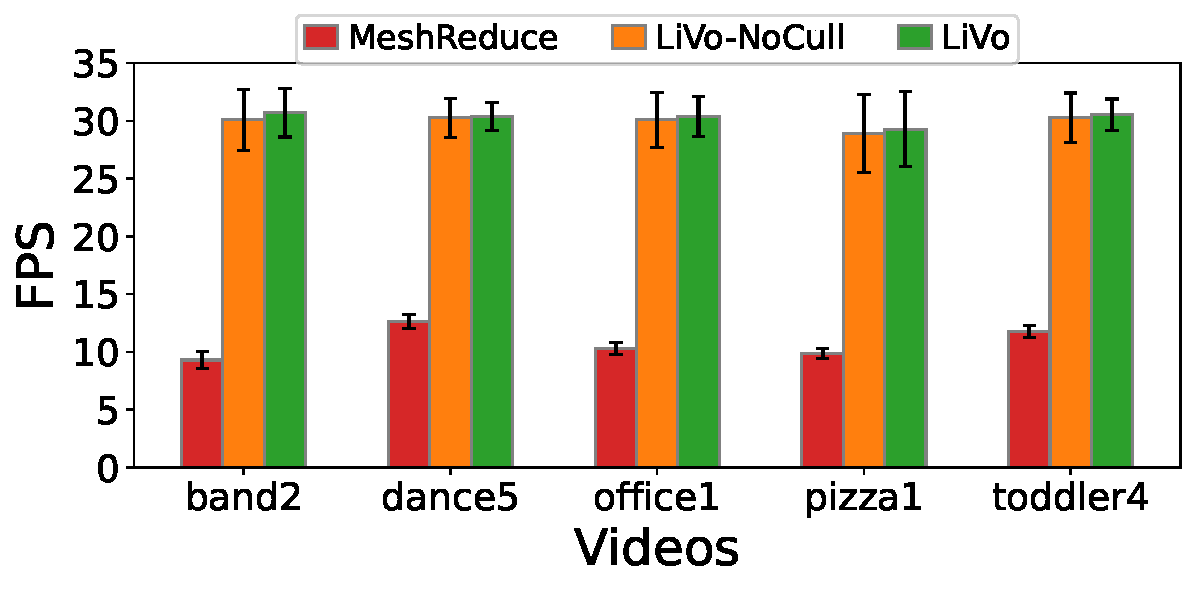
\includegraphics[width=\columnwidth]{figures/fps_tracep1.pdf}
		\caption{FPS comparison for \textit{trace-1}.}
		\label{plot:fps_tracep1}
	\end{minipage}
	\begin{minipage}[t]{0.49\columnwidth}
		\centering
		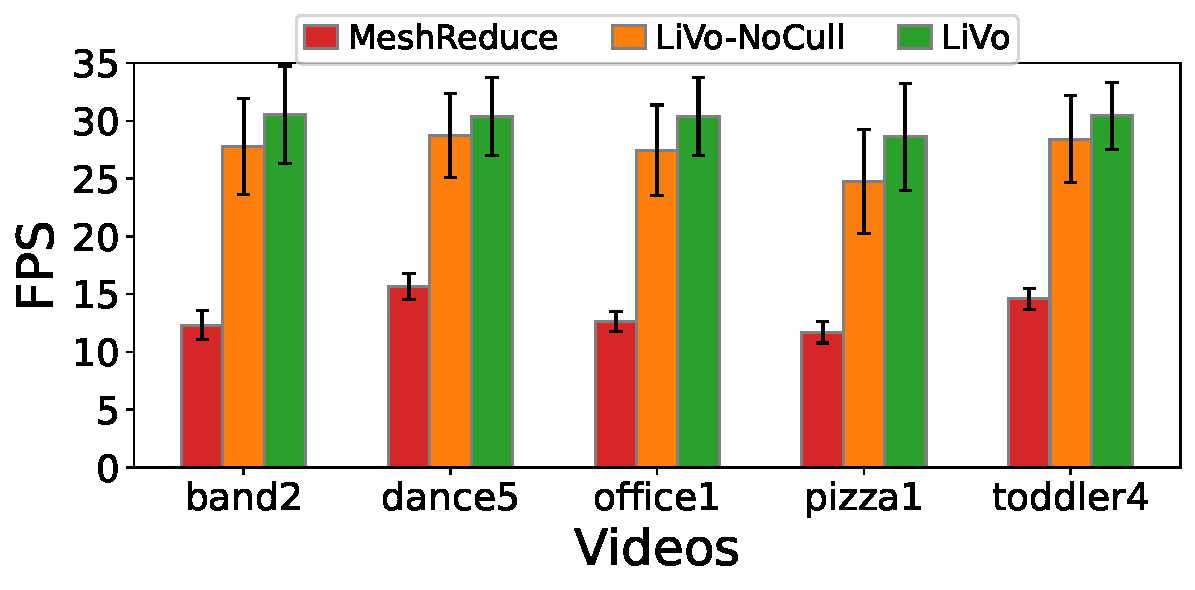
\includegraphics[width=\columnwidth]{figures/fps_wifi-25.pdf}
		\caption{FPS comparison for \textit{trace-2}.}
		\label{plot:fps_wifi25}
	\end{minipage}
\end{figure}

\cref{plot:fps_tracep1} plots the rendering frame rate for \livo-NoCull and \livo for \textit{trace-1}.
%
\livo maintains 30~fps at a lower standard deviation than \livo-NoCull.
%
For \textit{trace-2} (\cref{plot:fps_wifi25}), \livo maintains close to 30~fps (std. 0.7), while \livo-NoCull achieves 28~fps (std. 1.8).
%
At lower bandwidth, \livo-NoCull experiences more stalls (mean fps drops to 24~fps for \textit{pizza1}) than \livo, as compressed frames occasionally exceed the bandwidth budget.
%
MeshReduce achieves a mean frame rate of 12.1~fps, 2.5x lower than \livo, even though it utilizes all cores on the sender side at 100\% to encode frames.
%
MeshReduce's frame rate for \textit{trace-2} is slightly higher than \textit{trace-1}, because it decimates the mesh more to fit the lower bandwidth, and the encoder needs to do less work.
%
MeshReduce has been shown to outperform LiveScan3D~\cite{livescan3d} and Holoportation~\cite{holoportation}, so we have not included these in our evaluation.

%Overall, \livo outperforms most of the competitors in \cref{tab:comparison}.

% \subsection{Validating Design Choices}
% \label{s:valid-design-choic}

% \cref{s:just-design-choic} describes experiments that justify our design choices. Our key findings are:
% \begin{itemize}
% \item \livo{}'s dynamic bandwidth splitting is always within 0.5 in depth and 3 in color PSSIM of the best static split, even in bandwidth-constrained settings.
% \item \livo{}'s scaled depth encoding has color and geometry PSSIM over 90, ie better than the unscaled version, and better than prior work~\cite{realsense-doc,depth-kautz,vrcomm}.
% \item \livo{}-NoAdapt, a version of \livo{} without bandwidth adaptation and culling has 30-41\% lower geometry PSSIM and 27-37\% lower color PSSIM than \livo{}.
% \item Its frustum prediction guard-band of 20~cm finds the sweet-spot between accuracy and data reduction.
% \item Its frustum predictor is significantly more accurate than an MLP trained using a few traces.
% \end{itemize}

\subsection{Validating Design Choices}\label{s:just-design-choic}

\parab{Depth Encoding.}
\begin{figure}[t]
  \centering 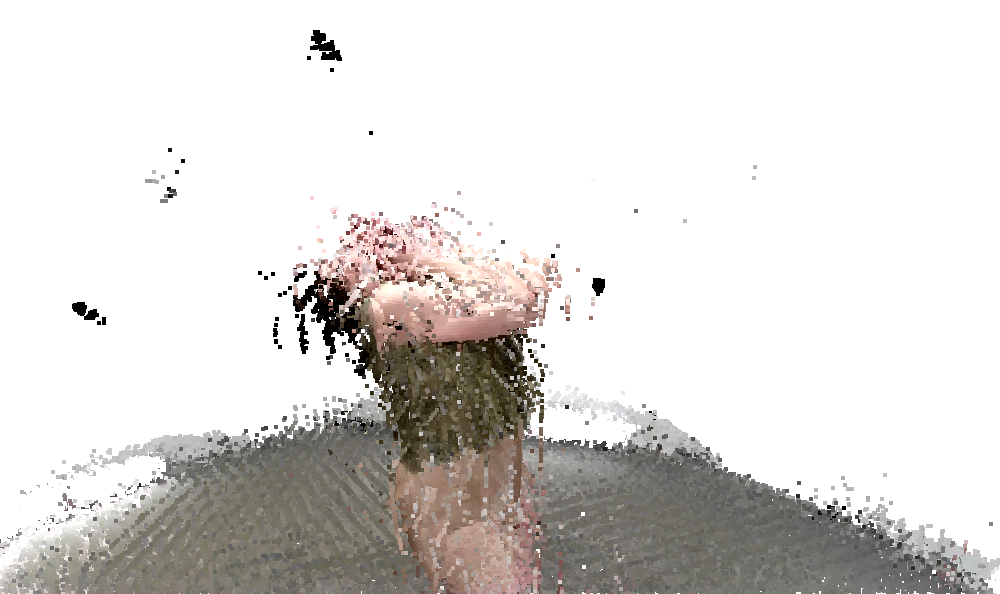
\includegraphics[width=0.8\columnwidth]{figures/depth_unscaled_artifact.png}
  \caption{Block artifacts arising from unscaled depth encoding when we use naive H.265 YUV 16-bit variant.}
  \label{fig:depth-unscaled-artifact}
\end{figure}
%
\livo encodes in Y-channel (luminance) of 3 channel 16-bit variant of H.265 encoding (Y444\_LE).
%
If the depth values aren't scaled to the full range, they produce artifacts as seen in \cref{fig:depth-unscaled-artifact}.
%
These artifacts arise since nearby depth values are mapped to same quantization bin within the 16-bit range.
%
So \livo scales the depth values.
%
We also experimented with a strategy proposed by prior work~\cite{realsense-doc,depth-kautz,vrcomm} which colorizes each 16-bit depth pixel into a 3-channel RGB pixel using a depth to color conversion table.
%
\cref{plot:compression-choice} shows that \livo{}'s scaled depth encoding achieves the highest geometry and color PSSIM relative to this approach and to unscaled depth encoding.

%% is significantly better than encoding depth in RGB, and that depth scaling is necessary to improve quality.
% %
% When we implement this strategy inside \livo and apply to \textit{dance5} video, the average PointSSIM quality drops below 20 for both color and depth, which indicates severe quality degradation.
% %
% In contrast, naive strategy of putting depth in Y-channel (luminance) of 3 channel 16-bit variant of H.265 encoding (Y444\_LE Unscaled), improves PointSSIM geometry to above $70$.
% %
% Through visual inspection, we observed that the decoded point cloud have local block-like artifacts, which indicates that the neighbouring points have collapsed in one of the 3D dimensions (example in Appendix \cref{s:appendix}).
% %
% Our depth encoding strategy using depth scaling improves both PointSSIM color and geometry to reach 90.

\begin{figure}[tbp]
  \centering 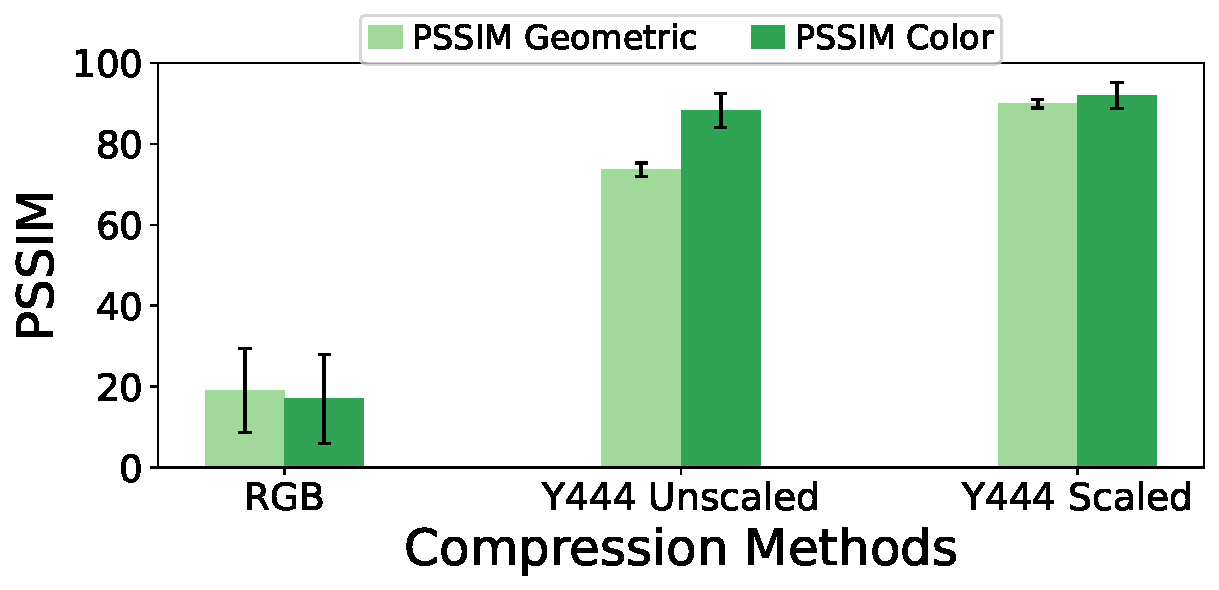
\includegraphics[width=0.6\columnwidth]{figures/pssim_compression_comparison.pdf}
  \caption{Comparison between realsense vs our approach.}
  \label{plot:compression-choice}
\end{figure}

%\harsha{Suggest moving the para below and associated table to appendix.}
\parab{Kalman Filter buffer size.}
%
Kalman filter prediction error depends on the prediction horizon.
%
\livo targets prediction horizons of about 10 frames (300~ms).
%
Predictions help culling, which can reduce data volume, but erroneous predictions can impact quality.
%
\livo uses a static guard-band $\epsilon$ of 20~cm around the frustum to minimize quality loss due to prediction errors.
%
\cref{tab:prediction_acc} shows that for guard-bands up to 30~cm, \livo's accuracy and data volume are relatively insensitive to the choice of guard-band, hence a static guard-band works well.
%
We have verified this for other videos as well.

% Prediction window is the number of lookahead frames between the last received frustum from receiver and the frustum required (through prediction) for the current outgoing frame on the sender.
% %
% We predict the frustum by running the Kalman Predictor same number of times as the prediction window size.
% %
% To correct for prediction errors, we use a guard band $\epsilon$ around the predicted frustum.
% %
% \cref{tab:prediction_acc} shows that for any prediction window size, the prediction accuracy increases with increase in the guard band size, but it comes at a cost.
% %
% Increased size of guard band results in large fraction of points in the full point cloud to fall inside the frustum; refer~\cref{tab:prediction_fraction}.
% %
% This increases unnecessary transmission of data at reduced quality.
% %
% We observe that \livo achieves an end-to-end latency <300~ms, which corresponds to a prediction window size of 10 frames (at 30~FPS).
% %
% From \cref{tab:prediction_acc}, we observe that increasing guard band size above 20~cm have marginal improvements in prediction accuracy, while saving $40\%$ of the points from transmission.
% %
% Thus, we choose $\epsilon$ to be 20~cm in \livo.

\begin{table}[t]
\centering
  \footnotesize
  % \scalebox{0.8}{
    \begin{tabular}{|l|l|l|l|l|}
    \hline
    \multicolumn{1}{|l|}{\multirow{2}{*}{\textbf{\begin{tabular}[c]{@{}l@{}}Guard \\ Band\end{tabular}}}} & \multicolumn{4}{c|}{\textbf{Prediction Window Size}} \\ \cline{2-5} 
    \multicolumn{1}{|l|}{} & \multicolumn{1}{l|}{\textbf{W=5}} & \multicolumn{1}{l|}{\textbf{W=10}} & \multicolumn{1}{l|}{\textbf{W=20}} & \multicolumn{1}{l|}{\textbf{W=30}} \\ \hline
    10 & 98.44 (0.57) & 96.69 (0.54) & 94.37 (0.57) & 91.76 (0.57) \\ \hline
    20 & 99.26 (0.62) & 98.37 (0.62) & 96.13 (0.62) & 93.95 (0.62) \\ \hline
    30 & 99.61 (0.66) & 98.97 (0.66) & 97.22 (0.67) & 95.41 (0.67) \\ \hline
    50 & 99.89 (0.73) & 99.56 (0.73) & 98.46 (0.73) & 97.18 (0.73) \\ \hline
    \end{tabular}
    % }
    \caption{Accuracy  of culling using Kalman Filter by varying the guard band (in cm) for \textit{band2}. The numbers in brackets represent fraction of points within frustum.}
    \label{tab:prediction_acc}
\end{table}

% \begin{table}[t]
% \centering
%   \footnotesize
%     \begin{tabular}{|l|l|l|l|l|}
%     \hline
%     \multicolumn{1}{|l|}{\multirow{2}{*}{\textbf{\begin{tabular}[c]{@{}l@{}}Guard Band\\ (in cm)\end{tabular}}}} & \multicolumn{4}{c|}{\textbf{Prediction Window Size}} \\ \cline{2-5} 
%     \multicolumn{1}{|l|}{} & \multicolumn{1}{l|}{W=5} & \multicolumn{1}{l|}{W=10} & \multicolumn{1}{l|}{W=20} & \multicolumn{1}{l|}{W=30} \\ \hline
%     10 & 0.57 & 0.54 & 0.57 & 0.57 \\ \hline
%     20 & 0.62 & 0.62 & 0.62 & 0.62 \\ \hline
%     30 & 0.66 & 0.66 & 0.67 & 0.67 \\ \hline
%     50 & 0.73 & 0.73 & 0.73 & 0.73 \\ \hline
%     \end{tabular}
%     \caption{Fraction of points within the frustum by varying guard band size for `band2' video.}
%     \label{tab:prediction_fraction}
% \end{table}

% \begin{figure}[t]
%  \begin{minipage}[t]{0.49\columnwidth}
%    \centering
%     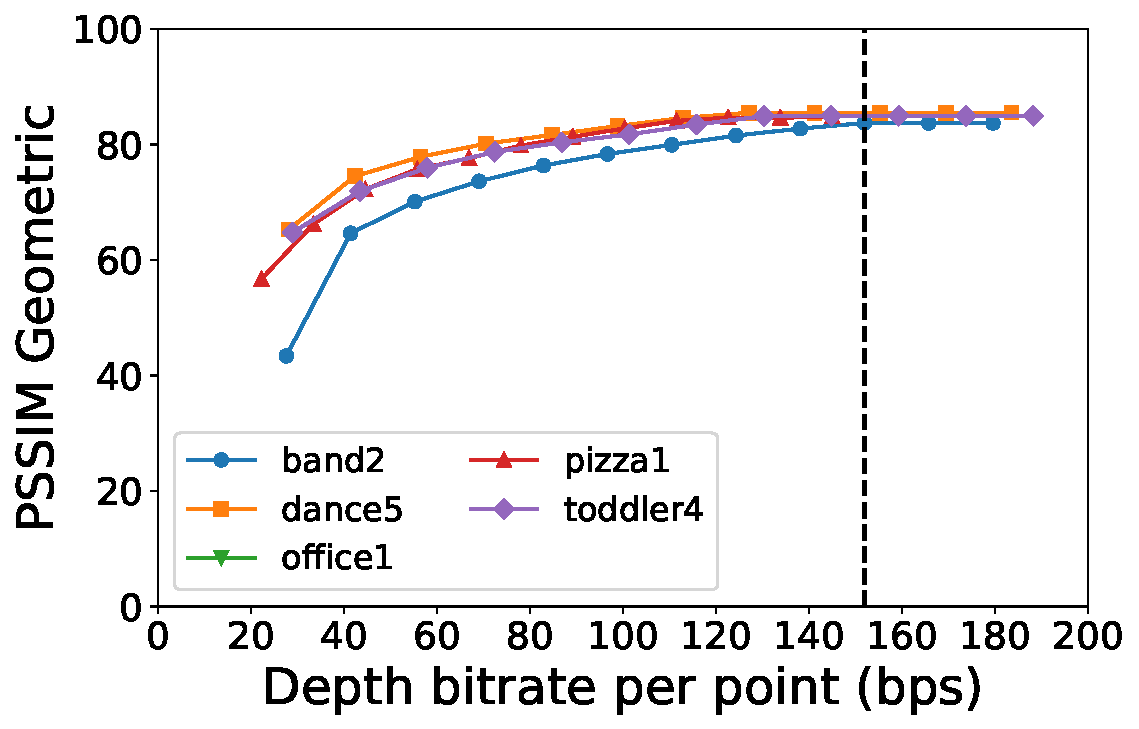
\includegraphics[width=\columnwidth]{figures/pssim_geometric_depth_per_point.pdf}
%    \caption{Depth distortion. \note{[Remove]}}
%    \label{plot:depth-distortion}
%  \end{minipage}
%  \begin{minipage}[t]{0.49\columnwidth}
%    \centering
%     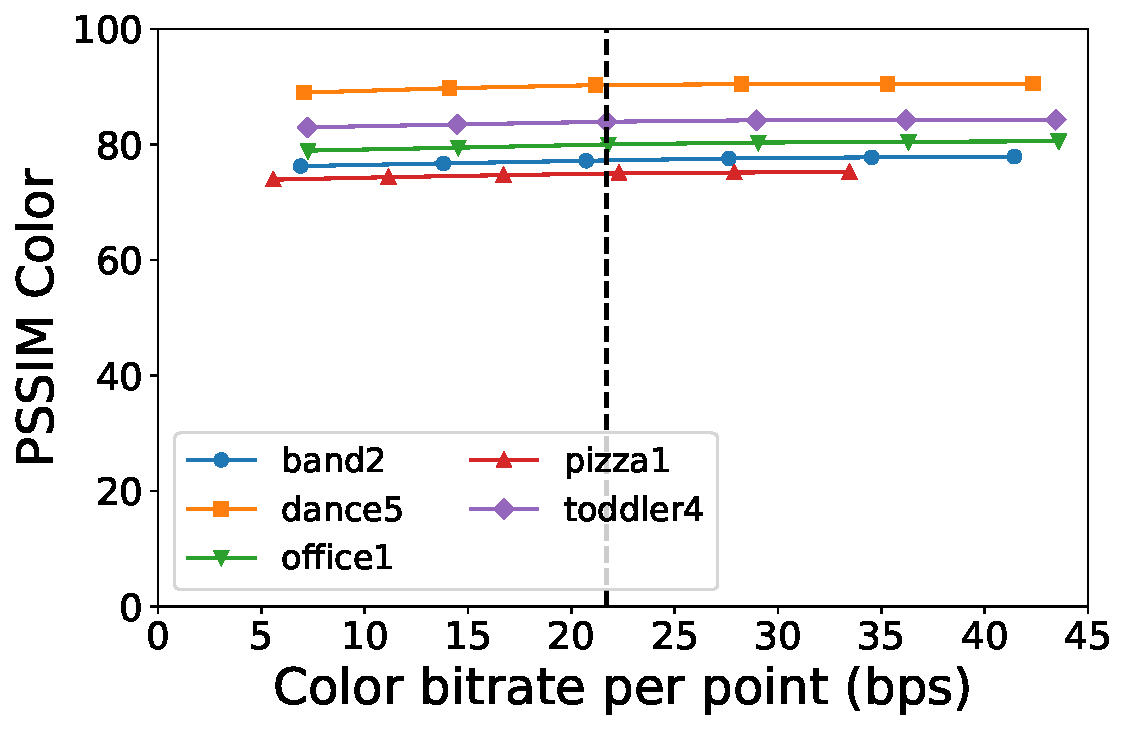
\includegraphics[width=\columnwidth]{figures/pssim_color_color_per_point.pdf}
%    \caption{Color distortion. \note{[Remove]}}
%    \label{plot:color-distortion}
%  \end{minipage}
% \end{figure}

\begin{figure}[t]
  \begin{minipage}[t]{0.49\columnwidth}
	    \centering
	     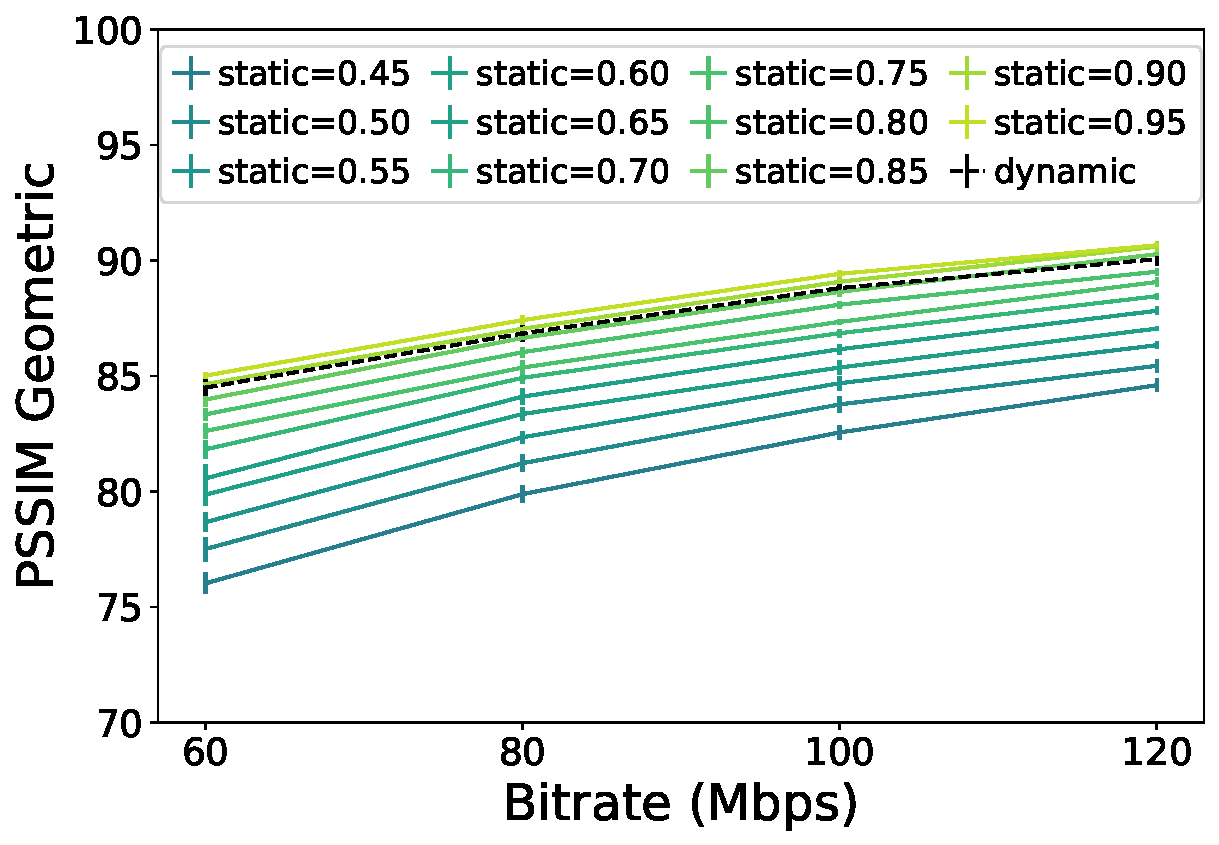
\includegraphics[width=\columnwidth]{figures/static_vs_dynamic_pssim_geo.pdf}
	    \caption{PSSIM Geometric for static vs dynamic split.}
	    \label{plot:split-sweep-geo}
	  \end{minipage}
  \begin{minipage}[t]{0.49\columnwidth}
	    \centering
	     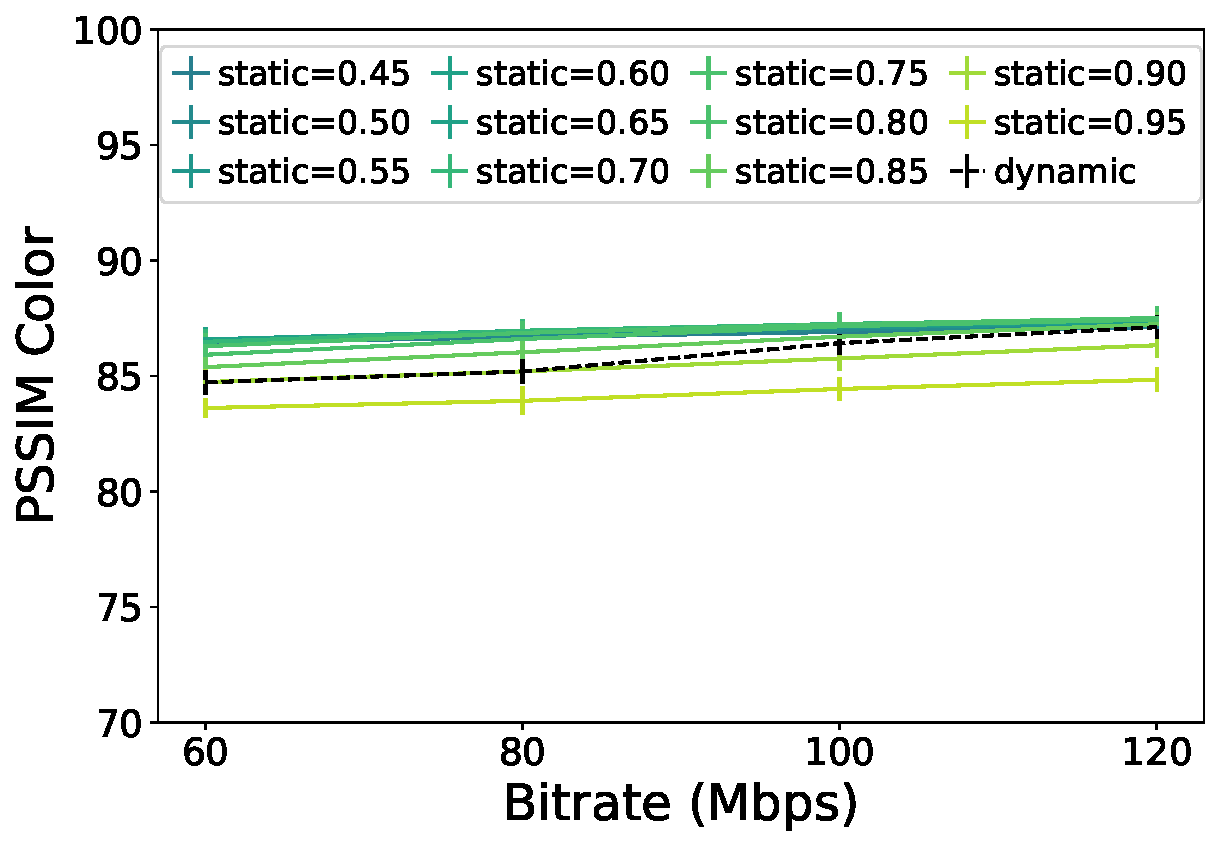
\includegraphics[width=\columnwidth]{figures/static_vs_dynamic_pssim_color.pdf}
	    \caption{PSSIM Color for static vs dynamic split.}
	    \label{plot:split-sweep-color}
	  \end{minipage}
\end{figure}

%% \begin{figure}[t]
%% 	\centering 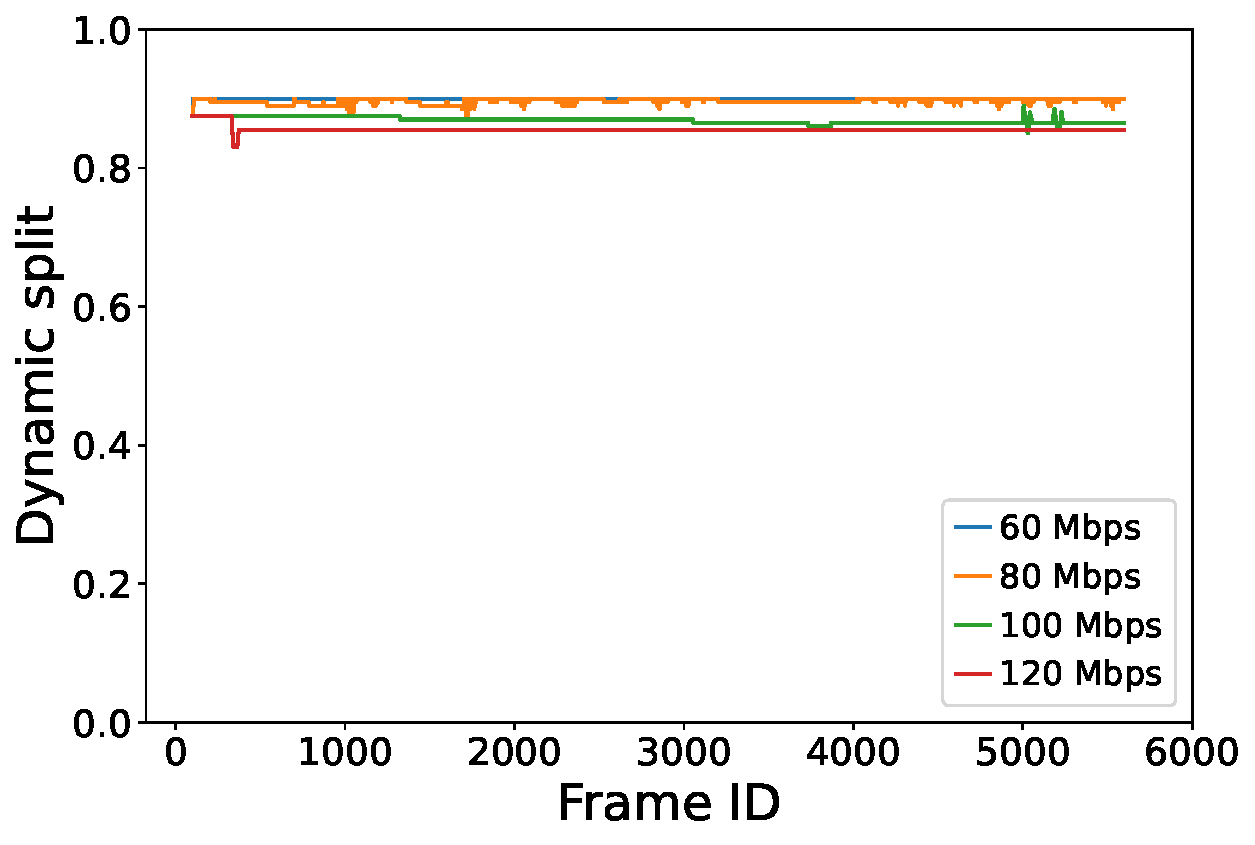
\includegraphics[width=0.5\columnwidth]{figures/split_convergence.pdf}
%% 	\caption{Split convergence.}
%% 	\label{plot:split-convergence}
%% \end{figure}

\parab{Bandwidth Splitting.}
%
%\cref{plot:depth-distortion} plots depth PSSIM as a function of bits per second per point, when color is assigned a high (100~Mbps) rate.
%
%Across all our videos, depth quality saturates at about 152 bits per second per point.
%
%Conversely, when depth bit rate is fixed, color PSSIM saturates at about 22 bits per second (\cref{plot:color-distortion}).
%
%Perceptual quality in 3D is more sensitive to depth encoding than color, since loss in depth leads to geometrical errors that can distort a 3D representation of an object.
%
%This justifies our choice of 7:1 as the ratio of depth to color per point.
%
\cref{plot:split-sweep-geo} plots compares PSSIM for different static splits with \livo{}'s dynamic split (\cref{ss:bw-adaptation}) for bitrates ranging from 60-120~Mbps for \textit{office1} (similarly, color in \cref{plot:split-sweep-color}).
%
Dynamic splitting is with 0.5 PSSIM points for geometry and 3 PSSIM points for color relative to the best static split.
%
As available bandwidth increases, both geometry and color PSSIM values are within 0.5 of the best static split.
%
This demonstrates the effectiveness of dynamic splitting.
%
%% \cref{plot:split-convergence} shows how quickly the bitrate split converges when the scene complexity changes. 
%
Moreover, dynamic splitting converges quickly, within 5-10 frames (figure omitted for brevity).
%
%Also, the split variation occurs more for bandwidth limited than bandwidth adequate regions.
%

\parab{Bandwidth Adaptation.}
%
% \begin{figure}[t]
%      \centering
%      \begin{subfigure}[b]{0.49\columnwidth}
%          \centering
%          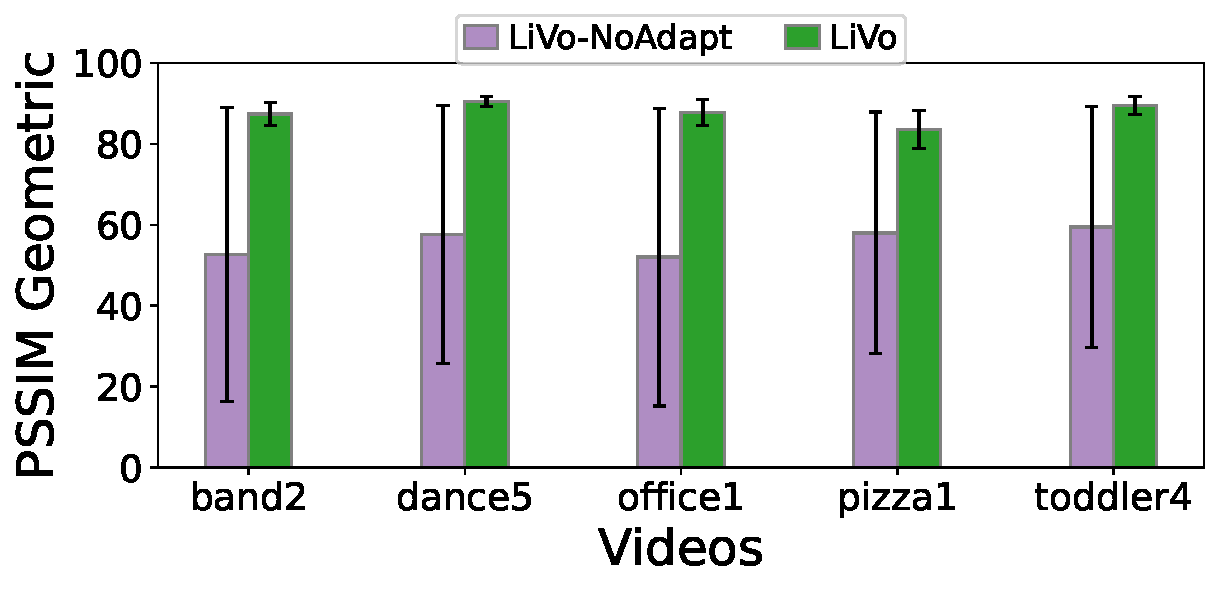
\includegraphics[width=\columnwidth]{figures/pssim_geo_starline_livo.pdf}
%          \caption{Geometry}
%          \label{plot:pssim_geo_starline_livo}
%      \end{subfigure}
%      \hfill
%      \begin{subfigure}[b]{0.49\columnwidth}
%          \centering
%          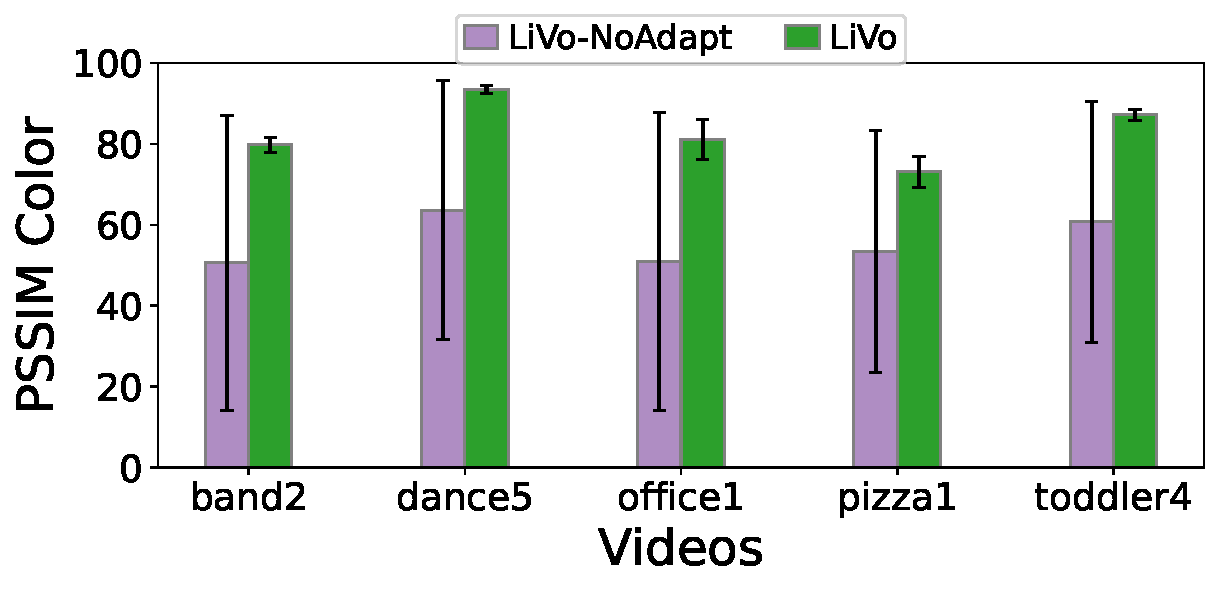
\includegraphics[width=\columnwidth]{figures/pssim_color_starline_livo.pdf}
%          \caption{Color}
%          \label{plot:pssim_color_starline_livo}
%      \end{subfigure}
%     \caption{PSSIM metric for Starline (no adaptation) vs \livo}
%     \label{plot:pssim_starline_livo}
% \end{figure}
%
\begin{figure}[t]
  \begin{minipage}[t]{0.49\columnwidth}
    \centering
     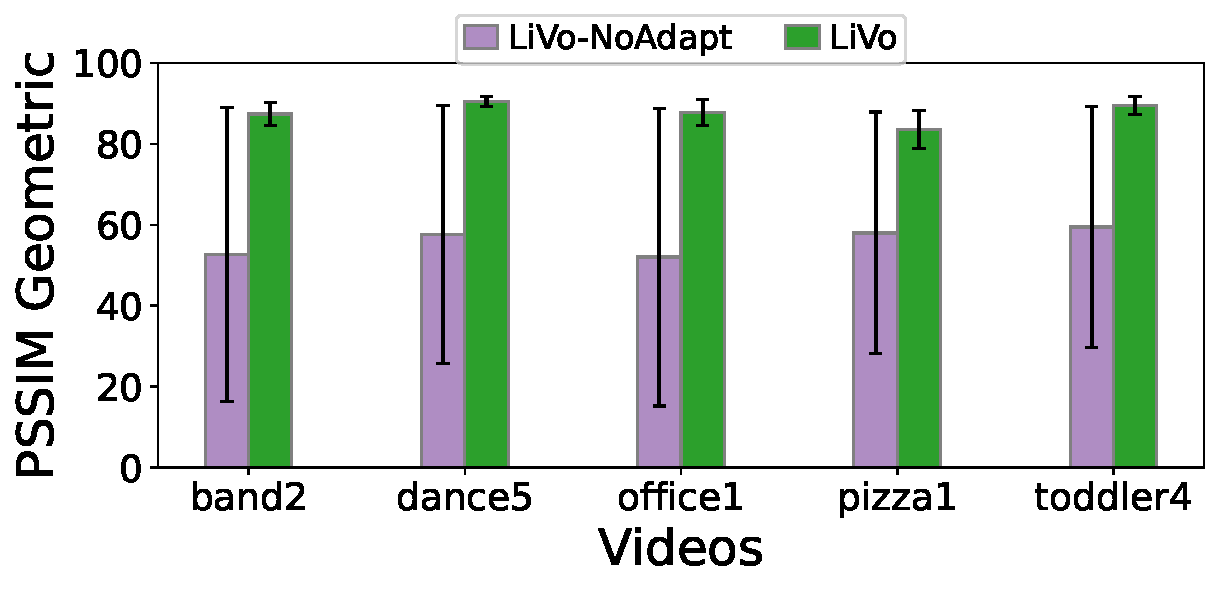
\includegraphics[width=\columnwidth]{figures/pssim_geo_starline_livo.pdf}
    \caption{PSSIM Geometric, \livo-NoAdapt vs \livo.}
    \label{plot:pssim_geo_starline_livo}
  \end{minipage}
  \begin{minipage}[t]{0.49\columnwidth}
    \centering
     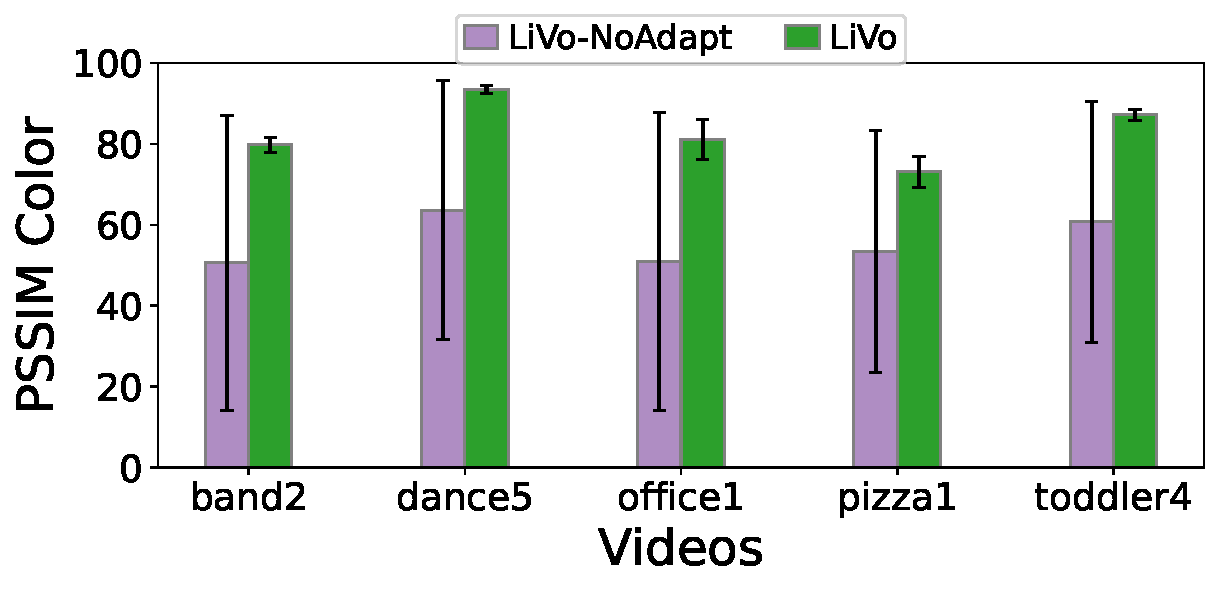
\includegraphics[width=\columnwidth]{figures/pssim_color_starline_livo.pdf}
    \caption{PSSIM Color, \livo-NoAdapt vs \livo.}
    \label{plot:pssim_color_starline_livo}
  \end{minipage}
\end{figure}
%
What if LiVo did not use bandwidth-adaptation and view culling at all, but instead used fixed quality parameters?
%
We set fixed color QP (quantization parameter) to 22 and depth QP to 14; Starline~\cite{starline} uses these values.
%
\cref{plot:pssim_geo_starline_livo} and \cref{plot:pssim_color_starline_livo} show that this LiVo-NoAdapt has significant quality drop of $30-41\%$ for geometry and $27-37\%$ for color, with PSSIM going below 60.

\parab{Frustum Prediction.}
%
\begin{table}[t]
\centering
\footnotesize
    % \scalebox{0.8}
    % {
	\begin{tabular}{|l|l|l|l|}
		\hline
		\textbf{Method} & \textbf{\begin{tabular}[c]{@{}l@{}}\# Hidden \\ Units\end{tabular}} & \textbf{\begin{tabular}[c]{@{}l@{}}Position \\ (m)\end{tabular}} & \textbf{\begin{tabular}[c]{@{}l@{}}Rotation \\ (degree)\end{tabular}} \\ \hline
		\multirow{3}{*}{\begin{tabular}[c]{@{}l@{}}MLP\\ Trained on \\ 1 user trace\end{tabular}} & 3 & 1.01 & 135.86 \\ \cline{2-4} 
		& 32 & 0.59 & 80.46 \\ \cline{2-4} 
		& 64 & 0.24 & 58.24 \\ \hline
		\multirow{3}{*}{\begin{tabular}[c]{@{}l@{}}MLP\\ Trained on\\ 2 user trace\end{tabular}} & 3 & 0.40 & 33.34 \\ \cline{2-4} 
		& 32 & 0.09 & 3.69 \\ \cline{2-4} 
		& 64 & 0.07 & 2.17 \\ \hline
		Kalman Filter & - & 0.04 & 7.19 \\ \hline
	\end{tabular}
    % }
	\caption{Comparing prediction errors in Kalman Filter-based to learning-based prediction methods.} % For band2 video
	\label{tab:frustum_kf_learning}
\end{table}
%
To estimate quality impairment as a result of our predictive culling, we compare it against LiVo with perfect culling (using predictions obtained from the user trace).
%
The average quality difference in PSSIM geometry and color is $1\%$ across all 5 videos when run on \textit{trace-1}.

Prior work has trained frustum predictors from user traces~\cite{vues,vivo} for on-demand volumetric videos.
%
This doesn't quite apply to conferencing, since user interactions depend on content, which can be different for different content.
%
That said, we evaluate (\cref{tab:frustum_kf_learning}) whether an MPL with 3 hidden layers used in ViVo~\cite{vivo} could learn from a small number of our traces.
%
We find that it may be possible to match LiVo's predictor only with a large number of hidden layers (64); with the three that ViVo uses, prediction errors are unacceptably high.


% \begin{figure}[t]
%      \centering
%      \begin{subfigure}[b]{0.9\columnwidth}
%          \centering
%     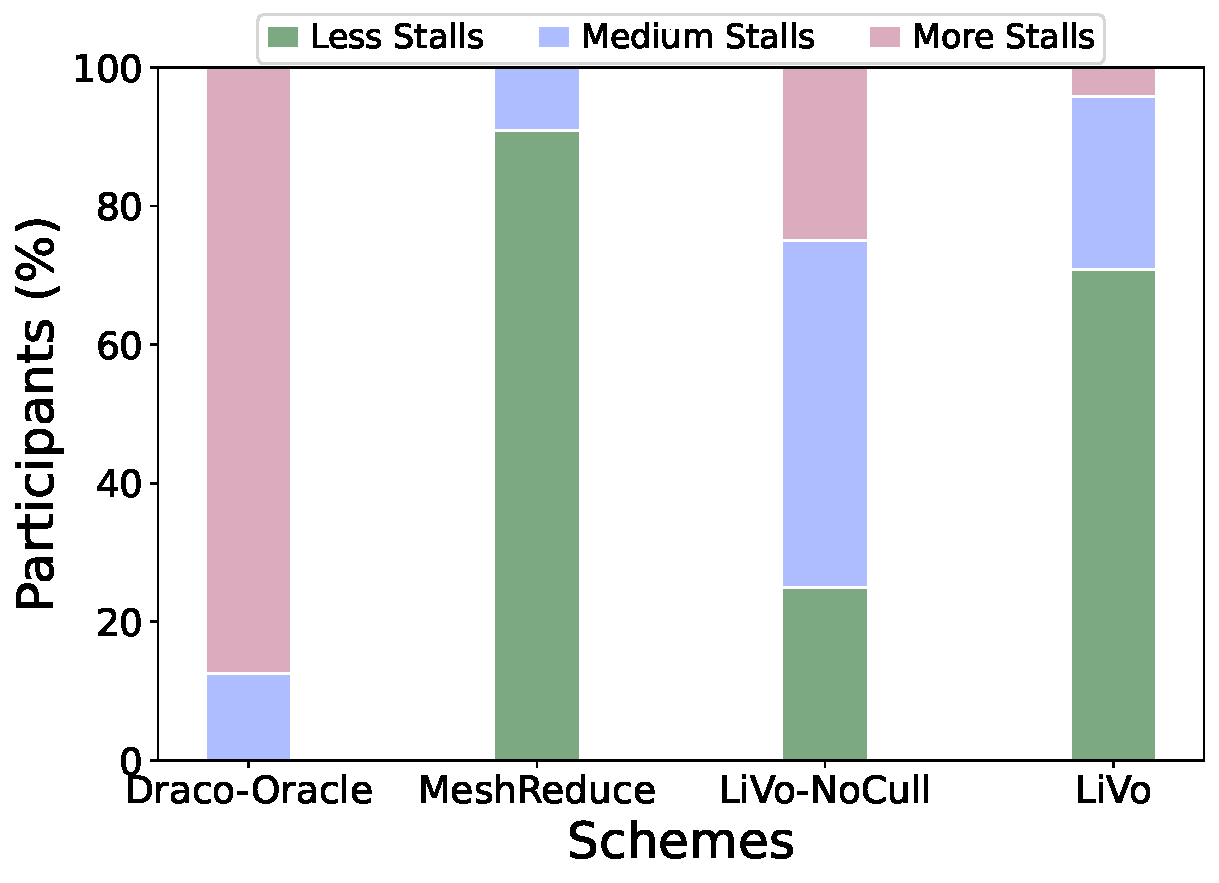
\includegraphics[width=\columnwidth]{figures/user_study_stall_distribution.pdf}
%     \caption{Feedback on stalls}
%     \label{plot:user_study_stalls}
%      \end{subfigure}
%      \hfill
%      \begin{subfigure}[b]{0.9\columnwidth}
%          \centering
%          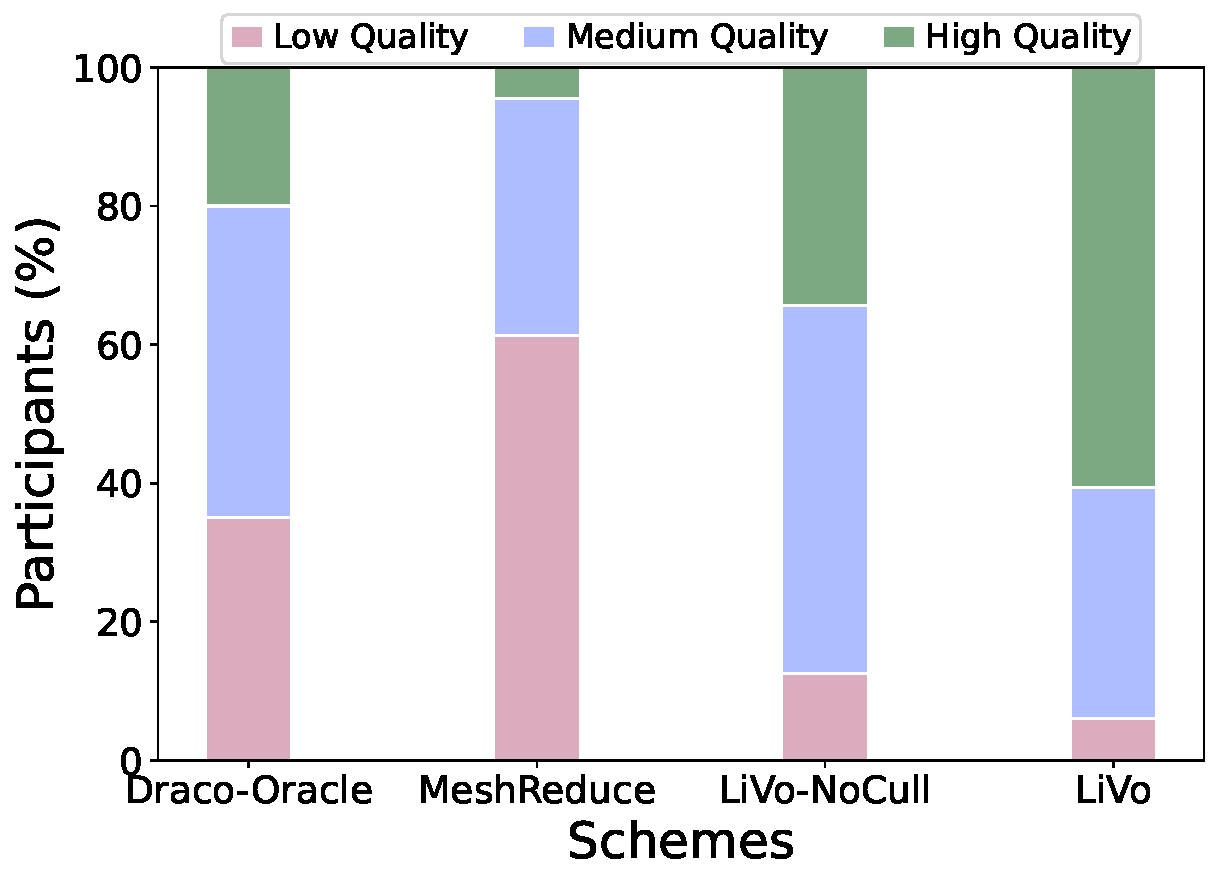
\includegraphics[width=\columnwidth]{figures/user_study_quality_distribution.pdf}
%     \caption{Feedback on quality.}
%     \label{plot:user_study_quality}
%      \end{subfigure}
%      \hfill
%      \begin{subfigure}[b]{0.9\columnwidth}
%          \centering
%          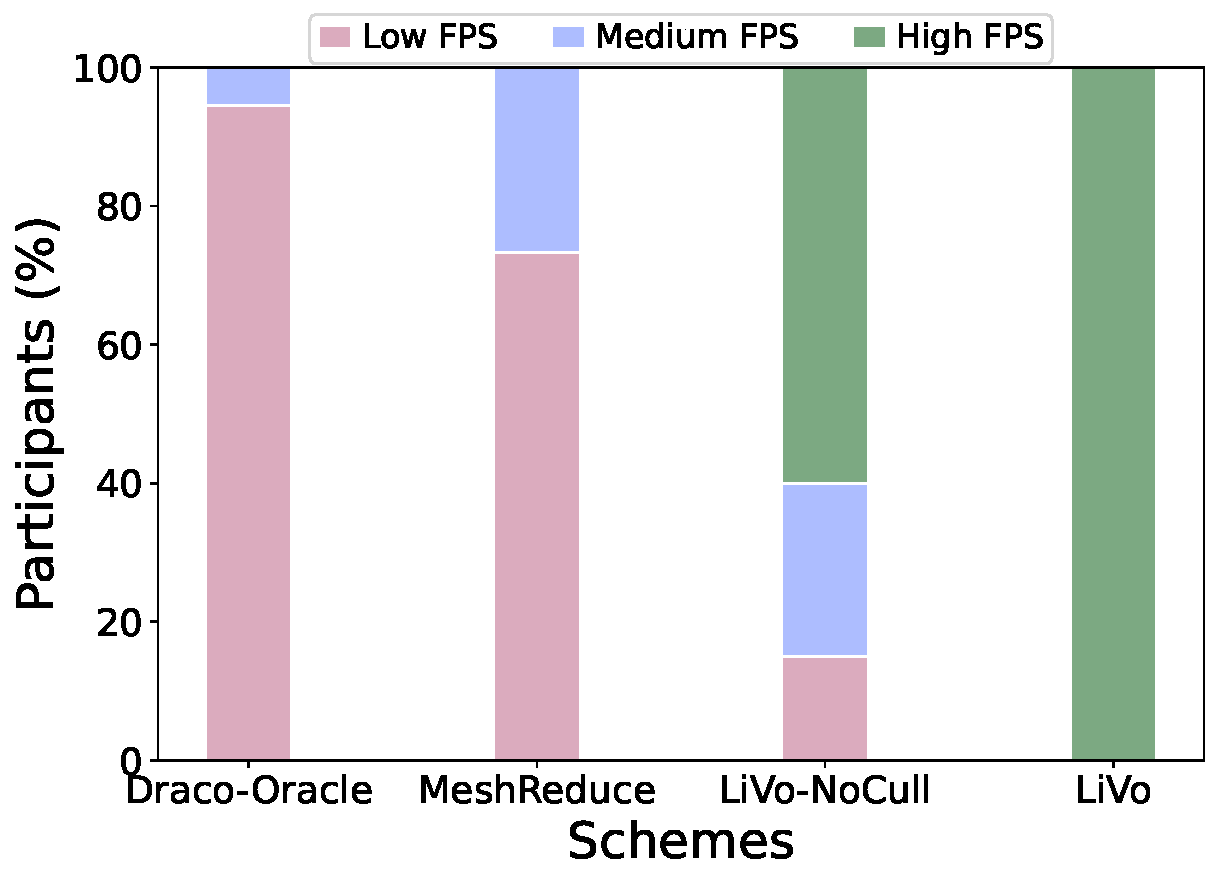
\includegraphics[width=\columnwidth]{figures/user_study_fps_distribution.pdf}
%     \caption{Feedback on fps.}
%     \label{plot:user_study_fps}
%      \end{subfigure}
%         \caption{Summary of user feedback.}
%         \label{plot:user_study_summary}
% \end{figure}

\subsection{Depth vs Color Distortion}
\cref{plot:bitrate-distortion} studies variability in PSSIM quality metric in depth (sim. color) when we fix color (sim. depth) bitrate and vary depth bitrate. \cref{plot:depth-distortion} shows how PSSIM Geometry metric varies when we increase depth bitrate (normalized as depth bitrate per point); similarly report PSSIM color in \cref{plot:color-distortion}. We observe that depth varies a lot with increase in bitrate before it flattens, while variation in color quality is minimal. Also, the bitrate that needs be allocated for depth is almost $7\times$ higher before it saturates (around vertical dotted line). This confirms that depth is much more sensitive to color and needs careful bitrate allocation.
%
\begin{figure}[t]
    \centering
    \begin{subfigure}[b]{0.49\columnwidth}
         \centering
         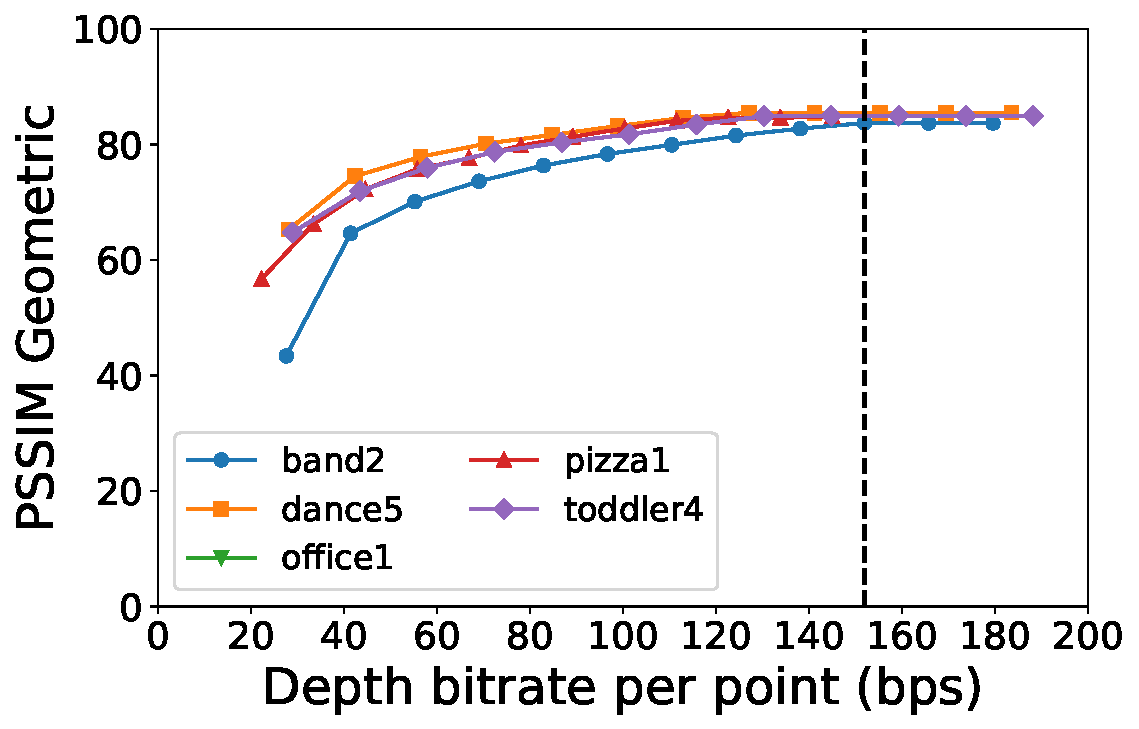
\includegraphics[width=\columnwidth]{figures/pssim_geometric_depth_per_point.pdf}
        \caption{Depth distortion vs depth bitrate.}
        \label{plot:depth-distortion}
    \end{subfigure}
    \hfill
    \begin{subfigure}[b]{0.49\columnwidth}
         \centering
         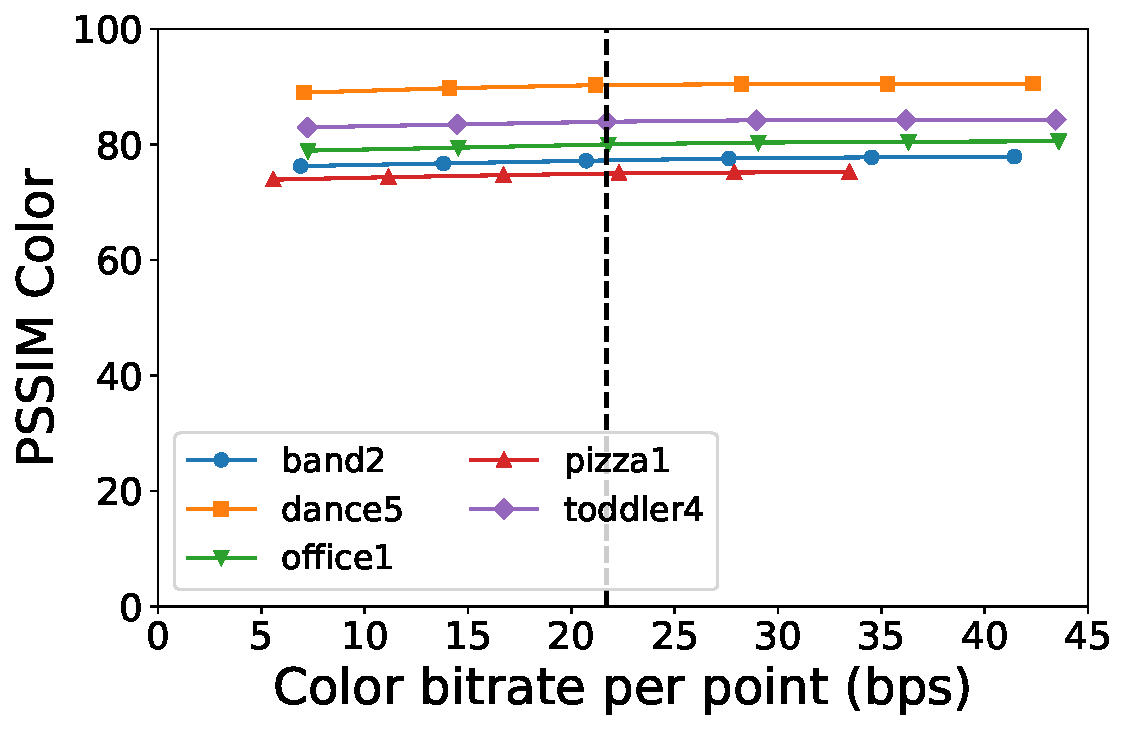
\includegraphics[width=\columnwidth]{figures/pssim_color_color_per_point.pdf}
        \caption{Color distortion vs color bitrate.}
        \label{plot:color-distortion}
    \end{subfigure}
    \caption{PSSIM distortion across videos when bitrate is varied}
    \label{plot:bitrate-distortion}
\end{figure}

\subsection{Variability in Bandwidth Traces}
\label{ss:trace_variability}

We show the variability in the 2 traces we pick - \textit{trace-1} and \textit{trace-2} in \cref{plot:mahimahi_traces}.
\begin{figure}[ht!]
  \centering 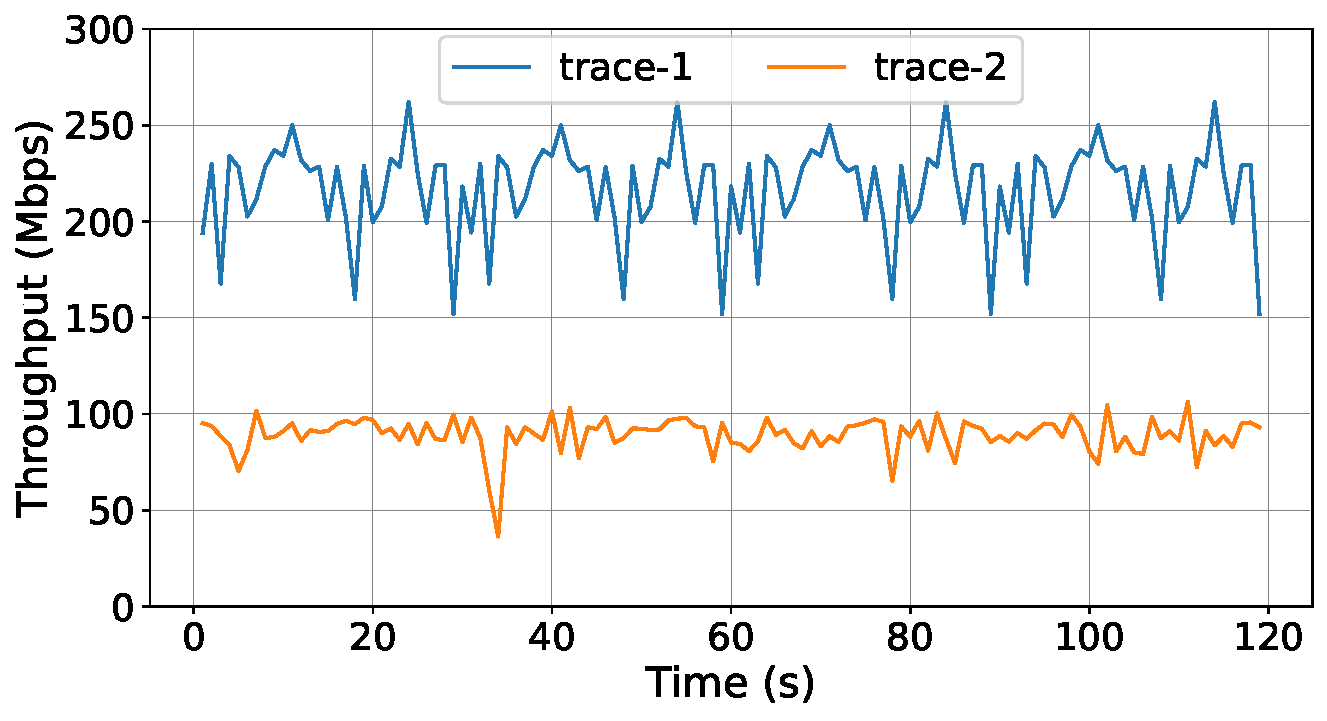
\includegraphics[width=0.8\columnwidth]{figures/throughput_wifi25_tracep1.pdf}
  \caption{Variability in the 2 network traces we consider.}
  \label{plot:mahimahi_traces}
\end{figure}

%
%
% \begin{figure*}[h!]
%   \begin{minipage}[t]{0.33\textwidth}
%     \centering
%     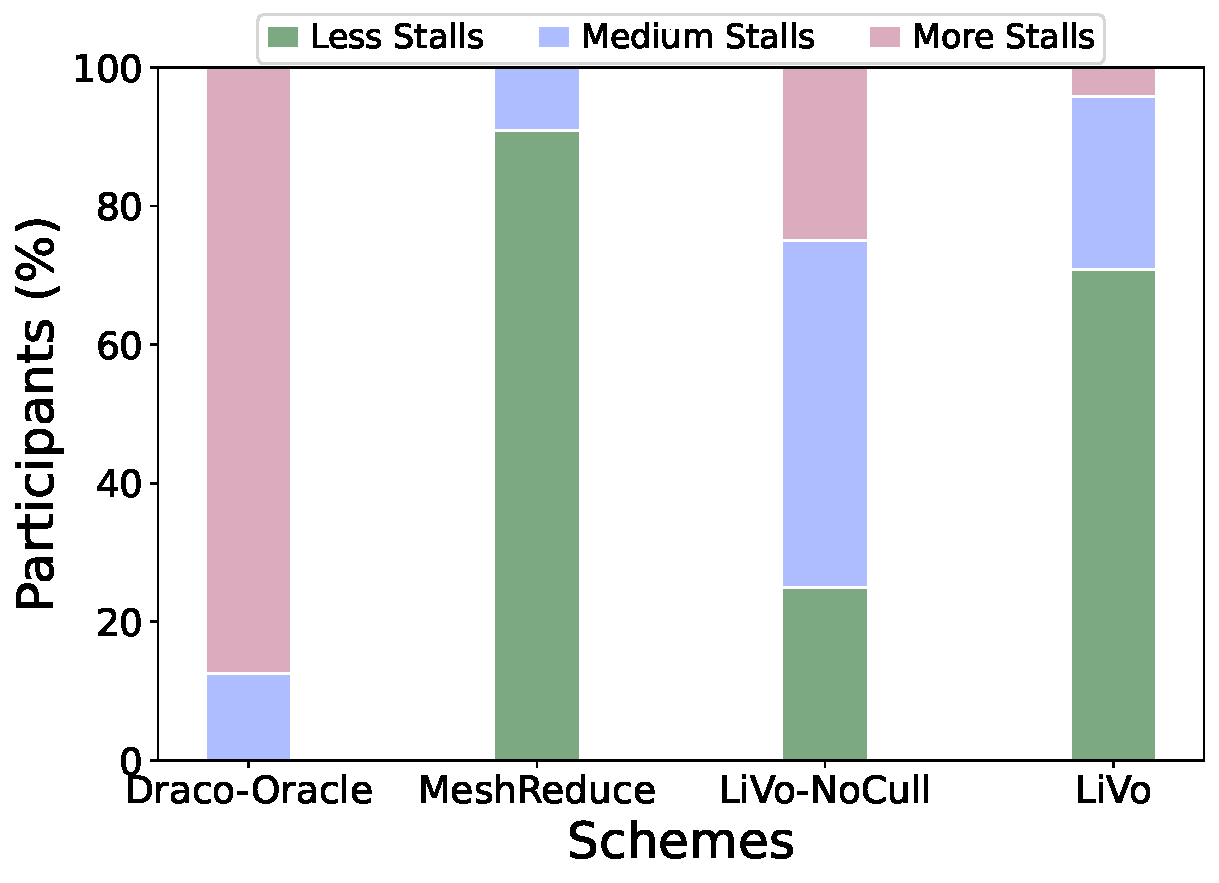
\includegraphics[width=\columnwidth]{figures/user_study_stall_distribution.pdf}
%     \caption{Feedback on stalls}
%     \label{plot:user_study_stalls}
%   \end{minipage}
%   \begin{minipage}[t]{0.33\textwidth}
%     \centering
%     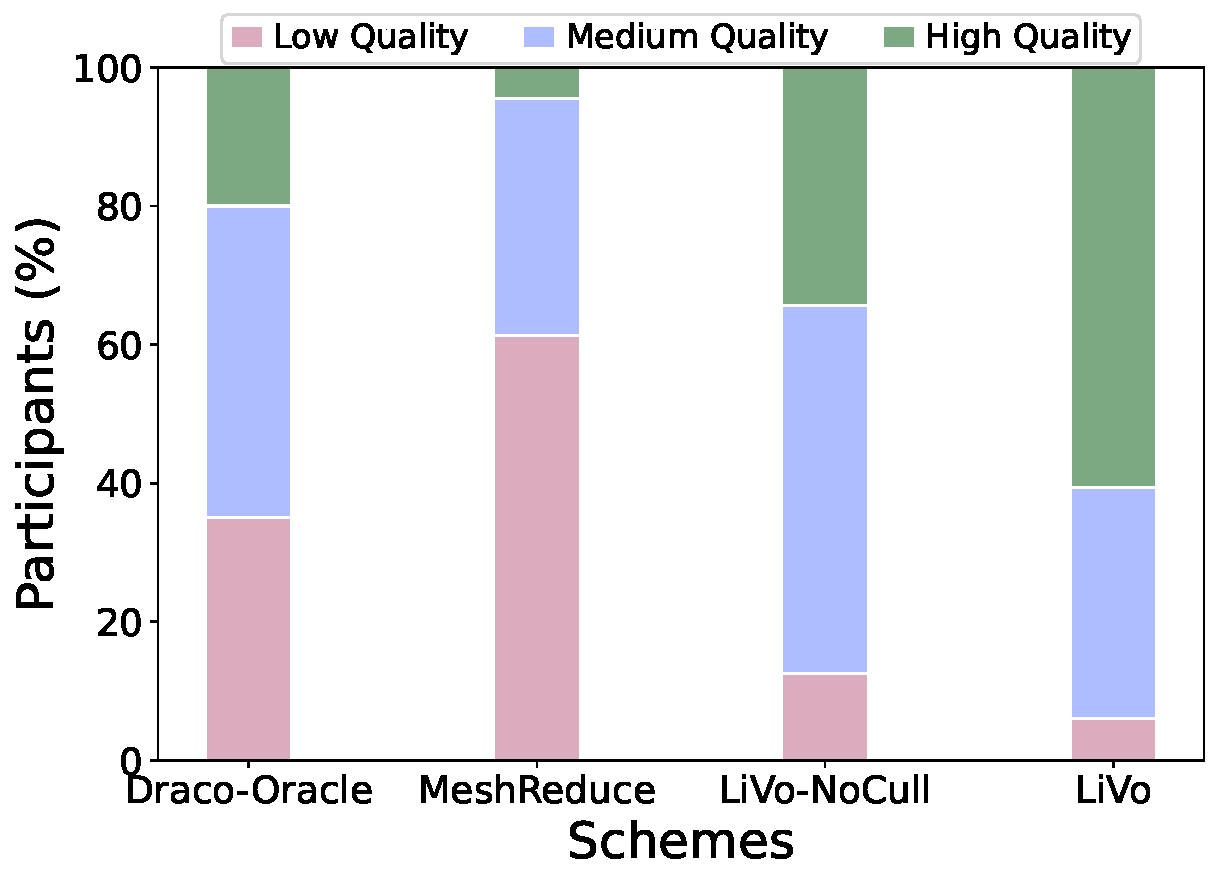
\includegraphics[width=\columnwidth]{figures/user_study_quality_distribution.pdf}
%     \caption{Feedback on quality.}
%     \label{plot:user_study_quality}
%   \end{minipage}
%   \begin{minipage}[t]{0.33\textwidth}
%     \centering 
%     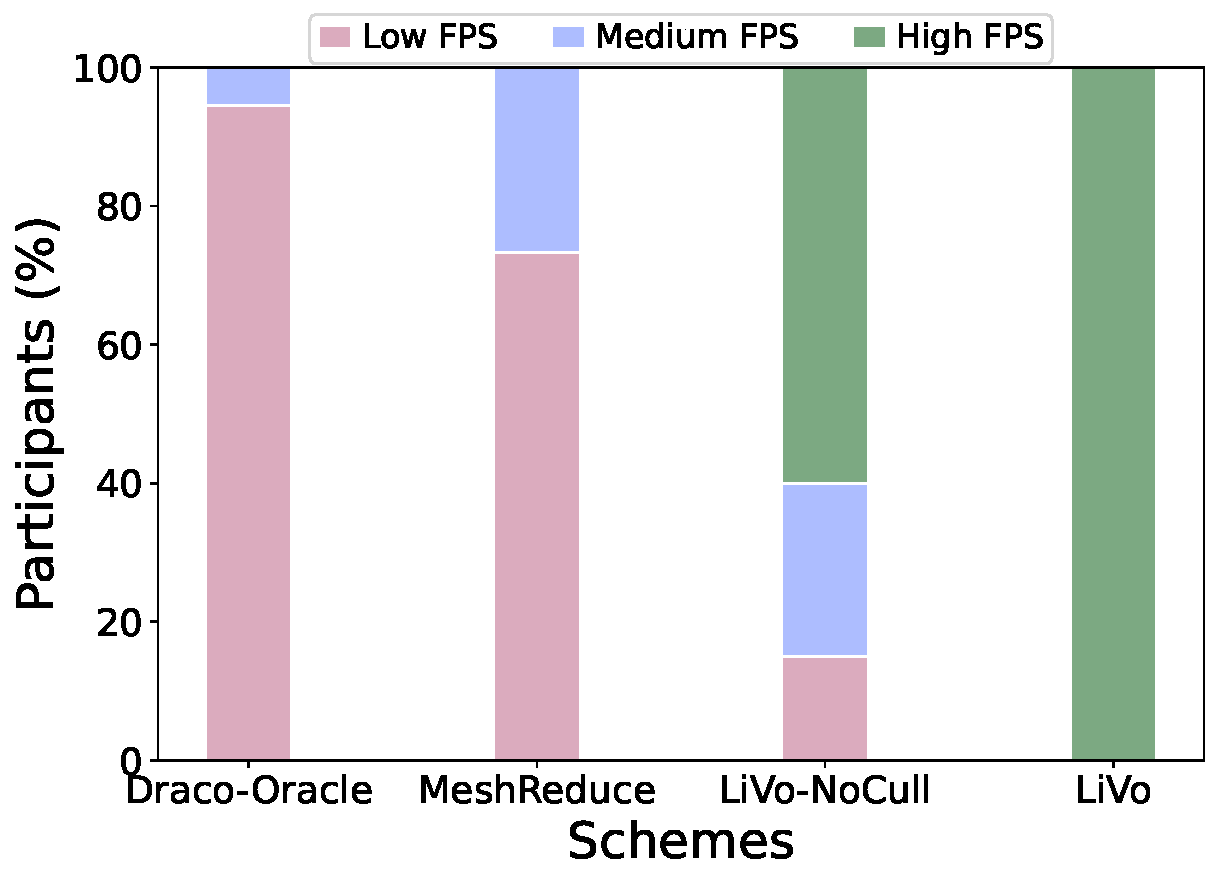
\includegraphics[width=\columnwidth]{figures/user_study_fps_distribution.pdf}
%     \caption{Feedback on FPS.}
%     \label{plot:user_study_fps}
%   \end{minipage}
% \end{figure*}
%
%

%% \begin{comment}
%% \parab{Outline.}
%% For each of the following, include a plot. The text should be a para that first describes what is being plotted, then highlights the key takeaways, and explains why the results are surprising or not.

%% \begin{itemize}
%% \item Depth encoding choice: Realsense vs our approach
%% \item Justification of Kalman filter buffer size
%% \item Justification of bandwidth split: for multiple videos, show that saturation point happens at roughly same depth per pixel.
%% \item Justify bandwidth adaptation: LiVo without bandwidth adaptation (should we do this with culling?)
%% \end{itemize}
%% \end{comment}

%% \parab{Depth Encoding.}
%% %
%% \livo encodes in Y-channel (luminance) of 3 channel 16-bit variant of H.265 encoding (Y444\_LE).
%% %
%% It also scales the depth values.
%% %
%% We also experimented with a strategy proposed by prior work~\cite{realsense-doc,depth-kautz,vrcomm} which colorizes each 16-bit depth pixel into a 3-channel RGB pixel using a depth to color conversion table.
%% %
%% \cref{plot:compression-choice} shows that \livo{}'s scaled depth encoding achieves the highest geometry and color PSSIM relative to this approach and to unscaled depth encoding.

%% %% is significantly better than encoding depth in RGB, and that depth scaling is necessary to improve quality.
%% % %
%% % When we implement this strategy inside \livo and apply to \textit{dance5} video, the average PointSSIM quality drops below 20 for both color and depth, which indicates severe quality degradation.
%% % %
%% % In contrast, naive strategy of putting depth in Y-channel (luminance) of 3 channel 16-bit variant of H.265 encoding (Y444\_LE Unscaled), improves PointSSIM geometry to above $70$.
%% % %
%% % Through visual inspection, we observed that the decoded point cloud have local block-like artifacts, which indicates that the neighbouring points have collapsed in one of the 3D dimensions (example in Appendix \cref{s:appendix}).
%% % %
%% % Our depth encoding strategy using depth scaling improves both PointSSIM color and geometry to reach 90.

%% \begin{figure}[tbp]
%%   \centering 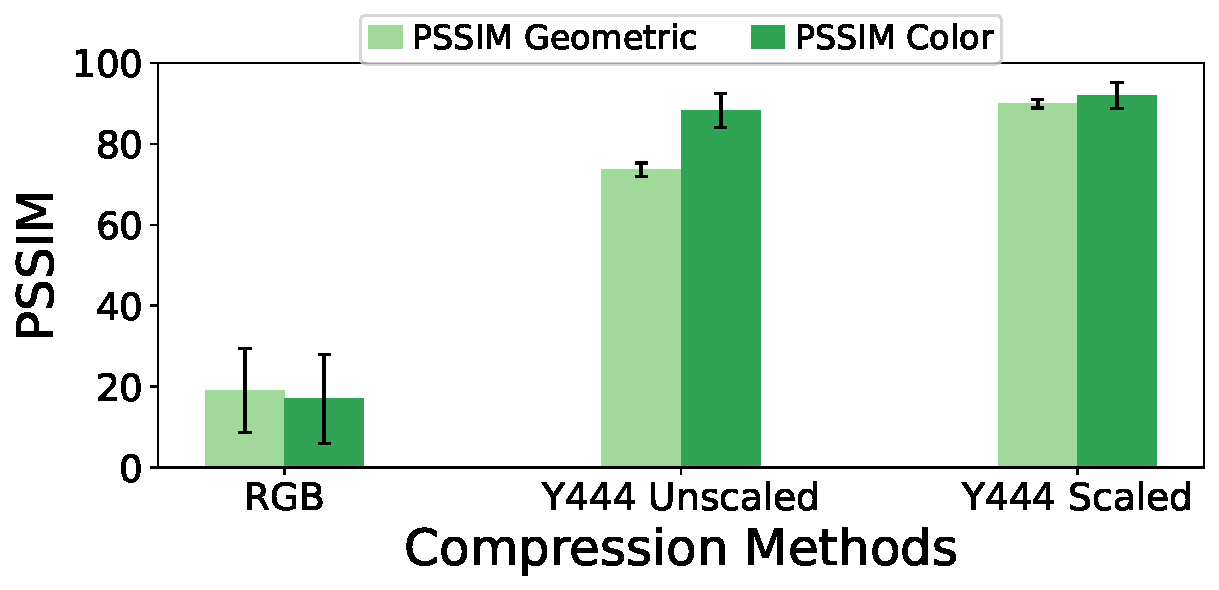
\includegraphics[width=0.5\columnwidth]{figures/pssim_compression_comparison.pdf}
%%   \caption{Comparison between realsense vs our approach.}
%%   \label{plot:compression-choice}
%% \end{figure}

%% %\harsha{Suggest moving the para below and associated table to appendix.}
%% \parab{Kalman Filter buffer size.}
%% %
%% Kalman filter prediction error depends on the prediction horizon.
%% %
%% \livo targets prediction horizons of about 10 frames (300~ms).
%% %
%% Predictions help culling, which can reduce data volume, but erroneous predictions can impact quality.
%% %
%% \livo uses a static guard-band $\epsilon$ of 20~cm around the frustum to minimize quality loss due to prediction errors.
%% %
%% \cref{tab:prediction_acc} shows that for guard-bands up to 30~cm, \livo's accuracy and data volume are relatively insensitive to the choice of guard-band, hence a static guard-band works well.
%% %
%% We have verified this for other videos as well.

%% % Prediction window is the number of lookahead frames between the last received frustum from receiver and the frustum required (through prediction) for the current outgoing frame on the sender.
%% % %
%% % We predict the frustum by running the Kalman Predictor same number of times as the prediction window size.
%% % %
%% % To correct for prediction errors, we use a guard band $\epsilon$ around the predicted frustum.
%% % %
%% % \cref{tab:prediction_acc} shows that for any prediction window size, the prediction accuracy increases with increase in the guard band size, but it comes at a cost.
%% % %
%% % Increased size of guard band results in large fraction of points in the full point cloud to fall inside the frustum; refer~\cref{tab:prediction_fraction}.
%% % %
%% % This increases unnecessary transmission of data at reduced quality.
%% % %
%% % We observe that \livo achieves an end-to-end latency <300~ms, which corresponds to a prediction window size of 10 frames (at 30~FPS).
%% % %
%% % From \cref{tab:prediction_acc}, we observe that increasing guard band size above 20~cm have marginal improvements in prediction accuracy, while saving $40\%$ of the points from transmission.
%% % %
%% % Thus, we choose $\epsilon$ to be 20~cm in \livo.

%% \begin{table}[t]
%% \centering
%%   \footnotesize
%%   \scalebox{0.8}{
%%     \begin{tabular}{|l|l|l|l|l|}
%%     \hline
%%     \multicolumn{1}{|l|}{\multirow{2}{*}{\textbf{\begin{tabular}[c]{@{}l@{}}Guard \\ Band\end{tabular}}}} & \multicolumn{4}{c|}{\textbf{Prediction Window Size}} \\ \cline{2-5} 
%%     \multicolumn{1}{|l|}{} & \multicolumn{1}{l|}{\textbf{W=5}} & \multicolumn{1}{l|}{\textbf{W=10}} & \multicolumn{1}{l|}{\textbf{W=20}} & \multicolumn{1}{l|}{\textbf{W=30}} \\ \hline
%%     10 & 98.44 (0.57) & 96.69 (0.54) & 94.37 (0.57) & 91.76 (0.57) \\ \hline
%%     20 & 99.26 (0.62) & 98.37 (0.62) & 96.13 (0.62) & 93.95 (0.62) \\ \hline
%%     30 & 99.61 (0.66) & 98.97 (0.66) & 97.22 (0.67) & 95.41 (0.67) \\ \hline
%%     50 & 99.89 (0.73) & 99.56 (0.73) & 98.46 (0.73) & 97.18 (0.73) \\ \hline
%%     \end{tabular}
%%     }
%%     \caption{Accuracy  of culling using Kalman Filter by varying the guard band (in cm) for \textit{band2}. The numbers in brackets represent fraction of points within frustum.}
%%     \label{tab:prediction_acc}
%% \end{table}

%% % \begin{table}[t]
%% % \centering
%% %   \footnotesize
%% %     \begin{tabular}{|l|l|l|l|l|}
%% %     \hline
%% %     \multicolumn{1}{|l|}{\multirow{2}{*}{\textbf{\begin{tabular}[c]{@{}l@{}}Guard Band\\ (in cm)\end{tabular}}}} & \multicolumn{4}{c|}{\textbf{Prediction Window Size}} \\ \cline{2-5} 
%% %     \multicolumn{1}{|l|}{} & \multicolumn{1}{l|}{W=5} & \multicolumn{1}{l|}{W=10} & \multicolumn{1}{l|}{W=20} & \multicolumn{1}{l|}{W=30} \\ \hline
%% %     10 & 0.57 & 0.54 & 0.57 & 0.57 \\ \hline
%% %     20 & 0.62 & 0.62 & 0.62 & 0.62 \\ \hline
%% %     30 & 0.66 & 0.66 & 0.67 & 0.67 \\ \hline
%% %     50 & 0.73 & 0.73 & 0.73 & 0.73 \\ \hline
%% %     \end{tabular}
%% %     \caption{Fraction of points within the frustum by varying guard band size for `band2' video.}
%% %     \label{tab:prediction_fraction}
%% % \end{table}

%% %
%% % \begin{figure}[t]
%% %     \centering
%% %     \begin{subfigure}[b]{0.49\columnwidth}
%% %          \centering
%% %          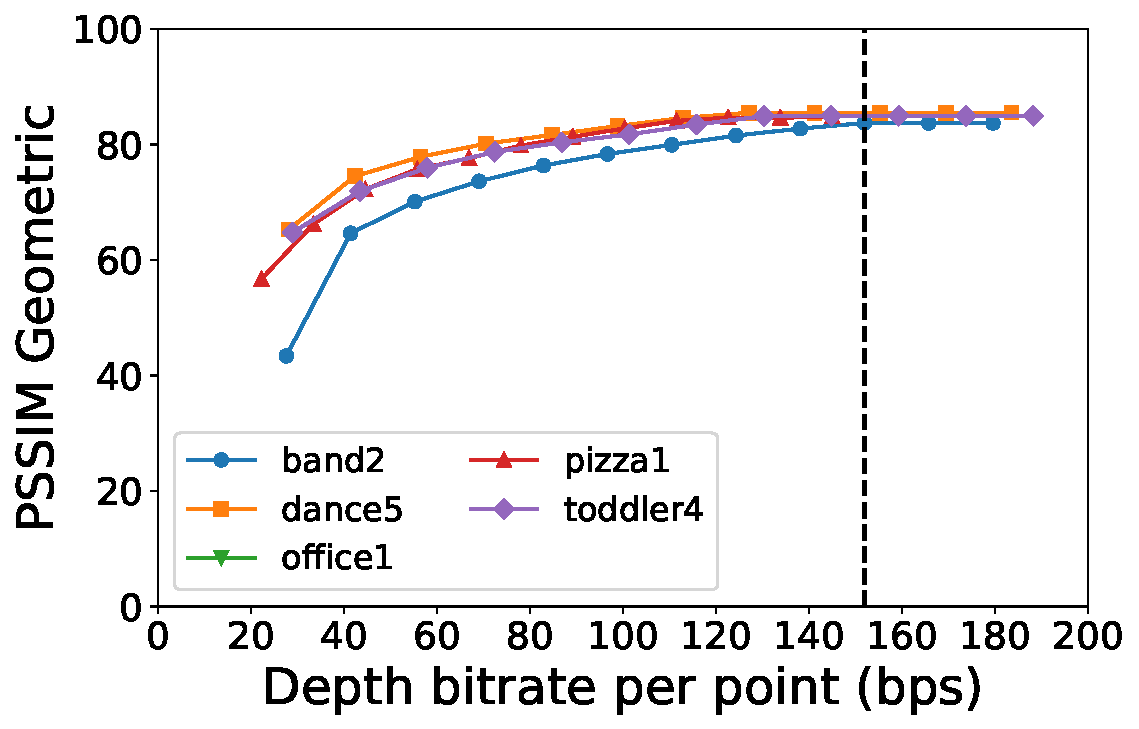
\includegraphics[width=\columnwidth]{figures/pssim_geometric_depth_per_point.pdf}
%% %         \caption{Depth distortion vs depth bitrate.}
%% %         \label{plot:depth-distortion}
%% %     \end{subfigure}
%% %     \hfill
%% %     \begin{subfigure}[b]{0.49\columnwidth}
%% %          \centering
%% %          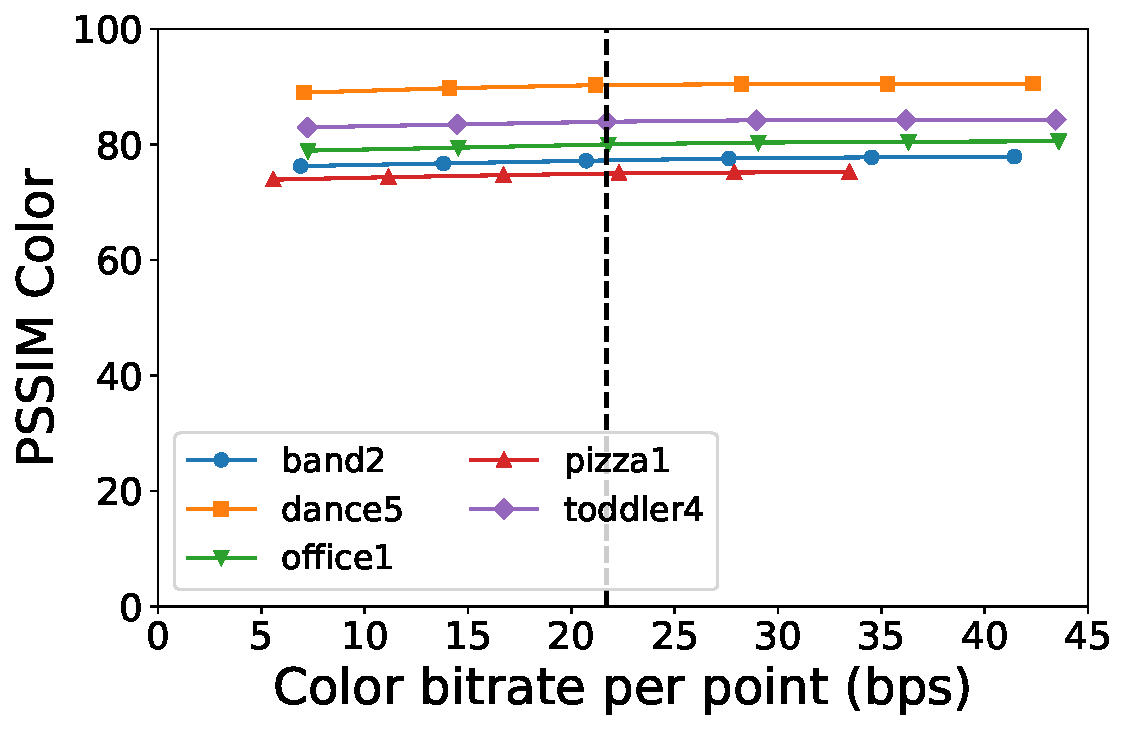
\includegraphics[width=\columnwidth]{figures/pssim_color_color_per_point.pdf}
%% %         \caption{Color distortion vs color bitrate.}
%% %         \label{plot:color-distortion}
%% %     \end{subfigure}
%% %     \caption{PSSIM distortion across videos when bitrate is varied}
%% %     \label{plot:bitrate-distortion}
%% % \end{figure}
%% %
%% %\begin{figure}[t]
%% %  \begin{minipage}[t]{0.49\columnwidth}
%% %    \centering
%% %     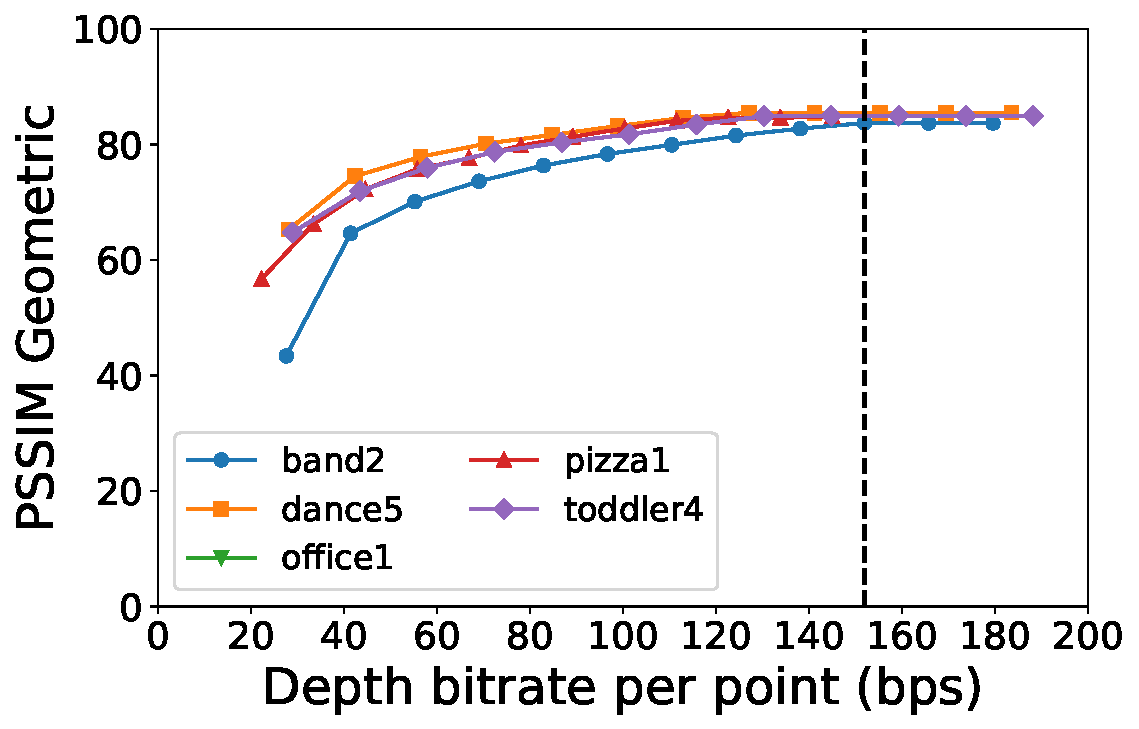
\includegraphics[width=\columnwidth]{figures/pssim_geometric_depth_per_point.pdf}
%% %    \caption{Depth distortion. \note{[Remove]}}
%% %    \label{plot:depth-distortion}
%% %  \end{minipage}
%% %  \begin{minipage}[t]{0.49\columnwidth}
%% %    \centering
%% %     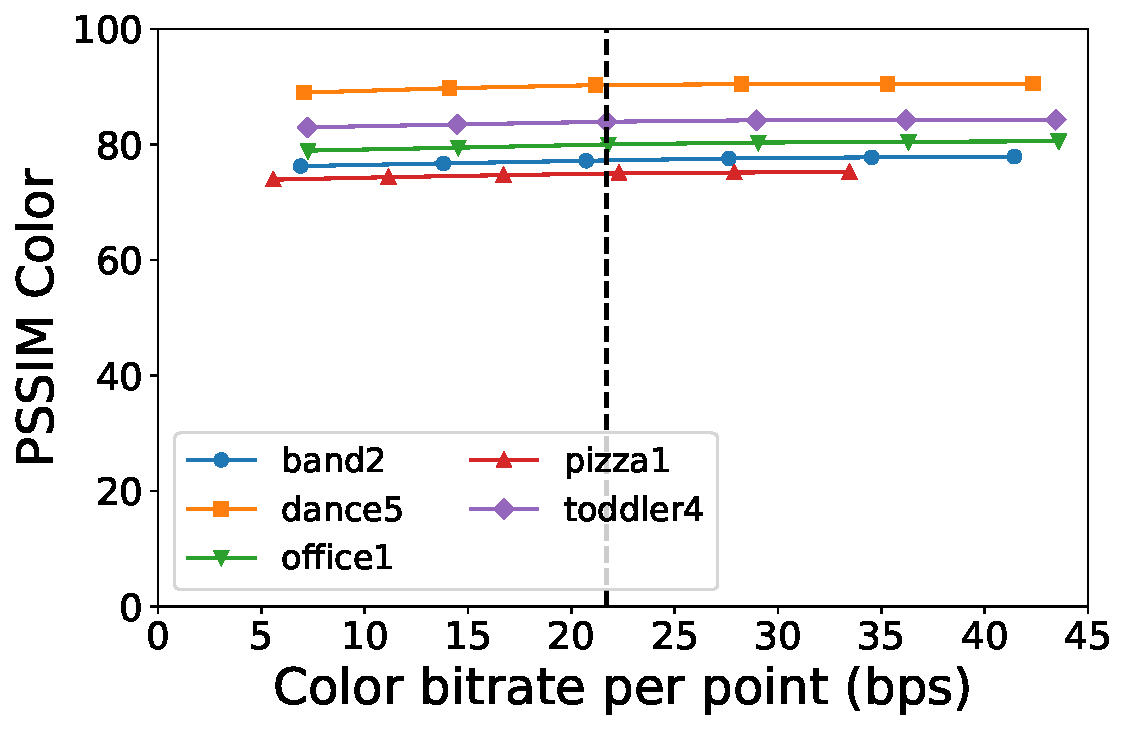
\includegraphics[width=\columnwidth]{figures/pssim_color_color_per_point.pdf}
%% %    \caption{Color distortion. \note{[Remove]}}
%% %    \label{plot:color-distortion}
%% %  \end{minipage}
%% %\end{figure}

%% \begin{figure}[t]
%%   \begin{minipage}[t]{0.49\columnwidth}
%% 	    \centering
%% 	     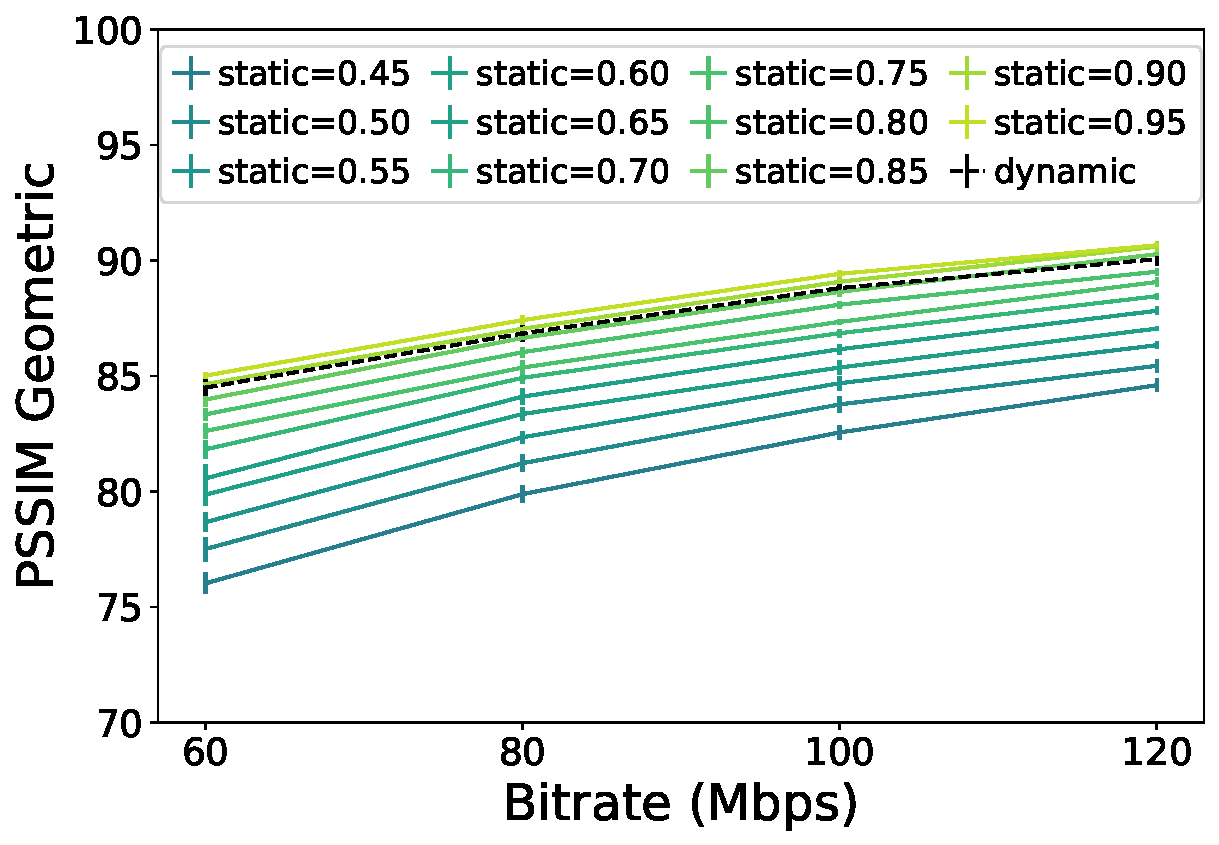
\includegraphics[width=\columnwidth]{figures/static_vs_dynamic_pssim_geo.pdf}
%% 	    \caption{PSSIM Geometric for static vs dynamic split.}
%% 	    \label{plot:split-sweep-geo}
%% 	  \end{minipage}
%%   \begin{minipage}[t]{0.49\columnwidth}
%% 	    \centering
%% 	     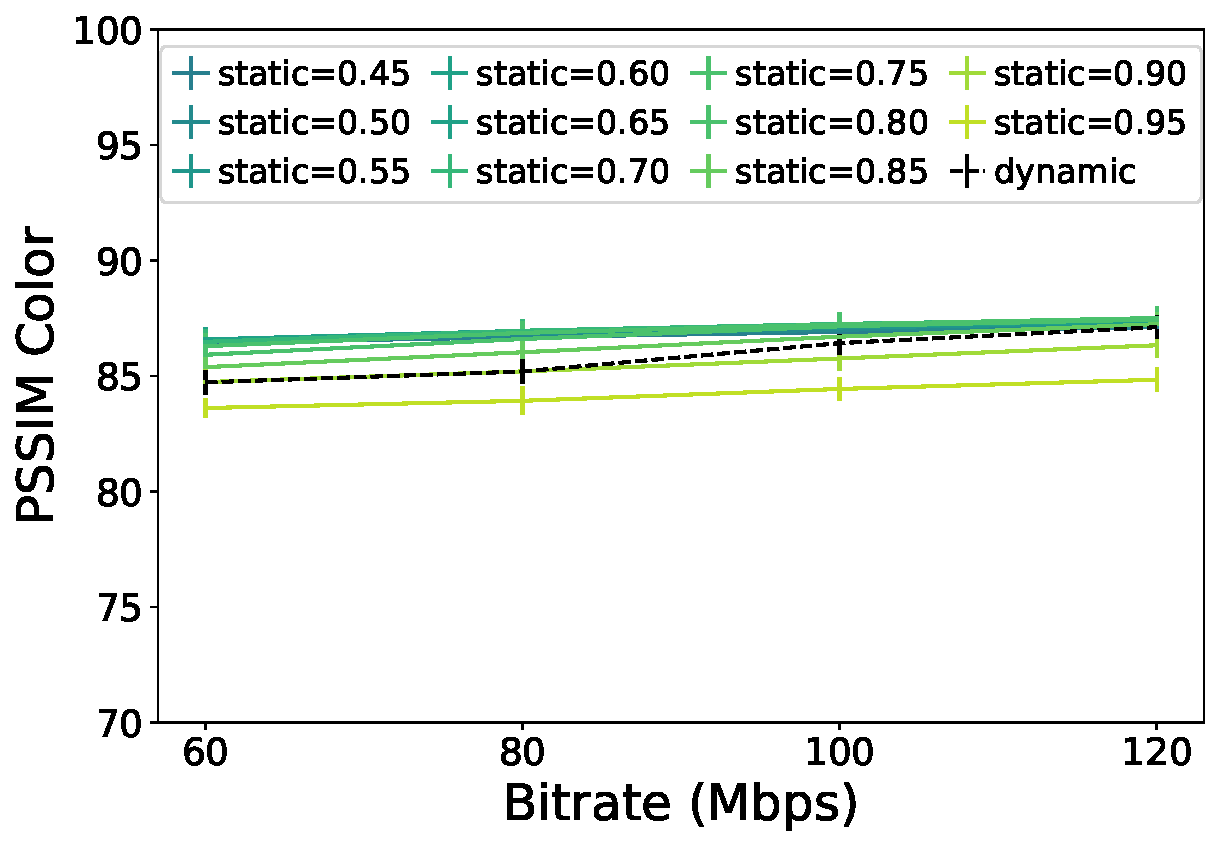
\includegraphics[width=\columnwidth]{figures/static_vs_dynamic_pssim_color.pdf}
%% 	    \caption{PSSIM Color for static vs dynamic split.}
%% 	    \label{plot:split-sweep-color}
%% 	  \end{minipage}
%% \end{figure}

%% %% \begin{figure}[t]
%% %% 	\centering 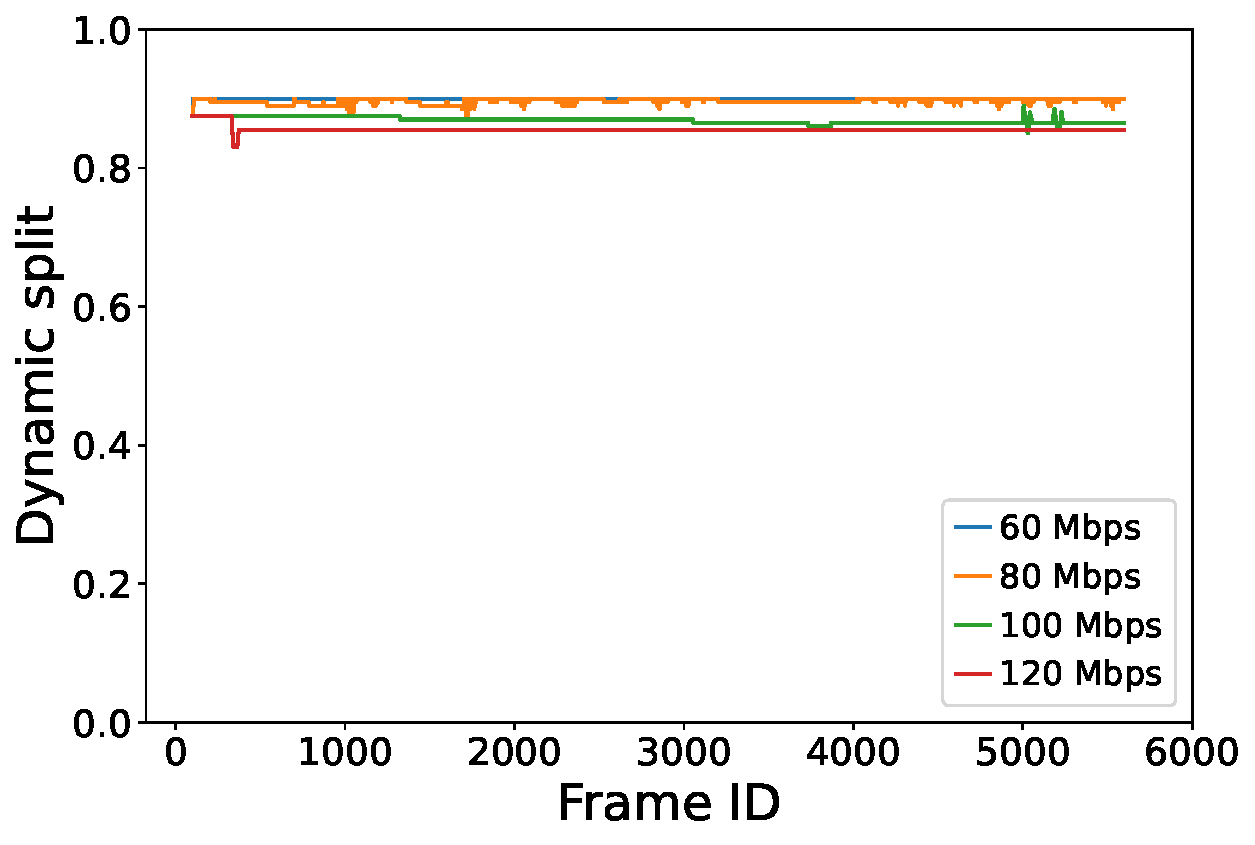
\includegraphics[width=0.5\columnwidth]{figures/split_convergence.pdf}
%% %% 	\caption{Split convergence.}
%% %% 	\label{plot:split-convergence}
%% %% \end{figure}

%% \parab{Bandwidth Splitting.}
%% %
%% %\cref{plot:depth-distortion} plots depth PSSIM as a function of bits per second per point, when color is assigned a high (100~Mbps) rate.
%% %
%% %Across all our videos, depth quality saturates at about 152 bits per second per point.
%% %
%% %Conversely, when depth bit rate is fixed, color PSSIM saturates at about 22 bits per second (\cref{plot:color-distortion}).
%% %
%% %Perceptual quality in 3D is more sensitive to depth encoding than color, since loss in depth leads to geometrical errors that can distort a 3D representation of an object.
%% %
%% %This justifies our choice of 7:1 as the ratio of depth to color per point.
%% %
%% \cref{plot:split-sweep-geo} plots compares PSSIM for different static splits with \livo{}'s dynamic split (\cref{ss:bw-adaptation}) for bitrates ranging from 60-120~Mbps for \textit{office1} (similarly, color in \cref{plot:split-sweep-color}).
%% %
%% Dynamic splitting is with 0.5 PSSIM points for geometry and 3 PSSIM points for color relative to the best static split.
%% %
%% As available bandwidth increases, both geometry and color PSSIM values are within 0.5 of the best static split.
%% %
%% This demonstrates the effectiveness of dynamic splitting.
%% %
%% %% \cref{plot:split-convergence} shows how quickly the bitrate split converges when the scene complexity changes. 
%% %
%% Moreover, dynamic splitting converges quickly, within 5-10 frames (figure omitted for brevity).
%% %
%% %Also, the split variation occurs more for bandwidth limited than bandwidth adequate regions.
%% %

%% \parab{Bandwidth Adaptation.}
%% %
%% % \begin{figure}[t]
%% %      \centering
%% %      \begin{subfigure}[b]{0.49\columnwidth}
%% %          \centering
%% %          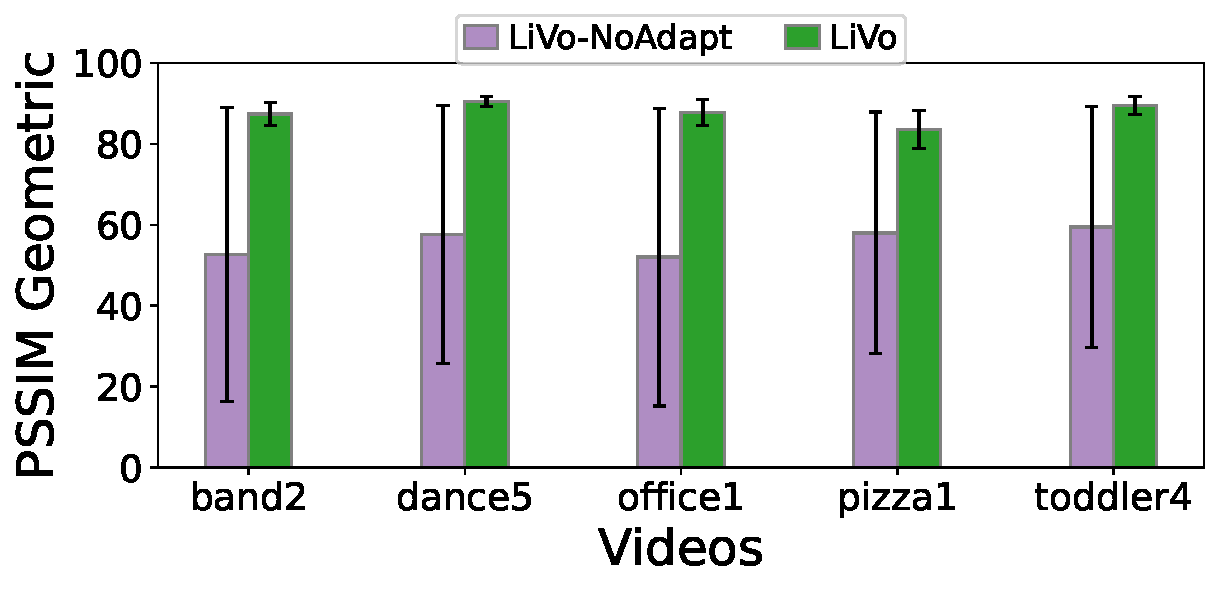
\includegraphics[width=\columnwidth]{figures/pssim_geo_starline_livo.pdf}
%% %          \caption{Geometry}
%% %          \label{plot:pssim_geo_starline_livo}
%% %      \end{subfigure}
%% %      \hfill
%% %      \begin{subfigure}[b]{0.49\columnwidth}
%% %          \centering
%% %          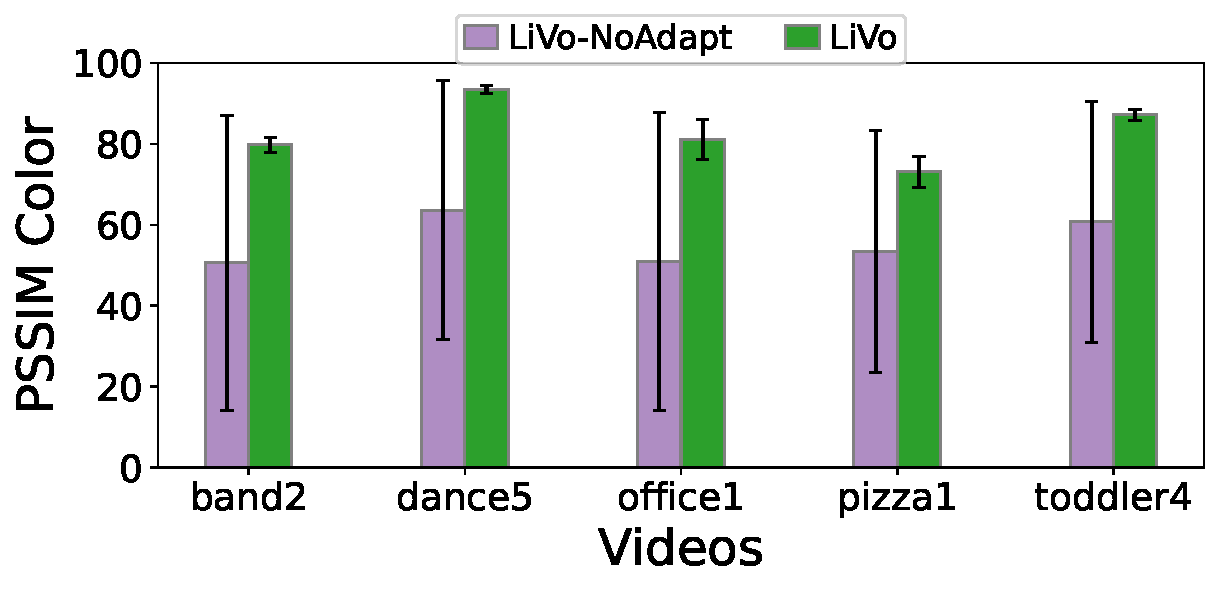
\includegraphics[width=\columnwidth]{figures/pssim_color_starline_livo.pdf}
%% %          \caption{Color}
%% %          \label{plot:pssim_color_starline_livo}
%% %      \end{subfigure}
%% %     \caption{PSSIM metric for Starline (no adaptation) vs \livo}
%% %     \label{plot:pssim_starline_livo}
%% % \end{figure}
%% %
%% \begin{figure}[t]
%%   \begin{minipage}[t]{0.49\columnwidth}
%%     \centering
%%      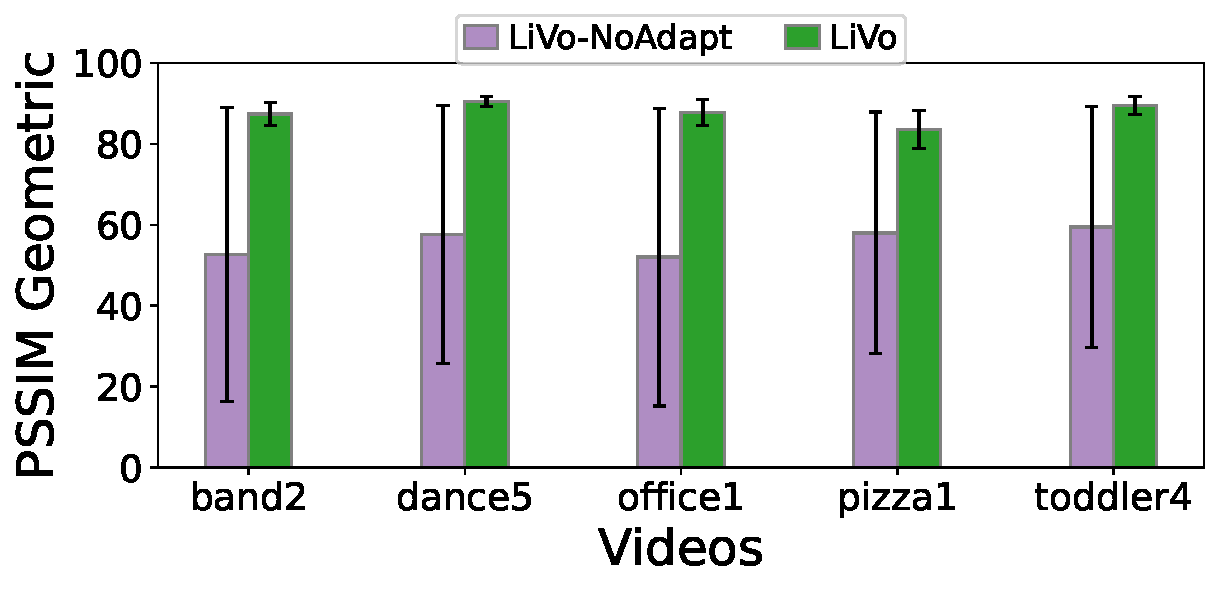
\includegraphics[width=\columnwidth]{figures/pssim_geo_starline_livo.pdf}
%%     \caption{PSSIM Geometric, \livo-NoAdapt vs \livo.}
%%     \label{plot:pssim_geo_starline_livo}
%%   \end{minipage}
%%   \begin{minipage}[t]{0.49\columnwidth}
%%     \centering
%%      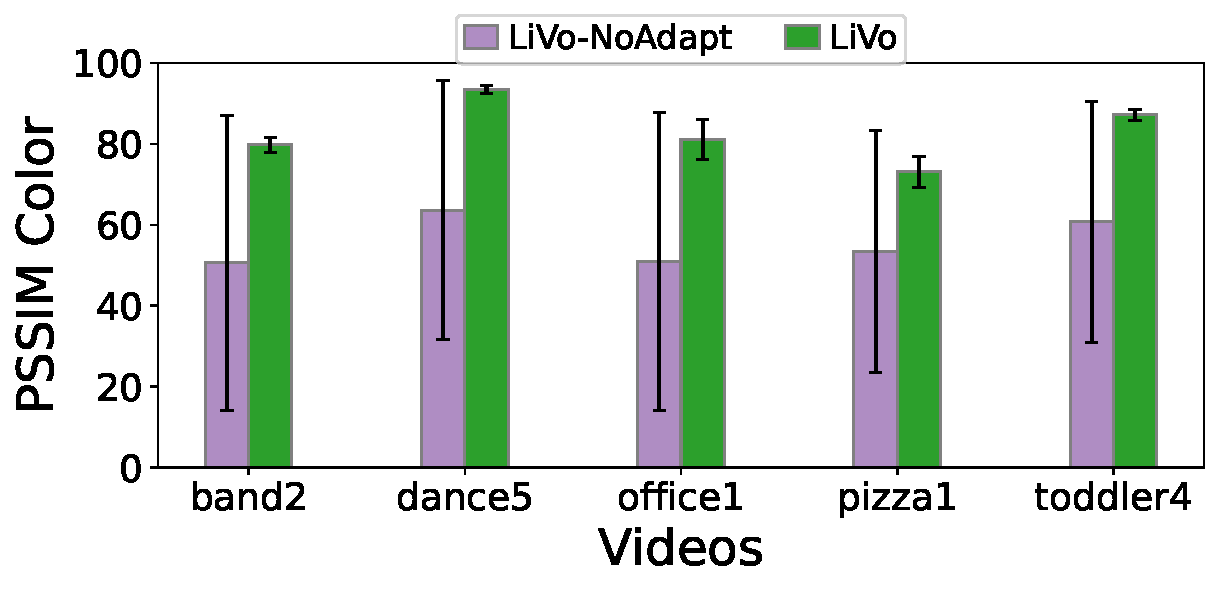
\includegraphics[width=\columnwidth]{figures/pssim_color_starline_livo.pdf}
%%     \caption{PSSIM Color, \livo-NoAdapt vs \livo.}
%%     \label{plot:pssim_color_starline_livo}
%%   \end{minipage}
%% \end{figure}
%% %
%% What if LiVo did not use bandwidth-adaptation and view culling at all, but instead used fixed quality parameters?
%% %
%% We set fixed color QP (quantization parameter) to 22 and depth QP to 14; Starline~\cite{starline} uses these values.
%% %
%% \cref{plot:pssim_geo_starline_livo} and \cref{plot:pssim_color_starline_livo} show that this LiVo-NoAdapt has significant quality drop of $30-41\%$ for geometry and $27-37\%$ for color, with PSSIM going below 60.

%% \parab{Frustum Prediction.}
%% %
%% \begin{table}[t]
%% \centering
%% \footnotesize
%%     \scalebox{0.8}
%%     {
%% 	\begin{tabular}{|l|l|l|l|}
%% 		\hline
%% 		\textbf{Method} & \textbf{\begin{tabular}[c]{@{}l@{}}\# Hidden \\ Units\end{tabular}} & \textbf{\begin{tabular}[c]{@{}l@{}}Position \\ (m)\end{tabular}} & \textbf{\begin{tabular}[c]{@{}l@{}}Rotation \\ (degree)\end{tabular}} \\ \hline
%% 		\multirow{3}{*}{\begin{tabular}[c]{@{}l@{}}MLP\\ Trained on \\ 1 user trace\end{tabular}} & 3 & 1.01 & 135.86 \\ \cline{2-4} 
%% 		& 32 & 0.59 & 80.46 \\ \cline{2-4} 
%% 		& 64 & 0.24 & 58.24 \\ \hline
%% 		\multirow{3}{*}{\begin{tabular}[c]{@{}l@{}}MLP\\ Trained on\\ 2 user trace\end{tabular}} & 3 & 0.40 & 33.34 \\ \cline{2-4} 
%% 		& 32 & 0.09 & 3.69 \\ \cline{2-4} 
%% 		& 64 & 0.07 & 2.17 \\ \hline
%% 		Kalman Filter & - & 0.04 & 7.19 \\ \hline
%% 	\end{tabular}
%%     }
%% 	\caption{Comparing prediction errors in Kalman Filter-based to learning-based prediction methods.} % For band2 video
%% 	\label{tab:frustum_kf_learning}
%% \end{table}
%% %
%% To estimate quality impairment as a result of our predictive culling, we compare it against LiVo with perfect culling (using predictions obtained from the user trace).
%% %
%% The average quality difference in PSSIM geometry and color is $1\%$ across all 5 videos when run on \textit{trace-1}.

%% Prior work has trained frustum predictors from user traces~\cite{vues,vivo} for on-demand volumetric videos.
%% %
%% This doesn't quite apply to conferencing, since user interactions depend on content, which can be different for different content.
%% %
%% That said, we evaluate (\cref{tab:frustum_kf_learning}) whether an MPL with 3 hidden layers used in ViVo~\cite{vivo} could learn from a small number of our traces.
%% %
%% We find that it may be possible to match LiVo's predictor only with a large number of hidden layers (64); with the three that ViVo uses, prediction errors are unacceptably high.

%% %% Learning method-based frustum predictions have been proposed in on-demand streaming~\cite{vivo,vues}.
%% %% %
%% %% Though these methods aren't suitable for conferencing~\cref{ss:view-prediction-and-culling}, we consider a scenario where user traces for same conferencing setup is available.
%% %% %
%% %% We train an multi-layer perceptron (MLP) with 1 hidden layer used in ViVo's~\cite{vivo} prediction on 1 and 2 user traces and tested on the rest for \textit{band2}.
%% %% %
%% %% \cref{tab:frustum_kf_learning} shows that 3 hidden units (used in ViVo) has position and rotational error of $40~cm-1~m$ and $33-135~degrees$, respectively; this model is unusable. 
%% %% %
%% %% Increasing the number of user traces and hidden units bring down the error to usable numbers.
%% %% %
%% %% \livo's Kalman Filter-based prediction consistently achieves less than $4~cm$ of positional and $7~degrees$ of rotational error.
